\documentclass[runningheads]{llncs}

\usepackage[long,nodayofweek,level,12hr]{datetime}
\usepackage{graphicx}
\usepackage{hyperref}
\usepackage{caption}
\usepackage[utf8]{inputenc}
\usepackage{multirow}
\usepackage{tikz}
\usepackage{amssymb}
\usepackage{physics}
\usepackage{stmaryrd}
\usepackage{cleveref}
\usepackage{algorithm}
\usepackage{algpseudocode}
\usepackage{varwidth}
\usepackage{cite}

\floatname{algorithm}{Sub-routine}

\makeatletter
\renewcommand\subsubsection{\@startsection{subsubsection}{3}{\z@}%
                       {-18\p@ \@plus -4\p@ \@minus -4\p@}%
                       {0.5em \@plus 0.22em \@minus 0.1em}%
                       {\normalfont\normalsize\bfseries\boldmath}}
\makeatother

\setcounter{secnumdepth}{3}
\numberwithin{equation}{section}

\title{
    CRYSTALS\\(CRYptographic SuiTe for Algebraic LatticeS):\\ A New (Classical) Post-Quantum\\Public-Key Cryptosystem Standard
}

\subtitle{    
    \vspace{4ex} Advanced Topics in Information Security /\\ Cryptography and Security Protocols\\ \vspace{2ex} \normalsize Ph.D. (Doctoral Program) in Information Security\\ \vspace{2ex} \normalsize Instituto Superior T\'{e}cnico, University of Lisbon\\(2022/2023 - 2${}^{\mathrm{nd}}$ Semester)
    \vspace{-3ex}
}

\titlerunning{
    CRYSTALS: A (Classical) Post-Quantum Public-Key Cryptosystem
}

\author{
    R\'{u}ben Barreiro\inst{1}\thanks{Student Identification: IST1108107} \and
    Paulo Mateus\inst{1,2}\thanks{Acknowledgments and thanks to Prof. Paulo Mateus, who is the lecturer of\break the course ``Advanced Topics in Information Security / Cryptography and Security\break Protocols'' at Instituto Superior T\'{e}cnico, University of Lisbon, Portugal.}
}

\authorrunning{R\'{u}ben Barreiro et al.}

\institute{
    Instituto Superior T\'{e}cnico, University of Lisbon, Portugal\\
    \email{\{ruben.andre.letra.barreiro,paulo.mateus\}\\@tecnico.ulisboa.pt} \and
    Instituto de Telecomunica\c{c}\~{o}es, Portugal\\
    \email{paulo.mateus@lx.it.pt}
}

\date{\today}


\begin{document}

    \maketitle
    
    \vspace{2ex}

    \hrule

    \vspace{-1ex}
    \begin{figure}[!h]
        \centering
        
\includegraphics[width=0.54\linewidth]{figures/logos/cryptosystem/crystals-cryptosystem.pdf}\\
        \begin{minipage}{.5\textwidth}
            \centering
            \vspace{-6ex}
            
\includegraphics[width=0.9\linewidth]{figures/logos/college-and-r&d-labs/university-of-lisbon-horizontal-logo.pdf}
        \end{minipage}%
        \hspace{-12ex}
        \begin{minipage}{.5\textwidth}
            \centering
            \vspace{-6ex}
            
\includegraphics[width=0.9\linewidth]{figures/logos/college-and-r&d-labs/instituto-superior-tecnico-horizontal-logo.pdf}
        \end{minipage}\\
        \vspace{-8ex}
        
\includegraphics[width=0.4\linewidth]{figures/logos/college-and-r&d-labs/instituto-telecomunicacoes-logo.pdf}
    \end{figure}
    \vspace{-1ex}

    \hrule
    
    \newpage

    \begin{abstract}
        In the last few years, Quantum Computing has been growing\break exponentially, and several quantum algorithms are threatening most of the cryptography we are using nowadays. In 1994, Peter Shor proposed one of them, known nowadays as Shor’s algorithm. This quantum\break algorithm is capable of factoring large integer numbers into smaller prime numbers and finding discrete logarithms in a polylogarithmic time. These two problems are considered hard to solve on a classical computer, and\break we apply this computational hardness assumption as the basis of several\break cryptosystems we used since the 1970s. For instance, the security factor\break of popular cryptosystems, such as Rivest-Shamir Adleman (RSA),\break Diffie-Hellman (DH), and Elliptic-Curve Cryptography (ECC), rely on this assumption. However, this hardness assumption does not hold for\break quantum computers due to the expected impact of Shor's algorithm.

        Concerning this imminent threat, the scientific community is putting enormous efforts into selecting new quantum-resistant candidates, arising\break two new leading families of quantum-resistant cryptography, known as (Classical) Post Quantum Cryptography and Quantum Cryptography. For the former, we consider mathematical approaches and problems\break believed to be computationally hard to solve using both classical and\break quantum computers. From this family of candidates, we have a popular set of cryptographic primitives based on mathematical problems related to algebraic lattices, commonly known as Lattice-based Cryptography.
        
        In this paper/report, we discuss Lattice-based Cryptography in detail, its fundamentals, as well as the respective mathematical and computational\break hardness assumptions involved, presenting a detailed description and analysis of CRYptographic SuiTe for Algebraic LatticeS (CRYSTALS) public-key cryptosystem, namely its variants for asymmetric encryption (CRYSTALS-Kyber) and digital signatures (CRYSTALS-Dilithium),\break already selected as the new (and first-ever) standards for public-key\break cryptography to be adopted at the beginning of the post-quantum era.
    \end{abstract}

    \section{Background}
    \label{sec:background}

    Recently, due to the emergence of Quantum Computing and its expected future impact on Modern Cryptography, from the threats arising from some quantum algorithms such as Grover's \cite{grover:fast-quantum-mechanical-algorithm-database-search:1996:06-2024}, Simon's \cite{simon:power-quantum-computation:1997:06-2024}, Brassard-Hoyer-Tapp (BHT) \cite{brassard-hoyer-tapp:quantum-cryptanalysis-hash-and-claw-free-functions:1998:06-2024}, and Shor's \cite{shor:algorithms-quantum-computation-discrete-logarithms-and-factoring:1994:06-2024,shor:polynomial-time-algorithms-prime-factorization-and-discrete-logarithms-quantum-computer:1997:06-2024} algorithms, new quantum-resistant cryptosystems are being studied.
    
    These new alternatives of Modern Cryptography are mainly focused on Key Exchanges and Public-Key Cryptography since the expected impacts of Grover's, Simon's, and BHT algorithms on Symmetric Cryptography and Cryptographic Hash Functions are minor when compared to the impact Shor's algorithm will have on Asymmetric Cryptography and Public-Key Cryptosystems we use.
    
    We support this claim since we expect symmetric encryption and\break cryptographic hash algorithms to have their security strength only reduced by half and by a third, respectively. For instance, symmetric encryption algorithms, such as Advanced Encryption Standard (AES) \cite{daemen-rijmen:block-cipher-rijndael:2000:06-2024}, are currently believed to be quantum-resistant when we use them with key sizes doubled regarding what we consider secure nowadays in order to resist to brute-force attacks made by Grover's and Simon's algorithms\footnote{For AES, 256 bits are considered quantum-resistant.}. Similarly, cryptographic hash algorithms and functions, such as Secure Hash Algorithm (SHA) \cite{dworkin:sha-3-standard-permutation-based-hash-and-extendable-output-functions:2015:06-2024}, are currently believed to be quantum-resistant when we use them with output sizes tripled regarding what we consider secure today in order to resist to collision, claw-finding, and birthday attacks made by BHT algorithm, also known as Quantum Birthday Attack \footnote{For SHA, 384 bits or more, are believed to be quantum-resistant.}.

    In the opposite direction, we expect the Asymmetric and Public-Key\break Cryptography we currently use nowadays to be easily ``broken'' by Shor's\break algorithm in polylogarithmic time, running in a sufficiently powerful Quantum\break Computer with a large processing capacity, no matter how large the keys used are nor how we change the security parameters. This claim is valid since Shor's algorithm can solve the factorization of large integer numbers into smaller prime numbers as well as the discrete logarithm problem in a very efficient fashion,\break while most of the currently used public-key cryptosystems, digital signature schemes, and key exchange protocols in our lives, such as Rivest-Shamir-Adleman (RSA) \cite{rivest-shamir-adleman:method-digital-signatures-and-public-key-cryptosystems:1978:06-2024}, Diffie-Hellman (DH) \cite{diffie-hellman:new-directions-cryptography:1976:06-2024,merkle:secure-communications-over-insecure-channels:1978:06-2024}, ElGamal \cite{elgamal:public-key-cryptosystem-signature-scheme-based-discrete-logarithms:1985:06-2024}, Digital Signature Algorithm\break (DSA) \cite{schnorr:efficient-identification-and-signatures-smart-card:1990:06-2024,schnorr:efficient-signature-generation-smart-cards:1991:06-2024,chen-moody-regenscheid-robinson:digital-signature-standard:2023:06-2024}, and other primitives based on Elliptic-Curve Cryptography (ECC) \cite{miller:use-elliptic-curves-cryptography:1986:06-2024,koblitz:elliptic-curve-cryptosystems:1987:06-2024}, have their security relied precisely on the computational hardness from these two mathematical problems when we consider only classical contexts.\break However, for quantum contexts, all these cryptographic primitives will become obsolete and that is the reason why we need to replace them in the future.

    From this incoming need, two new major families of Modern Cryptography\break arose, one named (Classical) Post-Quantum Cryptography \cite{bernstein-buchmann-dahmen:post-quantum-cryptography:2009:06-2024,bernstein-lange:post-quantum-cryptography:2017:06-2024} and the other named Quantum Cryptography \cite{wiesner:conjugate-coding:1983:06-2024,brassard-crepeau:quantum-cryptography:2005:06-2024,ekert:quantum-cryptography-based-bell-theorem:1991:06-2024,pirandola-et-al:advances-quantum-cryptography:2020:06-2024,grasselli:quantum-cryptography-key-distribution-conference-key-agreement:2021:06-2024,vidick-wehner:introduction-quantum-cryptographic:2023:06-2024}, as the more suitable candidates to\break replace the cryptographic primitives we use today, which we will start to refer to as (Classical) Pre-Quantum Cryptography to clarify the presented nomenclature.    
    
    The former is very similar to the cryptographic primitives we currently use in (Classical) Pre-Quantum Cryptography and also uses classical information (in the form of bits). However, (Classical) Post-Quantum Cryptography has its basis in mathematical problems and computational assumptions we believe to be hard to be solved by a classical computer and even by a considerably powerful\break quantum computer. In particular, we have several categories of (Classical)\break Post-Quantum Cryptography differing on what type of mathematical problems they have their computational hardness assumptions based on, such as\break Lattice-based Cryptography \cite{goldreich-goldwasser-halevi:public-key-cryptosystems-from-lattice-reduction-problems:1997:06-2024,hoffstein-pipher-silverman:ntru-ring-based-public-key-cryptosystem:1998:06-2024,regev:on-lattices-learning-with-errors-random-linear-codes-and-cryptography:2005:06-2024}, Code-based Cryptography \cite{mceliece:public-key-cryptosystem-based-algebraic-coding-theory:1978:06-2024,niederreiter:knapsack-type-cryptosystems-and-algebraic-coding-theory:1986:06-2024,courtois-finiasz-sendrier:how-achieve-mceliece-based-digital-signature-scheme:2001:06-2024},\break Hash-based Cryptography \cite{lamport:constructing-digital-signatures-from-one-way-function:1979:06-2024,merkle:secrecy-authentication-and-public-key-systems:1979:06-2024,buchmann-dahmen-hulsing:xmss-practical-forward-secure-signature-scheme-based-minimal-security-assumptions:2011:06-2024}, Isogeny-based Cryptography \cite{de-feo-jao-plut:towards-quantum-resistant-cryptosystem-from-supersingular-elliptic-curve-isogenies:2014:06-2024,castryck-et-al:csidh-efficient-post-quantum-commutative-group-action:2018:06-2024,de-feo-et-al:sqisign-compact-post-quantum-signatures-from-quaternions-and-isogenies:2020:06-2024},\break Multivariate Cryptography \cite{matsumoto-imai:public-quadratic-polynomial-tuples-efficient-signature-verification-message-encryption:1988:06-2024,patarin:hidden-fields-equations-and-isomorphisms-polynomials-two-new-families-asymmetric-algorithms:1996:06-2024,kipnis-patarin-goubin:unbalanced-oil-and-vinegar-signature-schemes:1999:06-2024}, and Zero-Knowledge Proofs (ZKPs) \cite{chase-et-al:post-quantum-zero-knwoledge-and-signatures-from-symmetric-key-primitives:2017:06-2024,lyubashevsky-nguyen-plancon:lattice-based-zero-knowledge-proofs-and-applications-shorter-simpler-and-more-general:2022:06-2024}. Since some cryptographic primitives for symmetric encryption and hash\break computation, such as AES and SHA, for example, are quantum-resistant when used with sufficiently large sizes for keys and outputs, as mentioned before, we can consider them primitives of (Classical) Post-Quantum Cryptography as well.

    The latter follows a very different approach when compared to the previously mentioned (Classical) Pre-Quantum and Post-Quantum Cryptography. Namely, it uses quantum information (in the form of quantum bits, also known simply as qubits \cite{bennett-brassard:quantum-cryptography-public-key-distribution-and-coin-tossing:2014:06-2024,ekert:quantum-cryptography-based-bell-theorem:1991:06-2024}, or quantum modes, also known simply as qumodes \cite{hillery:quantum-cryptography-squeezed-states:2000:06-2024,grosshans-grangier:continuous-variable-quantum-cryptography-using-coherent-states:2002:06-2024,grosshans-et-al:quantum-key-distribution-using-gaussian-modulated-coherent-states:2003:06-2024}) in\break addition to classical information. Moreover, it does not depend on any\break mathematical problems and computational hardness assumptions since it relies\break on postulates and fundamentals from Quantum Mechanics, as well as laws of physics. More specifically, it uses well-studied quantum phenomena such as Quantum Superposition and Entanglement, as well as postulates and properties ruled from them, such as Wave Interference, Heisenberg's Uncertainty Principle, Observer's Effect, Measurement Statistics (e.g., Non-Locality), No-Go Theorems\break (e.g., No-Cloning and No-Deleting Theorems), Monogamy of Entanglement,\break Special Relativity, among others. Since these quantum phenomena rule nature and reality themselves, they cannot simply be avoided or modified by an attacker,\break as well as retire any dependence of cryptographic primitives on future advances in computational power and respective continuous cryptoanalysis, reasons why it offers theoretical unconditional security in most of the cases and can achieve perfect security in the future. In particular, from Quantum Cryptography, we can build several cryptographic primitives and protocols, such as Quantum Key\break Distribution (QKD) \cite{bennett-brassard:quantum-cryptography-public-key-distribution-and-coin-tossing:2014:06-2024,ekert:quantum-cryptography-based-bell-theorem:1991:06-2024,hillery:quantum-cryptography-squeezed-states:2000:06-2024,grosshans-grangier:continuous-variable-quantum-cryptography-using-coherent-states:2002:06-2024,grosshans-et-al:quantum-key-distribution-using-gaussian-modulated-coherent-states:2003:06-2024}, Semi-Quantum Key Distribution (SQKD)\break \cite{boyer-kenigsberg-mor:quantum-key-distribution-with-classical-bob:2007:06-2024,boyer-et-al:semiquantum-key-distribution:2009:06-2024}, Quantum Conference Key Agreement (QCKA) \cite{epping-et-al:multi-partite-entanglement-speed-up-quantum-key-distribution-networks:2017:06-2024,grasselli-kampermann-bruss:finite-key-effects-multipartite-quantum-key-distribution-protocols:2018:06-2024,murta-et-al:quantum-conference-key-agreement-review:2020:06-2024}, Quantum\break Oblivious Transfer (QOT) \cite{bennett-et-al:practical-quantum-oblivious-transfer:1992:06-2024,grilo-et-al:oblivious-transfer-miniqcrypt:2020:06-2024}, Quantum Digital Signature (QDS) \cite{gottesman-chuang:quantum-digital-signatures:2001:06-2024},\break Quantum Hashing \cite{li-et-al:discrete-time-interacting-quantum-walks-and-quantum-hash-schemes:2013:06-2024,yang-et-al:quantum-hash-function-application-privacy-amplification-quantum-key-distribution-pseudo-random-number-generation-and-image-encryption:2016:06-2024}, Quantum Bit Commitment (QBC) \cite{brassard-crepeau:quantum-bit-commitment-and-coin-tossing-protocols:1991:06-2024,mayers:unconditionally-secure-quantum-bit-commitment-impossible:1997:06-2024,lo-chau:why-quantum-bit-commitment-and-ideal-quantum-coin-tossing-are-impossible:1998:06-2024}, among\break others. However, due to the current state of technology, the development and implementation of these physical apparatuses and systems still have limitations, and there are gaps between its currently available setups and the ideal ones.

    From this current perspective, governments and institutions are mostly\break developing and adopting Quantum Cryptography for critical infrastructures and services, disposed of fixed nodes that do not require significant mobility\break requirements but must have higher levels of security, such as military, banking, and healthcare infrastructures, while (Classical) Post-Quantum Cryptography is more targeted to the global community, such as mobile telecommunications, Internet of Things (IoT), and World Wide Web (WWW) we use in quotidian.

    One of the most famous and well-accepted initiatives for the new directions to follow globally from the current perspective in Modern Cryptography is the\break Post-Quantum Cryptography Standardization initiative from the National\break Institute of Standards and Technology (NIST)\footnote{The official link for the Post-Quantum Cryptography Standardization from NIST is: \url{https://csrc.nist.gov/projects/post-quantum-cryptography}}. This initiative started in 2016 and is still ongoing, aiming to select the next (quantum-resistant) cryptographic standards for Asymmetric and Public-Key Cryptography. Despite the NIST's Post-Quantum Cryptography Standardization being currently in its 4th round, NIST already selected the (initial) four quantum-resistant asymmetric and\break public-key cryptosystems: CRYSTALS-Kyber \cite{bos-et-al:crystals-kyber-cca-secure-module-lattice-based-kem:2018:06-2024,avanzi-et-al:crystals-kyber-algorithm-specifications-and-supporting-documentation:2019:06-2024}, CRYSTALS-Dilithium \cite{ducas-et-al:crystals-dilithium-algorithm-specifications-and-supporting-documentation:2017:06-2024,ducas-et-al:crystals-dilithium-lattice-based-digital-signature-scheme:2018:06-2024}, FALCON \cite{gentry-peikert-vaikuntanathan:trapdoors-hard-lattices-and-new-cryptographic-constructions:2007:06-2024,fouque-et-al:falcon-fast-fourier-lattice-based-compact-signatures-over-ntru:2019:06-2024}, and SPHINCS${}^{+}$ \cite{bernstein-et-al:sphincs-practical-stateless-hash-based-signatures:2015:06-2024,bernstein-et-al:sphincs+-signature-framework:2019:06-2024}. For the 4${}^{th}$ round, there are other three quantum-resistant asymmetric cryptosystems currently in analysis for a standardization: BIKE \cite{misoczki-et-al:mdpc-mceliece-new-mceliece-variants-from-moderate-density-parity-check-codes:2013:06-2024,aragon-et-al:bike-bit-flipping-key-encapsulation:2022:06-2024}, Classic McEliece \cite{mceliece:public-key-cryptosystem-based-algebraic-coding-theory:1978:06-2024,albrecht-et-al:classic-mceliece-conservative-code-based-cryptography:2022:06-2024}, and HQC \cite{melchor-et-al:efficient-encryption-from-random-quasi-cyclic-codes:2018:06-2024,melchor-et-al:hamming-quasi-cyclic:2018:06-2024}.
    
    \newpage
    
    \noindent Regarding the current status of the NIST's Post-Quantum Cryptography\break Standardization initiative with the respective cryptographic algorithms already selected and in analysis for standardization, we have the following table:

    \vspace{-3ex}
    \begin{table}[ht!]
        \centering
        \begin{tabular}{|ccc|}
            \hline
            \multicolumn{3}{|c|}{\textbf{Selected for Standardization}} \\ \hline \hline
            \multicolumn{1}{|c|}{\textbf{Name}} & \multicolumn{1}{c|}{\textbf{Purpose}} & \textbf{Family} \\ \hline \hline
            \multicolumn{1}{|c|}{\textbf{\textit{CRYSTALS-Kyber}}} & \multicolumn{1}{c|}{Key Exchange (Encaps./Decaps.)} & Lattice-based \\ \hline
            \multicolumn{1}{|c|}{\textbf{\textit{CRYSTALS-Dilithium}}} & \multicolumn{1}{c|}{Digital Signature Scheme} & Lattice-based \\ \hline
            \multicolumn{1}{|c|}{\textbf{\textit{FALCON}}} & \multicolumn{1}{c|}{Digital Signature Scheme} & Lattice-based \\ \hline
            \multicolumn{1}{|c|}{\textbf{\textit{SPHINCS${}^{+}$}}} & \multicolumn{1}{c|}{Digital Signature Scheme} & Hash-Based \\ \hline \hline
            \multicolumn{3}{|c|}{\textbf{In Analysis for Standardization}} \\ \hline \hline
            \multicolumn{1}{|c|}{\textbf{Name}} & \multicolumn{1}{c|}{\textbf{Purpose}} & \textbf{Family} \\ \hline \hline
            \multicolumn{1}{|c|}{\textbf{\textit{BIKE}}} & \multicolumn{1}{c|}{Key Exchange (Encaps./Decaps.)} & Code-Based \\ \hline
            \multicolumn{1}{|c|}{\textbf{\textit{Classic McEliece}}} & \multicolumn{1}{c|}{Key Exchange (Encaps./Decaps.)} & Code-Based \\ \hline
            \multicolumn{1}{|c|}{\textbf{\textit{HQC}}} & \multicolumn{1}{c|}{Key Exchange (Encaps./Decaps.)} & Code-Based \\ \hline
        \end{tabular}
        \caption{\centering The current status of the (ongoing) NIST's\break Post-Quantum Cryptography Standardization initiative.}
        \label{tab:current-status-post-quantum-cryptography-standardization-initiative}
    \end{table}

    \vspace{-2ex}
    
    \noindent For a global perspective of the current state of Modern Cryptography regarding both classical and quantum contexts, we have the following summary table:

    \vspace{-3ex}
    \begin{table}[ht!]\resizebox{\columnwidth}{!}{
        \begin{tabular}{|c|c|cc|c|c|}
        \hline
        \multirow{2}{*}{\textbf{Type}}          & \textbf{Cryptographic}                     & \multicolumn{2}{c|}{\textbf{Security Strength (in bits)}}                 & \textbf{Is Long-Term}                     & \textbf{Possible}        \\ \cline{3-4}
        & \textbf{Primitive}                         & \multicolumn{1}{c|}{Classical}            & Quantum              & \textbf{Secure?}                          & \textbf{Countermeasures} \\ \hline
        \multirow{6}{*}{\rotatebox{90}{\parbox{2.32cm}{\centering \textbf{Symmetric Cryptography}}}}     & \multirow{2}{*}{\textbf{\textit{AES-128}}} & \multicolumn{1}{c|}{\multirow{2}{*}{$128$}} & \multirow{2}{*}{$64$}  & \multirow{2}{*}{No}              & Use larger      \\
        &                                   & \multicolumn{1}{c|}{}                     &                      &                                  & symmetric       \\ \cline{2-5}
        & \multirow{2}{*}{\textbf{\textit{AES-192}}} & \multicolumn{1}{c|}{\multirow{2}{*}{$192$}} & \multirow{2}{*}{$96$}  & \multirow{2}{*}{No}              & key sizes       \\
        &                                   & \multicolumn{1}{c|}{}                     &                      &                                  & (with doubled   \\ \cline{2-5}
        & \multirow{2}{*}{\textbf{\textit{AES-256}}} & \multicolumn{1}{c|}{\multirow{2}{*}{$256$}} & \multirow{2}{*}{$128$} & \multirow{2}{*}{Yes}             & sizes)          \\
        &                                   & \multicolumn{1}{c|}{}                     &                      &                                  &                 \\ \hline
        \multirow{6}{*}{\rotatebox{90}{\parbox{2.4cm}{\centering \textbf{Cryptographic Hash/Digest Functions}}}} & \textbf{\textit{SHA3-224}}                 & \multicolumn{1}{c|}{112}                  & $\approx 74$              & No                               & Use larger      \\ \cline{2-5}
        & \textbf{\textit{SHA3-256}}                 & \multicolumn{1}{c|}{$128$}                  & $\approx 85$               & No                               & output          \\ \cline{2-5}
        & \textbf{\textit{SHA3-384}}                 & \multicolumn{1}{c|}{$192$}                  & $128$                  & Yes                              & digest          \\ \cline{2-5}
        & \textbf{\textit{SHA3-512}}                 & \multicolumn{1}{c|}{$256$}                  & $\approx 170$           & Yes                              & sizes           \\ \cline{2-5}
        & \textbf{\textit{SHAKE128$(d)$}}              & \multicolumn{1}{c|}{$\min(\frac{d}{2}, 128)$}        & $\min(\frac{d}{3}, 128)$        & Yes, if $\frac{d}{3} \geq 128$ & (with tripled   \\ \cline{2-5}
        & \textbf{\textit{SHAKE256$(d)$}}              & \multicolumn{1}{c|}{$\min(\frac{d}{2}, 256)$}        & $\min(\frac{d}{3}, 256)$       & Yes, if $\frac{d}{3} \geq 128$ & sizes)          \\ \hline
        \multirow{11}{*}{\rotatebox{90}{\parbox{2.4cm}{\centering \textbf{Asymmetric Cryptography}}}}   & \textbf{\textit{RSA}}                      & \multicolumn{1}{c|}{$[80,256]$}                     & $\approx 0$                     & No                               & No direct       \\ \cline{2-5}
        & \textbf{\textit{DH}}                       & \multicolumn{1}{c|}{$[80,256]$}                     & $\approx 0$                     & No                               & countermeasures \\ \cline{2-5}
        & \textbf{\textit{DSA}}                      & \multicolumn{1}{c|}{$[80,256]$}                     & $\approx 0$                     & No                               & and new         \\ \cline{2-5}
        & \textbf{\textit{Elliptic Curve}}           & \multicolumn{1}{c|}{\multirow{3}{*}{}}    & \multirow{3}{*}{}    & \multirow{3}{*}{No}              & solutions are   \\
        & \textbf{\textit{Diffie-Hellman}}           & \multicolumn{1}{c|}{$[80,256]$}                     & $\approx 0$                     &                                  & needed, such as \\
        & \textbf{\textit{(ECDH)}}                   & \multicolumn{1}{c|}{}                     &                    &                                  & (Classical)     \\ \cline{2-5}
        & \textbf{\textit{Elliptic Curve}}           & \multicolumn{1}{c|}{\multirow{4}{*}{$[80,256]$}}    & \multirow{4}{*}{$\approx 0$}    & \multirow{4}{*}{No}              & Post-Quantum    \\
        & \textbf{\textit{Digital Signature}}        & \multicolumn{1}{c|}{}                     &                      &                                  & Cryptography    \\
        & \textbf{\textit{Algorithm}}                & \multicolumn{1}{c|}{}                     &                      &                                  & or Quantum      \\
        & \textbf{\textit{(ECDSA)}}                  & \multicolumn{1}{c|}{}                     &                      &                                  & Cryptography    \\ \cline{2-5}
        & \textbf{\textit{ElGamal}}                  & \multicolumn{1}{c|}{$[80,256]$}                     & $\approx 0$                     & No                               &                 \\ \hline
        \end{tabular}}
        \caption{\centering The global perspective of the Modern Cryptography\break for both classical and quantum contexts.}
        \label{tab:global-perspective-modern-cryptography-classical-quantum-contexts}
    \end{table}

    \newpage
    
    \noindent Even if this cryptographic threat does not seem to have immediate repercussions since the current quantum computers are still very limited in terms of processing capacity and noise, the whole scenario changes if we take into consideration the Harvest Now - Decrypt Later (HNDL) paradigm, where an attacker can store information protected by these quantum-vulnerable cryptographic primitives, waiting for a sufficiently powerful quantum computer to appear in the future, to then, be able to ``break'' such encryption and stole private information, what can lead to critical leakage of confidential information in military and health services, where that information needs to be kept as private for several years.

    
    \section{Lattice-based Cryptography}
    \label{sec:lattice-based-cryptography}

    Lattice-based Cryptography is the generic term for cryptographic primitives that use geometric groups, known as lattices, in their construction or security proof. In the current state-of-the-art, we believe these mathematical problems involving lattices are computationally hard to solve efficiently using either classical or quantum computers. For this reason, they are considered prominent candidates for future asymmetric cryptosystems of (Classical) Post-Quantum Cryptography.

    Unlike more widely used and known public-key cryptosystems such as the RSA \cite{rivest-shamir-adleman:method-digital-signatures-and-public-key-cryptosystems:1978:06-2024}, DH \cite{diffie-hellman:new-directions-cryptography:1976:06-2024,merkle:secure-communications-over-insecure-channels:1978:06-2024}, El Gamal \cite{elgamal:public-key-cryptosystem-signature-scheme-based-discrete-logarithms:1985:06-2024}, or even other popular classical public-key schemes of ECC \cite{miller:use-elliptic-curves-cryptography:1986:06-2024,koblitz:elliptic-curve-cryptosystems:1987:06-2024} that we currently use daily, which could, theoretically,\break be defeated using Shor's \cite{shor:algorithms-quantum-computation-discrete-logarithms-and-factoring:1994:06-2024,shor:polynomial-time-algorithms-prime-factorization-and-discrete-logarithms-quantum-computer:1997:06-2024} quantum algorithm for factoring on a sufficiently powerful quantum computer, some lattice-based constructions appear to be quantum-resistant. Namely, we consider many lattice-based cryptosystems to be (asymptotically) and provable secure, under the assumption that it is not known how to solve efficiently some well-studied lattice problems based on their\break worst-case computational hardness via worst-case-to-average-case security\break reductions. Furthermore, these asymmetric public-key cryptosystems and\break cryptographic primitives have robust security proofs based on worst-case\break hardness, relatively efficient implementations, simplicity, and flexibility.
    
    Namely, we can adapt some proofs, schemes, and techniques of Lattice-based\break Cryptography for a wide variety of cryptographic functions and primitives,\break including Asymmetric (Public-Key) Encryption \cite{goldreich-goldwasser-halevi:public-key-cryptosystems-from-lattice-reduction-problems:1997:06-2024,hoffstein-pipher-silverman:ntru-ring-based-public-key-cryptosystem:1998:06-2024}, Key Exchange \cite{peikert:lattice-cryptography-for-internet:2014:06-2024,bernstein-et-al:ntru-prime:2016:06-2024,alkim-et-al:frodokem-learning-with-errors-key-encapsulation-algorithm:2017:06-2024,bernstein-et-al:ntru-prime-reducing-attack-surface-low-cost:2018:06-2024,bos-et-al:crystals-kyber-cca-secure-module-lattice-based-kem:2018:06-2024,avanzi-et-al:crystals-kyber-algorithm-specifications-and-supporting-documentation:2019:06-2024,alkim-et-al:frodokem-learning-with-errors-key-encapsulation:2020:06-2024,alkim-et-al:newhope-submission-nist-post-quantum-project:2019:06-2024,alkim-et-al:post-quantum-key-exchange-new-hope:2015:06-2024}, Digital Signatures \cite{gentry-peikert-vaikuntanathan:trapdoors-hard-lattices-and-new-cryptographic-constructions:2007:06-2024,gunesyu-lyubashevsky-poppelmann:practical-lattice-based-cryptography-signature-scheme-embedded-systems:2012:06-2024,ducas-et-al:crystals-dilithium-algorithm-specifications-and-supporting-documentation:2017:06-2024,ducas-et-al:crystals-dilithium-lattice-based-digital-signature-scheme:2018:06-2024,fouque-et-al:falcon-fast-fourier-lattice-based-compact-signatures-over-ntru:2019:06-2024,alkim-et-al:lattice-based-digital-signature-scheme-qtesla:2019:06-2024}, Cryptographic (Secure) Hash\break Functions \cite{bentahar-et-al:lash:2006:06-2024,lyubashevsky-et-al:swifft-modest-proposal-fft-hashing:2008:06-2024,lyubashevsky-et-al:swifftx-proposal-sha-3-standard:2008:06-2024}, and more complex cryptographic protocols such as the\break well-desired Homomorphic Encryption \cite{gentry:fully-homomorphic-encryption-scheme:2009:06-2024,brakerski-vaikuntanathan:efficient-fully-homomorphic-encryption-from-standard-lwe:2011:06-2024,brakerski-vaikuntanathan:lattice-based-fhe-secure-pke:2013:06-2024} and ZKPs \cite{micciancio-vadhan:statistical-zero-knowledge-proofs-with-efficient-provers-lattice-problems-and-more:2003:06-2024,benhamouda-et-al:better-zero-knowledge-proofs-lattice-encryption-application-group-signatures:2014:06-2024,bootle-lyubashevsky-seiler:algebraic-techniques-shorter-exact-lattice-based-zero-knowledge-proofs:2019:06-2024,esgin-et-al:lattice-based-zero-knowledge-proofs-new-techniques-shorter-faster-constructions-applications:2019:06-2024}.\break In particular, Homomorphic Encryption is considered one of the holy grails of cryptography by the scientific community since it allows the direct and correct\break manipulation of the information of encryption data without decrypting it. On the other hand, while still being optimized, many cryptographic schemes from Lattice-based Cryptography offer practical performance in terms of computation and storage requirements, making them feasible for real-world applications.
    
    As future research directions, Lattice-based Cryptography is also being\break explored by the scientific community to develop new advanced cryptographic\break applications, such as Bit Commitment schemes, or Oblivious Transfer (OT) \cite{peikert-vaikuntanathan-waters:framework-efficient-composable-oblivious-transfer:2008:06-2024,libert-et-al:adaptive-oblivious-transfer-with-access-control-lattice-assumptions:2017:06-2024} and Secure Multi-Party Computation (SMPC) \cite{bendlin-et-al:semi-homomorphic-encryption-and-multiparty-computation:2011:06-2024,gorbunov-vaikuntanathan-wee:functional-encryption-bounded-collusions-multi-party-computation:2012:06-2024,mukherjee-wichs:two-rounds-multiparty-computation-multi-key-fhe:2016:06-2024} protocols.
    
    
    \subsection{What is a Lattice?}
    \label{subsec:what-is-a-lattice}

    First of all, it is necessary to define what is a lattice geometric group and\break structure. A lattice is a set of points in $m$-dimensional space with a periodic ``grid-like'' geometry. We give an example illustration of a lattice in the Fig. \ref{fig:lattice-structure-illustrative-example}: 

    \vspace{-2ex}
    \begin{figure}[!ht]
        \centering
        \captionsetup{justification=centering}
        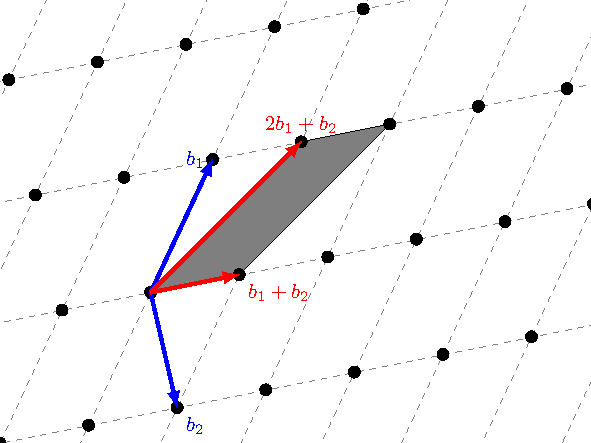
\includegraphics[width=0.625\textwidth]{figures/sections/section-2/lattice-structure-illustrative-example.pdf}
        \caption{An illustrative example of a lattice geometric group,\\ with a possible choice of 2 bases and 2 linear combinations of them.}
        \label{fig:lattice-structure-illustrative-example}
    \end{figure}
    
    \noindent Formally, given $n$-linearly independent vectors from a basis $\{\Vec{{b}_{1}}$, $\Vec{{b}_{2}}$, $\dots$, $\Vec{{b}_{n}}\}$ of ${\mathbb{R}}^{n}$, a lattice structure $\mathcal{L} \subset {\mathbb{R}^{n}}$ generated by them is a linear combination of the basis vectors $\Vec{b}$ and a given set of integer coefficients $x$, defined as follows:
    
    \begin{equation}
        \begin{split}     
            \mathcal{L}(\Vec{{b}_{1}}, \Vec{{b}_{2}}, \dots, \Vec{{b}_{n}}) & = \left\{ \sum_{i = 1}^{n} {c}_{i} \cdot \Vec{{b}_{i}}: {x}_{i} \in \mathbb{Z},\ \Vec{{b}_{i}} \in {\mathbb{R}}^{n} \right\} = \\
            & = {x}_{1} \cdot \Vec{{b}_{1}} + {x}_{2} \cdot \Vec{{b}_{2}} + \dots + {x}_{n} \cdot \Vec{{b}_{n}} = \\
            & = {x}_{1} \cdot
            \begin{pmatrix} 
                {b}_{(1, 1)} \\ {b}_{(1, 2)} \\ \vdots \\ {b}_{(1, n)}
            \end{pmatrix}
            + {x}_{2} \cdot
            \begin{pmatrix} 
                {b}_{(2, 1)} \\ {b}_{(2, 2)} \\ \vdots \\ {b}_{(2, n)}
            \end{pmatrix}
            + \dots + {x}_{n} \cdot
            \begin{pmatrix}
                {b}_{(n, 1)} \\ {b}_{(1, 2)} \\ \vdots \\ {b}_{(n, n)}
            \end{pmatrix}
        \end{split}
        \label{equ:lattice-structure-definition-1}
    \end{equation}
    \vspace{1ex}

    \newpage
    
    \noindent Indeed, the basis can be represented by the matrix $B = \begin{pmatrix} {b}_{1}, {b}_{2}, \dots, {b}_{n} \end{pmatrix}$, having the basis vectors ${b}_{i}$ as their columns, where $1 \leq i \leq n$. Using the matrix notation,\break a lattice structure generated by a matrix $B \in {\mathbb{R}}^{(n \times n)}$ can also be defined by\break $\mathcal{L}(B) = \{\ B \cdot x: B \in {\mathbb{R}}^{(n \times n)},\ x \in {\mathbb{Z}}^{n}\ \}$, using a matrix-multiplication as follows:

    \begin{equation}
        \begin{split}     
            \mathcal{L}(B) & = \left\{\ B \cdot x: B \in {\mathbb{R}}^{(n \times n)},\ x \in {\mathbb{Z}}^{n}\ \right\} = \\
            & = \begin{pmatrix}
                {b}_{(1, 1)} & {b}_{(2, 1)} & \dots & {b}_{(n, 1)} \\
                {b}_{(1, 2)} & {b}_{(2, 2)} & \dots & {b}_{(n, 2)} \\
                \vdots & \vdots & \ddots & \vdots \\
                {b}_{(1, n)} & {b}_{(2, n)} & \dots & {b}_{(n, n)}
            \end{pmatrix} \cdot
            \begin{pmatrix}
                {x}_{1} \\ {x}_{2} \\ \vdots \\ {x}_{n}
            \end{pmatrix} = \\
            & = \begin{pmatrix}
                {b}_{(1, 1)} \cdot {x}_{1} & + & {b}_{(2, 1)} \cdot {x}_{2} & + & \dots & + & {b}_{(n, 1)} \cdot {x}_{n} \\
                {b}_{(1, 2)} \cdot {x}_{1} & + & {b}_{(2, 2)} \cdot {x}_{2} & + & \dots & + & {b}_{(n, 2)} \cdot {x}_{n} \\
                \vdots & + & \vdots & + & \ddots & + & \vdots \\
                {b}_{(1, n)} \cdot {x}_{1} & + & {b}_{(2, n)} \cdot {x}_{2} & + & \dots & + & {b}_{(n, n)} \cdot {x}_{n}
            \end{pmatrix} = \\
            & = \begin{pmatrix}
                {b}_{(1, 1)} \cdot {x}_{1} \\
                {b}_{(1, 2)} \cdot {x}_{1} \\
                \vdots \\
                {b}_{(1, n)} \cdot {x}_{1}
            \end{pmatrix} + 
            \begin{pmatrix}
                {b}_{(2, 1)} \cdot {x}_{2} \\
                {b}_{(2, 2)} \cdot {x}_{2} \\
                \vdots \\
                {b}_{(2, n)} \cdot {x}_{2}
            \end{pmatrix} + \dots +
            \begin{pmatrix}
                {b}_{(n, 1)} \cdot {x}_{n} \\
                {b}_{(n, 2)} \cdot {x}_{n} \\
                \vdots \\
                {b}_{(n, n)} \cdot {x}_{n}
            \end{pmatrix} = \\
            & = \begin{pmatrix}
                {b}_{(1, 1)} \\
                {b}_{(1, 2)} \\
                \vdots \\
                {b}_{(1, n)}
            \end{pmatrix} \cdot {x}_{1} + 
            \begin{pmatrix}
                {b}_{(2, 1)} \\
                {b}_{(2, 2)} \\
                \vdots \\
                {b}_{(2, n)}
            \end{pmatrix} \cdot {x}_{2}+ \dots +
            \begin{pmatrix}
                {b}_{(n, 1)} \\
                {b}_{(n, 2)} \\
                \vdots \\
                {b}_{(n, n)}
            \end{pmatrix} \cdot {x}_{n} = \\
            & = {x}_{1} \cdot
            \begin{pmatrix} 
                {b}_{(1, 1)} \\ {b}_{(1, 2)} \\ \vdots \\ {b}_{(1, n)}
            \end{pmatrix}
            + {x}_{2} \cdot
            \begin{pmatrix} 
                {b}_{(2, 1)} \\ {b}_{(2, 2)} \\ \vdots \\ {b}_{(2, n)}
            \end{pmatrix}
            + \dots + {x}_{n} \cdot
            \begin{pmatrix}
                {b}_{(n, 1)} \\ {b}_{(1, 2)} \\ \vdots \\ {b}_{(n, n)}
            \end{pmatrix} = \\
            & = \mathcal{L}(\Vec{{b}_{1}}, \Vec{{b}_{2}}, \dots, \Vec{{b}_{n}}) \text{ (\ see \Cref{equ:lattice-structure-definition-1} )\ }
        \end{split}
        \label{equ:lattice-structure-definition-2}
    \end{equation}
    \vspace{1ex}

    \noindent Given a particular ($n \times n)$ unimodular matrix $U$, the bases $B$ and $B \cdot U$ generate the same lattice structure. In fact, we have the equality $\mathcal{L}(B) = \mathcal{L}(B')$ if and only if there is a unimodular matrix $U$ such that $B' = BU$. In particular, any lattice structure admits multiple bases, and this mathematical fact represents the core of many lattice-based cryptographic applications and primitives proposed. 

    The determinant of a lattice structure is given by the absolute value of the determinant of the basis matrix $B$, that is, $\det(\mathcal{L}(B)) = |\det(B)|$. The value of the determinant is independent of the choice of the basis and geometrically\break corresponds to the inverse of the density of the points of the lattice structure in ${\mathbb{R}}^{n}$. The dual of a lattice structure $\mathcal{L} \in {\mathbb{R}}^{n}$ denoted ${\mathcal{L}}^{*}$, is the lattice structure\break given by the set of all column $n$-vectors $\Vec{y} \in {\mathbb{R}}^{n}$ that satisfies $\langle \Vec{x}, \Vec{y} \rangle \in \mathbb{Z}$ for all\break column $n$-vectors $\Vec{x} \in \mathcal{L}$. Additionally, we can see that for any $B \in {\mathbb{R}}^{n}$,\break ${\mathcal{L}(B)}^{*} = \mathcal{L}({({B}^{-1})}^{T})$. Therefore, we also obtain the equality $\det({\mathcal{L}}^{*}) = \frac{1}{\det(\mathcal{L})}$. 
    
    Other lattice structures that are particularly important in Lattice-based Cryptography are $q$-ary (modular) lattice groups. These $q$-ary lattice groups are lattice structures $\mathcal{L}$ satisfying ${\mathbb{Z}}^{n} \subseteq \mathcal{L} \subseteq {\mathbb{Z}}^{n}$ for some prime integer $q$. In other words, we determine the membership of a vector $x \in \mathcal{L}$ by $x \mod q$. Then, we define such lattice groups in one-to-one correspondence with linear codes in ${\mathbb{Z}}^{n}_{q}$. Most constructions of Lattice-based Cryptography use $q$-ary (modular) lattice groups as their hard-on-average computational problem. Note that any lattice structure of integer elements $\mathcal{L} \subseteq {\mathbb{Z}}^{n}$ is a $q$-ary lattice group for some prime integer $q$. For example, whenever $q$ is an integer multiple of the determinant $\det(\mathcal{L})$. However, we are more concerned with $q$-ary (modular) lattice groups with a prime integer $q$ much smaller than $\det(\mathcal{L})$ in this specific configuration.

    \noindent Namely, given a matrix $X \in {Z}^{(m \times n)}_{q}$ for some integer numbers $q$, $m$, and $n$, we can mathematically define two $n$-dimensional $q$-ary lattice structures as follows:
    
    \begin{enumerate}
        \item ${\Lambda}_{q}(X) = \left\{ \Vec{y} \in {\mathbb{Z}}^{n}: \Vec{y} = {X}^{T} \times \Vec{s} \mod q\text{, for some } \Vec{s}\in {\mathbb{Z}}^{m} \right\}$;
        \item ${\Lambda}_{q}^{\perp}(X) = \left\{ \Vec{y} \in {\mathbb{Z}}^{n}: X \times \Vec{y} = \Vec{0} \mod q \right\}$.
    \end{enumerate}

    \noindent For the first case, we generate a specific $q$-ary lattice structure from the rows of matrix $X$. In the second case, a $q$-ary lattice structure contains all vectors being orthogonal modulo $q$ to the rows of matrix $X$. In other words, the $q$-ary lattice structure in the first case corresponds to the linear code generated by the rows of the matrix $X$. The one from the second case corresponds to the linear code whose parity check matrix is $X$. It follows since these lattice structures are dual to each other, up to normalization. Namely, we have the following equalities:
    
    \begin{enumerate}
        \item ${\Lambda}_{q}(X) = q \cdot {{\Lambda}_{q}^{\perp}(X)}^{*}$;
        \item ${\Lambda}_{q}^{\perp}(X) = q \cdot {{\Lambda}_{q}(X)}^{*}$.
    \end{enumerate}

    \noindent There are several ways to use lattice structures to build cryptographic primitives for (Classical) Post-Quantum Cryptography that are not always obvious. One first milestone in this line of research is a paper from Mikl\'{o}s Ajtai in 1996 \cite{ajtai:generating-hard-instances-lattice-problems:1996:06-2024,ajtai:shortest-vector-problem-l2-np-hard-randomized-reductions:1998:06-2024}, which defined the Short Integer Solution (SIS) Problem, and related its average\break case complexity to the worst-case hardness of finding short vectors in every\break integer lattice structure, giving novel cryptographic directions, proposing\break lattice-based One-Way Functions (OWFs) \cite{micciancio:generalized-compact-knapsacks-cyclic-lattices-efficient-one-way-functions:2007:06-2024} and Trapdoor Functions \cite{gentry-peikert-vaikuntanathan:trapdoors-hard-lattices-and-new-cryptographic-constructions:2007:06-2024}. Then, in the same year, Mikl\'{o}s Ajtai, jointly with Cynthia Dwork, presented a probabilistic public-key cryptosystem based on the hardness of the Shortest\break Vector Problem (SVP) \cite{ajtai-dwork:public-key-cryptosystem-with-worst-case-average-case-equivalence:1997:06-2024}. The security proof of this cryptosystem holds unless we can solve the worst-case of a well-known lattice problem in polynomial time.

    But before discussing this type of (Classical) Post-Quantum Cryptography in more detail, we first need to describe some mathematical problems that are computationally hard to solve, involving lattice structures at their core.
    
    \subsection{Lattice-based Problems}
    \label{subsec:lattice-based-problems}

    The constructions of cryptographic primitives for Lattice-based Cryptography use the presumed computational hardness of mathematical problems related to lattice structures, on which the SVP instances are the most popular ones and served as the inspiration for other similar lattice-based problems. In this case, we start with a lattice structure represented by an arbitrary basis given as an input for the problem, and the main goal is to output the shortest non-zero vector in it.\break

    \vspace{-2ex}
    
    \noindent Before entering the details of these problems, we need to introduce the notion of the shortest non-zero vector in a lattice structure $\mathcal{L}$ for a metric $\mathcal{M}$, given as:

    \begin{equation}
        \lambda(\mathcal{L}) = \min_{\Vec{\hat{v}}\ \in\ \mathcal{L} \setminus \{ \Vec{0} \} } {||\Vec{\hat{v}}||}_{\mathcal{M}}
        \label{equ:shortest-non-zero-vector-in-lattice}
    \end{equation}
    \vspace{1ex}

    \noindent
    
    \noindent Another important constant associated with a lattice structure $\mathcal{L}$ is the covering radius. We define a covering radius as the smallest radius $r$ for a family of closed spheres (or circles) with a center ${c}_{i}$, where $r > 0$, such that any $x \in {R}^{n}$ belong at least to one of those spheres (or circles), covering the entire vector space $\mathcal{V}$. In other words, we can define the covering radius $r$ of a lattice structure $\mathcal{L}$ generated from a basis $B$ as the maximum distance ${|| (\Vec{x} - \mathcal{L}(B) ) ||}_{\mathcal{M}}$, for a given metric $\mathcal{M}$, where the vector $\Vec{x}$ ranges over the linear span of the basis $B$. Thus, we can define the notion of covering radius $r$ of a lattice structure $\mathcal{L}$ as follows:

    \begin{equation}
        r = {\rho}_{M}(\mathcal{L}(B)) = \max_{\Vec{x}\ \in\ {\mathbb{R}}^{n}} {|| (\Vec{x} - \mathcal{L}(B) ) ||}_{\mathcal{M}}
        \label{equ:covering-radius-in-lattice}
    \end{equation}
    \vspace{1ex}

    \noindent Now, we can finally enumerate and briefly describe all the most currently known lattice-based mathematical and computational problems, in their \textit{exact} forms:

    \begin{enumerate}
        \item \textbf{\textit{Shortest Vector Problem}} (\textbf{\textit{SVP}}):
        \vspace{0.6ex}
        
        In the SVP instance, a basis of a vector space $\mathcal{V}$ and a metric $\mathcal{M}$, usually\break the Euclidean norm ${L}^{2}$, are given for a lattice structure $\mathcal{L}$ of size $n$ as input.\break Then, the goal is to find the shortest non-zero vector in the space vector $\mathcal{V}$\break from the starting point (origin) to another point on the ``grid-like'' structure using the directions provided by the basis vectors, as measured by $\mathcal{M}$, in the lattice structure $\mathcal{L}$. In other words, the solving algorithm should output a non-zero vector $\Vec{v}$, such that ${||\Vec{v}||}_{\mathcal{M}} = \lambda(\mathcal{L})$. This mathematical problem in its\break \textit{exact} form, i.e., without any form of approximation (considering $\gamma(n) = 1$),\break is only known to be NP-Hard for randomized reductions. By contrast, the corresponding mathematical problem, when considering the use of the\break uniform norm for the metric $\mathcal{M}$, is also known to be an NP-Hard problem.
        \vspace{2ex}

        \item \textbf{\textit{Closest Vector Problem}} (\textbf{\textit{CVP}}):
        \vspace{0.6ex}

        In the CVP instance, a basis of a vector space $\mathcal{V}$ and a metric $\mathcal{M}$, usually the Euclidean norm ${L}^{2}$, are given for a lattice structure $\mathcal{L}$ of size $n$ as input,\break together with a target vector $\Vec{v}$ in the vector space $\mathcal{V}$ but not necessarily in\break the lattice structure $\mathcal{L}$. The goal of the solving algorithm is to find the vector $\Vec{v'}$ in the lattice structure $\mathcal{L}$ closest to the given target vector $\Vec{v}$, as measured by the given metric $\mathcal{M}$. It is also known that any computational hardness of an SVP instance implies the same computational hardness for a CVP instance. On the other hand, CVP instances are widely regarded, in theory\break and practice, as considerably harder problems than SVP instances.
        \vspace{2ex}

        \item \textbf{\textit{Shortest Independent Vector Problem}} (\textbf{\textit{SIVP}}):
        \vspace{0.6ex}

        In the SIVP instance, a basis of a vector space $\mathcal{V}$ and a metric $\mathcal{M}$,\break usually the Euclidean norm ${L}^{2}$, are given for a lattice structure $\mathcal{L}$ of size $n$ as input. The goal of the solving algorithm is to find a set (i.e., a basis) of $n$\break linearly independent and short non-zero vectors $B' = \{ \Vec{{b'}_{1}}, \Vec{{b'}_{2}}, ..., \Vec{{b'}_{n}} \}$,\break so that ${\max}_{i} {||\Vec{{b'}_{i}}||}_{\mathcal{M}} \leq {\max}_{B} {||\Vec{{b}_{i}}||}_{\mathcal{M}}$, where $1 \leq i \leq n$ and $B = \{ \Vec{{b}_{1}}, \Vec{{b}_{2}}, ..., \Vec{{b}_{n}} \}$. In other words, for the best scenario, we seek to minimize the length of the longest vector in the original basis $B$ and find a new basis $B'$ that yields the same lattice structure $\mathcal{L}$. As far as we know, SIVP instances are also NP-Hard. However, they should generally be harder than SVP instances.
        \vspace{2ex}

        \item \textbf{\textit{Shortest Basis Problem}} (\textbf{\textit{SBP}}):
        \vspace{0.6ex}
        
        In the SBP instance, a basis of a vector space $\mathcal{V}$ and a metric $\mathcal{M}$, usually the Euclidean norm ${L}^{2}$, are given for a lattice structure $\mathcal{L}$ of size $n$ as input. The goal is to find an equivalent basis $B'$ that can serve as the new direction vectors for the lattice structure, such that the length of the longest vector in that basis is as short as possible. Essentially, the goal of the solving algorithm is to find the shortest possible set of direction vectors that still allow us to navigate the entire ``grid-like'' lattice structure. Despite the SBP instances not being explicitly considered NP-Hard problems in general, they are at least considered as hard as approximating the SVP or the CVP instances.
        \vspace{2ex}

        \item \textbf{\textit{Covering Radius Problem}} (\textbf{\textit{CRP}}):
        \vspace{0.6ex}

        In the CRP instance, a basis of a vector space $\mathcal{V}$, and a metric $\mathcal{M}$, usually the Euclidean norm ${L}^{2}$, are given for a lattice structure $\mathcal{L}$ of size $n$ as input. The goal is to find the smallest radius $r'$, defined as a rational number, such each circle (or sphere for higher-dimensions) of radius $r'$ centered around each point of the lattice structure $\mathcal{L}$ together can cover the entire space of the\break lattice structure without leaving any gaps. In other words, the goal of the solving algorithm is to find $r'$ such that $r = {\rho}_{\mathcal{M}}(\mathcal{L}(B)) \leq r$, where $r, r' \in \mathbb{Q}$ and ${\rho}_{\mathcal{M}}(\mathcal{L}(B))$ is the covering radius $\rho$ using the metric $\mathcal{M}$ that covers the entire space of the lattice structure $\mathcal{L}$ represented by the basis $B$. Usually,\break we consider the CRP instances NP-Hard because they involve finding a\break minimum radius for covering all possible points in a continuous (possibly\break infinite) space of a lattice structure while ensuring at least one circle\break (or sphere), centered at a lattice point with that radius, covers them all, which is currently considered to be computationally hard and intensive.
                
    \end{enumerate}

    \vspace{2ex}

    \noindent However, practical lattice-based public-key cryptosystems usually involve other approximate versions of the previously mentioned problems, which are outside\break the regime known to be NP-Hard. In addition, these NP-Hardness results only describe the worst-case asymptotic complexity of the problem, and we do not know how to apply this computational hardness directly to algebraically\break structured lattices. We can describe these approximate instances as follows:

    \begin{enumerate}
        \item \textbf{\textit{$\gamma$-Approximate Shortest Vector Problem}} (\textbf{\textit{$\gamma$-Approximate SVP}}):
        \vspace{0.6ex}
        
        In the $\gamma$-Approximate SVP instance, we consider the setup of the original SVP instance, but with an additional small approximation factor $\gamma$ that works as a \textit{relaxation} to the original \textit{exact} problem. Namely, we also consider a function defined as $\gamma = \gamma(n) \geq 1$ that depends on the dimension $n$ of the lattice structure $\mathcal{L}$. The goal of the solving algorithm is to find a non-zero lattice vector of a scaled length at most $\gamma \cdot \lambda(L)$, setting a lower bound for its shortest size that is greater than the one from the original \textit{exact} problem.
        \vspace{2ex}
        
        \item \textbf{\textit{$\gamma$-Approximate Closest Vector Problem}} (\textbf{\textit{$\gamma$-Approximate CVP}}):
        \vspace{0.6ex}

        In the $\gamma$-Approximate CVP instance, we consider the setup of the original CVP instance, but with an additional small approximation factor $\gamma$ that works as a \textit{relaxation} to the original \textit{exact} problem. Namely, we also consider a function defined as $\gamma = \gamma(n) \geq 1$ that depends on the dimension $n$ of the lattice structure $\mathcal{L}$. The goal of the solving algorithm is to find the vector $\Vec{v'}$ in the lattice structure $\mathcal{L}$ that is within a factor of $\gamma$ of the distance to the actual closest vector, as measured by the given metric $\mathcal{M}$, setting a lower bound for the distance to the closest vector that is greater than the one from the \textit{exact} problem. Here, $\gamma$ is a factor that represents how much further away the approximate solution vector $v'$ can be compared to the actual closest vector on the configuration of the original CVP instance.
        \vspace{2ex}
        
        \item \textbf{\textit{$\gamma$-Approximate Shortest Independent Vector Problem}}\\(\textbf{\textit{$\gamma$-Approximate SIVP}}):
        \vspace{0.6ex}
        
        In the $\gamma$-Approximate SIVP instance, we consider the setup of the original SIVP instance, but with an additional small approximation factor $\gamma$ that works as a \textit{relaxation} to the original \textit{exact} problem. Namely, we also consider\break a function defined as $\gamma = \gamma(n) \geq 1$ that depends on the dimension $n$ of the lattice structure $\mathcal{L}$. The goal of the solving algorithm is to find a set (i.e., a basis) of $n$ linearly independent and short non-zero vectors\break $B' = \{ \Vec{{b'}_{1}}, \Vec{{b'}_{2}}, ..., \Vec{{b'}_{n}} \}$, so that ${\max}_{i} {||\Vec{{b'}_{i}}||}_{\mathcal{M}} \leq \gamma \cdot {\max}_{B} {||\Vec{{b}_{i}}||}_{\mathcal{M}}$, where $1 \leq i \leq n$ and $B = \{ \Vec{{b}_{1}}, \Vec{{b}_{2}}, ..., \Vec{{b}_{n}} \}$. In other words, in the best scenario, we seek to minimize the length of the longest vector in the original basis $B$ and find a new basis $B'$, scaled at most by the given approximation factor $\gamma$, that yields the same lattice structure $\mathcal{L}$. Here, $\gamma$ is a factor representing how much longer the (approximated) linearly independent vectors can be compared to the shortest possible (original) linearly independent vectors. 
        \vspace{2ex}

        \newpage
        
        \item \textbf{\textit{$\gamma$-Approximate Shortest Basis Problem}} (\textbf{\textit{$\gamma$-Approximate SBP}}):
        \vspace{0.6ex}

        In the $\gamma$-Approximate SBP instance, we consider the setup of the original SBP instance, but with an additional small approximation factor $\gamma$ that works as a \textit{relaxation} to the original \textit{exact} problem. Namely, we also consider\break a function defined as $\gamma = \gamma(n) \geq 1$ that depends on the dimension $n$ of the lattice structure $\mathcal{L}$. The goal of the solving algorithm is to find a set (i.e., a basis) of direction vectors, scaled at most by the given approximation factor $\gamma$, as measured by the given metric $\mathcal{M}$, that still allow us to navigate the entire “grid-like” lattice structure. Here, $\gamma$ is a factor representing how much longer the (approximated) solution basis of direction vectors can be compared to the shortest possible (original) basis of direction vectors.
        \vspace{2ex}
        
        \item \textbf{\textit{$\gamma$-Approximate Covering Radius Problem (CRP)}}\\ (\textbf{\textit{$\gamma$-Approximate CRP}}):
        \vspace{0.6ex}

        In the $\gamma$-Approximate CRP instance, we consider the setup of the original CRP instance, but with an additional small approximation factor $\gamma$ that works as a \textit{relaxation} to the original \textit{exact} problem. Namely, we also consider\break a function defined as $\gamma = \gamma(n) \geq 1$ that depends on the dimension $n$ of the lattice structure $\mathcal{L}$. The goal of the solving algorithm is to find the smallest radius scaled at most by the given approximation factor $\gamma$, as measured by the given metric $\mathcal{M}$, such each circle (or sphere for higher-dimensions) with that scaled radius centered around each point of the lattice structure together can cover the entire space of the lattice structure without leaving any gaps. Here, $\gamma$ is a factor representing how much longer the (approximated) solution\break radius of the circle or sphere can be compared to the shortest (original) one.
        
    \end{enumerate}
    
    \subsection{Algorithms for Lattice-based Problems}
    \label{subsec:algorithms-for-lattice-based-problems}

    Now that we already addressed some of the most popular lattice-based problems used as the basis of Lattice-based Cryptography, we can introduce some of the currently known best algorithms for solving such mathematical problems.

    \subsubsection{Lattice's Basis Reduction Algorithms}
    \label{subsubsec:lattice-basis-reduction-algorithms}

    \begin{enumerate}
        \item \textbf{\textit{Lenstra-Lenstra-Lov\'{a}sz}} (\textbf{\textit{LLL}}) \textbf{\textit{Algorithm}}:
        \vspace{0.6ex}

        The Lenstra-Lenstra-Lovasz (LLL) algorithm \cite{lenstra-lenstra-lovasz:factoring-polynomials-with-rational-coefficients:1982:06-2024} is a polynomial time\break algorithm for lattice basis reduction invented jointly by Arjen Lenstra,\break Hendrik Lenstra, and L\'{a}szl\'{o} Lov\'{a}sz in 1982. Given a basis $B = \{ {b}_{1}, {b}_{2}, ..., {b}_{d} \}$ of size $d$ with $n$-dimensional vectors for a lattice structure $\mathcal{L}$, with $d \leq n$, this\break reduction algorithm computes a short and nearly orthogonal lattice basis,\break known as an LLL-reduced lattice basis instance. The algorithm starts by, given the basis $B$, defining the Gram-Schmidt process orthogonal basis\break ${B}^{*} = \{ {b}^{*}_{1}, {b}^{*}_{2}, ..., {b}^{*}_{d} \}$ and the Gram-Schmidt coefficients ${\mu}_{i,j} = \frac{ \left\langle {b}_{i},{b}^{*}_{j} \right\rangle }{ \left\langle {b}^{*}_{j},{b}^{*}_{j} \right\rangle }$\footnote{In this context, $\left\langle m, n \right\rangle$ represents the inner product between $m$ and $n$.}, for\break\newpage any $1 \leq j < i \leq d$. Then, the basis $B$ is LLL-reduced if there exists a real parameter $\delta \in\ ]0.25,1]$, such that the following enumerated conditions hold:
        \begin{enumerate}
            \item For $1 \leq j < i \leq d: |{\mu}_{i,j}| \leq 0.5$. By definition, this property guarantees\break the length reduction of the ordered basis. \textbf{(Size-reduced condition)}
            \item For $k = 2, 3, ..., d: \delta \times {||{b}^{*}_{(k - 1)}||}^{2} \leq {||{b}^{*}_{k}||}^{2} + {\mu}^{2}_{k,(k - 1)} \times {||{b}^{*}_{(k - 1)}||}^{2}$,\break where $d \in \mathbb{Z}$, $\delta \in \mathbb{R}$, and $\delta \in\ ]0.25,1]$. \textbf{(Lov\'{a}sz condition)}
        \end{enumerate}
        \vspace{2ex}
        
        Here, estimating the value of the $\delta$ parameter, we can conclude how well we are reducing the lattice basis, where greater delta values lead to better reductions of the lattice basis. Initially, Arjen Lenstra, Hendrik Lenstra, and L\'{a}szl\'{o} Lov\'{a}sz demonstrated the LLL-reduction algorithm for $\delta = \frac{3}{4}$. It is important to note that although LLL-reduction is well-defined for $\delta = 1$, the LLL algorithm only guarantees a polynomial-time complexity for $\delta \in ]0.25, 1[$.

        \vspace{2ex}
        
        In this context, the Gram-Schmidt orthogonalized vectors ${b}^{*}_{j}$ are defined as:
        
        $$ {b}^{*}_{j} = {b}_{j}\ - \sum_{i = 1}^{(j - 1)} {\mu}_{j,i} \times {b}^{*}_{i},\ \mathrm{for}\ j = 2, ..., d,\ \mathrm{and\ where}\ {b}^{*}_{1} = {b}_{1} $$

        \vspace{2ex}
        
        There is no known efficient algorithm to compute a lattice basis in which the basis vectors are as short as possible for lattice structures of dimensions greater than $4$. However, an LLL-reduced lattice basis is nearly as short as possible, in the sense that there are absolute bounds ${c}_{i} > 1$ such that the ${i}^{th}$ reduced basis vector is no more than ${c}_{i}$ times as long as the respective shortest ${i}^{th}$ basis vector in the lattice structure, with $1 \leq i \leq d$ and $d \in \mathbb{Z}$.

        We can describe the general LLL algorithm by defining also two auxiliary\break sub-routines, the Nearest Plane Algorithm \cite{babai:lovasz-lattice-reduction-and-nearest-lattice-point-problem:1986:06-2024} and the Lattice Basis Size\break Reduction Algorithm \cite{lenstra-lenstra-lovasz:factoring-polynomials-with-rational-coefficients:1982:06-2024}. After correctly defining these two sub-routines, it is easier to build the general LLL algorithm since it uses them both.

        These two sub-routines jointly select the hyperplane closest to the target vector $c = \left\lfloor \frac{ \langle t, {b}^{*}_{n} \rangle }{ {|| {b}^{*}_{n} ||}^{2} } \right\rceil$, and recursively search for a lattice point in $c \times {b}_{k} + \mathcal{L}(B')$ close to the target vector $t$, or equivalently, a lattice point in the lower dimensional sub-lattice $\mathcal{L}(B')$ close to $(t - c \times {b}_{k})$. The base case is when the rank of the lattice is reduced to $0$ and the only possible output is also $0$.

        The LLL algorithm for lattice basis reduction, calculates a nearly orthogonal reduced lattice basis (also called LLL-reduced basis) in a complexity time of $\mathcal{O}\left({d}^{5} \times n \times \log^{3}(L)\right)$, where $L$ is the largest length of ${b}_{i}$ under the Euclidean norm, that is, $L = \max\left( {||{b}_{i}||}_{2} \right) = \max\left( {||{b}_{1}||}_{2}, ..., {||{b}_{d}||}_{2} \right)$, for $1 \leq i \leq d$.

        Additionally, the LLL algorithm has also found numerous other applications\break in cryptanalysis of public-key encryption schemes and cryptosystems, such as Naccache–Stern Knapsack \cite{naccache-stern:new-public-key-cryptosystem-based-higher-residues:1998:06-2024}, RSA \cite{rivest-shamir-adleman:method-digital-signatures-and-public-key-cryptosystems:1978:06-2024} (with particular settings), or Nth Degree Truncated Polynomial Ring Units - Encrypt (NTRUEncrypt) \cite{hoffstein-pipher-silverman:ntru-ring-based-public-key-cryptosystem:1998:06-2024}.        
    
        \clearpage
        
        The pseudo-code for the sub-routine of the Nearest Plane Algorithm that, given an input lattice basis $B$ and a target vector $t$, outputs a lattice point $v \in \mathcal{L}(B)$ such that $\frac{ \left\langle t -  v, {b}^{*}_{i}\right\rangle }{{|| {b}_{i}^{*} ||}^{2} } \in \left[-\frac{1}{2}, \frac{1}{2}\right[$ for all $i = 1, ..., d$, is given as follows:

        \vspace{-2ex}
        \begin{algorithm}
            \caption{\texorpdfstring{\texttt{NearestPlane}}\/: Nearest Plane Algorithm}
            \label{subrou:nearest-plane-algorithm}
            
            \textbf{Input:} $ (B, t) $\\
            \textbf{Output:} $ v $
            
            \begin{algorithmic}[1]
                \Ensure $B \in {\mathbb{R}}^{n \times d},\ t \in {\mathbb{R}}^{n},\ v \in \mathcal{L}(B)$
            
                \vspace{2ex}

                \If{n = 0}
                    \State \Return 0
                \Else
                    \State ${B}^{*} \gets \texttt{GramSchmidt}(B)$
                    \State $c \gets \left\lfloor \frac{ \langle t, {b}^{*}_{n} \rangle }{ {|| {b}^{*}_{n} ||}^{2} } \right\rceil$
                    \State \Return $c \times {b}_{n} + \texttt{NearestPlane}\left([{b}_{1}, ..., {b}_{(d - 1)}], t - (c \times {b}_{d})\right)$
                \EndIf
            \end{algorithmic}
        \end{algorithm}
        
        The pseudo-code for the sub-routine of the Lattice Basis Size Reduction Algorithm that, given an input lattice basis $B$, outputs the same lattice basis $B$ but with its size reduced, is given in detail as presented below:

        \vspace{-2ex}
        \begin{algorithm}
            \caption{\texorpdfstring{\texttt{SizeReduction}}\/: Lattice Basis Size Reduction Algorithm}
            \label{subrou:lattice-basis-size-reduction-algorithm}
            
            \textbf{Input:} $ B $\\
            \textbf{Output:} $ B $
            
            \begin{algorithmic}[1]
                \Ensure $B \in {\mathbb{R}}^{n \times d}$
            
                \vspace{2ex}

                \For{$i = 2$ to $n$}
                    \State $x \gets \texttt{NearestPlane}(B, {b}_{i} - {b}^{*}_{i})$
                    \State ${b}_{i} \gets {b}_{i} - B \times x$
                \EndFor
                \State \Return $B$
            \end{algorithmic}
        \end{algorithm}

        In the context of the LLL algorithm for lattice basis reduction, we need to define ${\pi}_{j}(b)$ as the projection of the bases vector $b$ onto the orthogonal complement of the sub-space spanned by the first $(j - 1)$ basis vectors. This projection is crucial for the \texttt{SizeReduction} step and to maintain the Lovasz condition, which together ensure the generation of a reduced and nearly orthogonal lattice basis. The projection ${\pi}_{j}(b)$ is given by removing the components of $b$ that lie in the direction of ${b}^{*}_{[1,(j - 1)]} = ({b}^{*}_{1}, ..., {b}^{*}_{(j - 1)})$, and therefore, we can defined it mathematically as presented below:

        $$ {\pi}_{j}(b) = b\ - \sum_{i = 1}^{(j - 1)} {\mu}_{j,i} \times {b}^{*}_{i} $$

        \clearpage
        
        The pseudo-code for the sub-routine of the LLL Basis Reduction Algorithm that, given an input lattice basis $B$ and a real parameter $\delta$, outputs the same lattice basis $B$ but reduced by the LLL algorithm, is presented below:

        \vspace{-2ex}
        \floatname{algorithm}{Algorithm}
        \setcounter{algorithm}{0}
        \begin{algorithm}
            \caption{\texorpdfstring{\texttt{LLL}}\/: LLL Lattice Basis Reduction Algorithm}
            \label{subrou:lll-lattice-basis-reduction-algorithm}
            
            \textbf{Input:} $ (B,\delta) $\\
            \textbf{Output:} $ B $
            
            \begin{algorithmic}[1]
                \Ensure $B \in {\mathbb{R}}^{n \times d},\ \delta \in \mathbb{R},\ \delta \in\ ]0.25, 1]$
            
                \vspace{2ex}

                \State $B \gets \texttt{SizeReduction}(B)$
                \For{$i = 1$ to $(d - 1)$}
                    \If{$\delta \times {|| {\pi}_{i}({b}_{i}) ||}^{2} > {|| {\pi}_{i}({b}_{(i + 1)}) ||}^{2}$}
                        \State $\texttt{swap}({b}_{i},{b}_{(i + 1)})$
                        \State \Return $\texttt{LLL}(B,\delta)$
                    \Else
                        \State \Return $B$
                    \EndIf
                \EndFor
            \end{algorithmic}
        \end{algorithm}
        
        
        \item \textbf{\textit{Block Korkine-Zolotarev}} (\textbf{\textit{BKZ}}) \textbf{\textit{Algorithm}}:
        \vspace{0.6ex}

        Before describing the Block Korkine-Zolotarev (BKZ) algorithm \cite{yasuda:survey-solving-svp-algorithms-recent-strategies-solving-svp-challenge:2021:06-2024} for\break lattice basis reduction, we need to introduce the Korkine-Zolotarev (KZ) algorithm \cite{korkine-zolotarev:sur-les-formes-quadratiques-positives:1877:06-2024}, which is also known as Hermite–Korkine–Zolotarev (HKZ) algorithm. For lattice structures defined in ${R}^{n}$, the KZ algorithm yields a\break lattice basis with orthogonality defect at most ${n}^{n}$ steps, unlike the ${2}^{\left(\frac{{n}^{2}}{2}\right)}$ bound for the steps of the LLL algorithm \cite{lenstra-lenstra-lovasz:factoring-polynomials-with-rational-coefficients:1982:06-2024}. The KZ algorithm \cite{korkine-zolotarev:sur-les-formes-quadratiques-positives:1877:06-2024} has\break an exponential complexity when compared to the polynomial complexity of the LLL algorithm. However, we may prefer the KZ algorithm for solving\break multiple CVP instances in the same lattice structure, where it can be more\break efficient. First, Aleksandr Korkine and Yegor Zolotarev defined a KZ-reduced lattice basis in 1877 as a strengthened version of the Hermite-reduction \cite{korkine-zolotarev:sur-les-formes-quadratiques-positives:1877:06-2024}. Later, in 1983, Ravi Kannan proposed the first algorithm to construct a KZ-reduced lattice basis \cite{kannan:improved-algorithms-integer-programming-related-lattice-problems:1983:06-2024}. Then, Masaya Yasuda introduced the BKZ\break algorithm in 1987 \cite{yasuda:survey-solving-svp-algorithms-recent-strategies-solving-svp-challenge:2021:06-2024}, and improved later by Claus-Peter Schnorr and Martin Euchner in 1991 \cite{schnorr-euchner:lattice-basis-reduction-improved-practical-algorithms-and-solving-subset-sum-problems:1994:06-2024}, as some refined versions of the algorithm.

        Namely, the BKZ algorithm provides a more scalable and practical approach for lattice basis reduction by generalizing the (original) KZ algorithm to blocks of vectors instead of single ones. The BKZ algorithm applies the KZ algorithm to each block of vectors, thereby achieving stronger lattice basis reductions than the LLL algorithm while being more efficient than a (full) lattice basis reduction from the KZ algorithm. The quality of the lattice basis reduction depends on the block size parameter, usually denoted as $\beta$. Namely, $\beta$ offers a trade-off between accuracy and performance in a sense that larger block sizes yield better reductions but require more computational effort.

        \clearpage

        There are several variants of the BKZ algorithm for lattice basis reduction, but in this report, we will follow the one given by Claus-Peter Schnorr and Martin Euchner \cite{schnorr-euchner:lattice-basis-reduction-improved-practical-algorithms-and-solving-subset-sum-problems:1994:06-2024}. The pseudo-code of this BKZ algorithm variant is:

        \vspace{-2ex}
        \floatname{algorithm}{Algorithm}
        \begin{algorithm}
            \caption{\texorpdfstring{\texttt{BKZ}}\/: BKZ Lattice Basis Reduction Algorithm\\\phantom{...............................}(Schnorr-Euchner's variant)}
            \label{subrou:bkz-lattice-basis-reduction-algorithm}
            
            \textbf{Input:} $ (B,\beta,\gamma) $\\
            \textbf{Output:} $ B $
            
            \begin{algorithmic}[1]
                \Ensure $B \in {\mathbb{R}}^{n \times d},\ \beta \in \mathbb{Z},\ \beta \in [2,d],\ \gamma \in \mathbb{R},\ \gamma \in [1, 2]$
            
                \vspace{2ex}

                \State $z \gets 0$
                \State $j \gets 0$
                \State $B \gets \texttt{LLL}\left(B,\frac{1}{\gamma}\right)$
                \While{$z < (d - 1)$}
                    \State $j \gets (j \mod (d - 1)) + 1$
                    \State ${d}_{j} \gets \min\left( (j + \beta - 1), d \right)$
                    \State $h \gets \min\left( (j + \beta), d \right)$
                    \State $\mathrm{A} = ({\alpha}_{j}, ..., {\alpha}_{{d}_{j}}) \gets \texttt{Enumerate}\left( \mathcal{L}({B}_{[j, {d}_{j}]}) \right)$
                    \If{$|| {\pi}_{j}(b) || = {\lambda}_{1}\left( L({B}_{[j,{d}_{j}]}) \right)$}
                        \State $b = \sum_{i = j}^{{d}_{j}} {\alpha}_{i} \times {b}_{i}$
                    \EndIf
                    \If{$ {|| {b}^{*}_{j} ||}^{2} > \gamma \times { || {\pi}_{j}(b) || }^{2} $}
                        \State $z \gets 0$
                        \State $B' \gets {B}_{[1, (j - 1)]} \cup B \cup {B}_{[j, h]} = ({b}_{1}, ..., {b}_{(j - 1)}, b, {b}_{j}, ..., {b}_{h})$
                        \State $B \gets \texttt{LLL}\left(B',\frac{1}{\gamma}\right)$
                    \Else
                        \State $z \gets (z + 1)$
                        \State $B'' \gets {B}_{[1, h]} = ({b}_{1}, ..., {b}_{h})$
                        \State $B \gets \texttt{LLL}\left(B'',0.99\right)$
                    \EndIf
                \EndWhile
                \State \Return $B$
            \end{algorithmic}
        \end{algorithm}
        \vspace{-2ex}

        Here, the \texttt{Enumerate} step in the BKZ algorithm for lattice basis reduction is a local search procedure within a block of lattice basis vectors, aiming to find the shorter lattice basis vectors by systematically exploring combinations of the former ones. This intermediate enumeration step is computationally demanding but crucial for achieving high-quality lattice basis reduction.

        Namely, the \texttt{Enumerate} step aims to find a shorter lattice basis vector\break $\mathbb{A} = ({\alpha}_{j}, ..., {\alpha}_{{d}_{j}}) \in {\mathbb{Z}}^{({d}_{j} - j + 1)}$ for $\mathcal{L}\left({B}_{[j, {d}_{j}]}\right)$. Additionally, ${\lambda}_{1}\left( L({B}_{[j,{d}_{j}]}) \right)$ represents the length of the shortest non-zero lattice basis vector in a lattice structure and a new bases vector $b = \sum_{i = j}^{{d}_{j}} {\alpha}_{i} \times {b}_{i}$ is computed such that $|| {\pi}_{j}(b) || = {\lambda}_{1}\left( L({B}_{[j,{d}_{j}]}) \right)$. Right after the step $20$ of the pseudo-code for the BKZ algorithm, ${B}_{[jm {d}_{j}]}$ may no longer be $\gamma$-SVP-reduced due to the calls to the LLL algorithm for lattice basis reduction at the steps $15$ and $19$. Finally,\break it is ``folklore'' in practice to allow a relaxation factor $\gamma = 1$, and it is\break recommended to run the LLL algorithm with $\frac{1}{\gamma} = 0.99$ at steps $3$ and $15$.
    \end{enumerate}
    

    \subsubsection{Shortest Vector Problem (SVP) Algorithms}
    \label{subsubsec:shortest-vector-problem-algorithms}

    Regarding the specific algorithms for solving the Shortest Vector Problem (SVP), there are two general types of algorithms: the Exact Algorithms to find exact solutions and the Approximation Algorithms to find approximated solutions.

    \vspace{2ex}
    
    \noindent For the Exact Algorithms, there are three main approaches to the exact solution of SVP instances in $d$-dimensional lattice structures, enumerated as follows:

    \begin{enumerate}
        \item \textbf{\textit{Enumeration Algorithms}}:
        \vspace{0.6ex}

        The Enumeration Algorithms for lattices \cite{fincke-pohst:improved-methods-calculating-vectors-short-length-lattice-including-complexity-analysis:1985:06-2024,kannan:minkowski-convex-body-theorem-and-integer-programming:1987:06-2024,hanrot-stehle:improved-analysis-kannan-shortest-lattice-vector-algorithms:2007:06-2024,pujol-stehle:rigorous-and-efficient-short-lattice-vectors-enumeration:2008:06-2024,micciancio-walter:fast-lattice-point-enumeration-minimal-overhead:2015:06-2024} are methods to list all the elements of a lattice structure or to find certain elements that meet specific\break criteria defined \textit{a priori}. The common proceeding of an Enumeration\break Algorithm for lattice structures starts with a pre-processing step, usually through a lattice basis reduction algorithm, such as the LLL algorithm, to make the lattice basis vectors shorter and closer to orthogonal, followed by the setting up of the initial parameters for a (geometric) search space and then starts the enumeration from the origin or a specified starting point,\break using a search or optimization algorithm to explore the points of the lattice\break structure, such as Depth-First Search (DFS) and Breadth-First Search (BFS), or even Branch-and-Bound algorithms. At each step of the search or\break optimization, the algorithm performs pruning using geometric insights based\break on the search space to eliminate infeasible regions or calculating bounds to determine if further exploration along a branch is necessary. Finally, the\break algorithm stores or outputs the points of the lattice structure that meet the criteria (e.g., points within a certain distance from the origin/starting point).
        
        These Enumeration Algorithms for lattice structures have super-exponential running time ${d}^{O(d)}$ but have the advantage of being deterministic and using\break only polynomial space. These algorithms are standard techniques to solve SVP and CVP instances on arbitrary lattice structures by systematically enumerating all lattice points in a bounded region of space (typically\break a $d$-dimensional parallelepiped or ellipsoid). Interest in Enumeration\break techniques for lattice structures is due to their low memory requirements\break (linear in the lattice structures of dimension $d$) and excellent practical\break performance in moderately low dimensions. Within the class of polynomial space algorithms, enumeration methods currently provide the asymptotically\break fastest algorithms to find exact solutions to SVP and CVP, both in theory\break and practice, with a worst-case time complexity of ${d}^{O(d)}$. Sieving Algorithms\break \cite{ajtai-kumar-sivakumar:sieve-algorithm-shortest-lattice-vector-problem:2001:06-2024,nguyen-vidick:sieve-algorithms-shortest-vector-problem-practical:2008:06-2024,micciancio-voulgaris:faster-exponential-time-algorithms-shortest-vector-problem:2010:06-2024,hanrot-pujol-stehle:algorithms-shortest-and-closest-lattice-vector-problems:2011:06-2024} and Voronoi Cell Computation Algorithms \cite{sommer-feder-shalvi:finding-closest-lattice-point-interactive-slicing:2009:06-2024,micciancio-voulgaris:deterministic-single-exponential-time-algorithm-most-lattice-problems-based-voronoi-cell-computations:2013:06-2024,mckilliam-grant-clarkson:finding-closest-point-lattice-voronoi-first-kind:2014:06-2024,dadush-bonifas:short-paths-voronoi-graph-and-closest-vector-problem-with-preprocessing:2015:06-2024} provide\break theoretically faster solutions to SVP and CVP instances but at the cost of\break using exponential space and occasionally randomness. Moreover, several\break optimizations and heuristics have been developed over the years, making this\break approach the most attractive in practice for moderately small dimensions.
        
        \vspace{2ex}
        \item \textbf{\textit{Voronoi Cell Computation Algorithms}}:
        \vspace{0.6ex}

        The Voronoi Cell Computation Algorithms \cite{sommer-feder-shalvi:finding-closest-lattice-point-interactive-slicing:2009:06-2024,micciancio-voulgaris:deterministic-single-exponential-time-algorithm-most-lattice-problems-based-voronoi-cell-computations:2013:06-2024,mckilliam-grant-clarkson:finding-closest-point-lattice-voronoi-first-kind:2014:06-2024,dadush-bonifas:short-paths-voronoi-graph-and-closest-vector-problem-with-preprocessing:2015:06-2024} for lattice structures\break involve determining the regions of a vector space closest to each point of the lattice structure. The Voronoi Cell of a lattice point is the set of all points in the vector space closer to that lattice point than any other point of the same lattice structure. Generally, there are two main approaches for this type of\break algorithm: Direct Geometric Construction (via Voronoi Diagram Generation\break \cite{voronoi:nouvelles-applications-parametres-continus-theorie-formes-quadratiques:1908:06-2024}) and Delaunay Triangulation \cite{delaunay:sur-la-sphere-vide:1934:06-2024} (using dual lattice structures).

        The Direct Voronoi Cell Computation Algorithms via Voronoi Diagrams usually start with a set of seed points on the lattice structure, and for each pair of seed points, compute the perpendicular bisector (a line equidistant from the two points for two-dimensional spaces and a hyperplane for higher dimensional spaces). For each of the perpendicular bisectors, the algorithm computes the respective intersections to find the vertices of the Voronoi Cells. Finally, those vertices are connected to form the edges and faces of the Voronoi Cells. Each Voronoi Cell corresponds to one seed point and contains all points of the lattice structure closer to it than any other seed point. This approach may require handling the boundaries of the vector space appropriately. For an infinite lattice structure, it might be practical to consider periodic boundary conditions or a large enough bounding box.

        On the other hand, the Indirect Voronoi Cell Computation Algorithms via Delaunay Triangulation usually also start with a set of seed points on the lattice structure, and for the set of seed points, construct the Delaunay Triangulation. Here, the Delaunay Triangulation means forming triangles such that no lattice point is inside the circumcircle of any triangle for a two-dimensional space or forming simplices such that no lattice point is inside the sphere of any simplex for a higher-dimensional space. Next, for each simplex in the Delaunay Triangulation, the algorithm computes its circumcenter (i.e., the center of the circumcircle or sphere). The algorithm uses these circumcenters as vertices of the Voronoi Cells. The edges and faces of the Voronoi Cells correspond to the adjacency of the simplices in the Delaunay Triangulation. Then, the algorithm connects the circumcenters to form the edges and faces of the Voronoi Cells. Each Voronoi Cell corresponds to one seed point in the lattice structure. Similar to the Direct Voronoi Cell Computation Algorithms, handling boundaries might be appropriate.

        This approach improves the running time for solving SVP instances and many other lattice problems to $O({2}^{{2}^{d}})$, using exponential space $O({2}^{n})$. These are currently the asymptotically fastest known deterministic algorithms for solving SVP, but they are not competitive in practice with other approaches.

        \vspace{2ex}
        \item \textbf{\textit{Sieving Algorithms}}:
        \vspace{0.6ex}

        The Sieving Algorithms \cite{ajtai-kumar-sivakumar:sieve-algorithm-shortest-lattice-vector-problem:2001:06-2024,nguyen-vidick:sieve-algorithms-shortest-vector-problem-practical:2008:06-2024,micciancio-voulgaris:faster-exponential-time-algorithms-shortest-vector-problem:2010:06-2024,hanrot-pujol-stehle:algorithms-shortest-and-closest-lattice-vector-problems:2011:06-2024} for lattice groups are advanced techniques\break that work by iteratively refining a set of candidate lattice vectors. This\break refining procedure is done by sieving out longer vectors and keeping shorter ones until finding the optimal vector in the lattice structure. These\break algorithms usually start by reducing the lattice basis using techniques like LLL or BKZ algorithms to turn the lattice basis vectors shorter and more\break orthogonal, simplifying the subsequent sieving process. These algorithms then generate a set of random lattice vectors through random combinations\break of the lattice basis vectors or by sampling from a Gaussian distribution\break centered at the origin. Next, for each pair of random lattice vectors, these Sieving Algorithms compute a new difference vector between those vectors, and if this new random lattice vector is shorter than both previous vectors, replace one of those vectors with the new one. These algorithms perform this pairwise reduction process iteratively, and during each iteration, we expect the set of random lattice vectors to contain shorter vectors as the reductions progress. This step pairwise reduction is executed while checking convergence by monitoring the length of the shortest vector in the set. If the length stops decreasing significantly between iterations, the algorithm has likely converged to a solution. We can optimize these algorithms by\break restricting the set of random lattice vectors to lie within a specific bounding volume, reducing the number of vectors considered at each step, speeding up the convergence, and parallelizing the pairwise reduction step. Additionally,\break we can employ hashing and compression techniques to quickly find and\break compare lattice vectors of high dimensions in the pairwise reduction step.

        These Sieving Algorithms improve the asymptotic running time of traditional Enumeration Algorithms, reducing the dependency of the running time on the dimension of the lattice structure from ${d}^{O(d)}$ to single exponential ${2}^{(c \times d)}$ for some constant $c = O(1)$. These algorithms achieve this improvement at the cost of introducing randomization processes and using exponential space.
        
    \end{enumerate}

    \vspace{2ex}
    
    \noindent The Approximation Algorithms for SVP instances are usually based on lattice basis reduction techniques, such as the LLL and BKZ algorithms, and achieve approximation factors for the solution as small as ${2}^{O(\log(d)/\log(\log(d)))} = {d}^{O(1)}$.
    
    \subsubsection{Closest Vector Problem (CVP) Algorithms}
    \label{subsubsec:closest-vector-problem-algorithms}
    
    Regarding the specific algorithms for solving the Closest Vector Problem (CVP), there are two main approaches: the Enumeration Algorithms to find exact\break solutions and Babai's Nearest Plane Algorithm to find approximated solutions.

    \begin{enumerate}
        \item \textbf{\textit{Enumeration Algorithms}}:
        \vspace{0.6ex}
        
        The Enumeration Algorithms \cite{fincke-pohst:improved-methods-calculating-vectors-short-length-lattice-including-complexity-analysis:1985:06-2024,kannan:minkowski-convex-body-theorem-and-integer-programming:1987:06-2024,hanrot-stehle:improved-analysis-kannan-shortest-lattice-vector-algorithms:2007:06-2024,pujol-stehle:rigorous-and-efficient-short-lattice-vectors-enumeration:2008:06-2024,micciancio-walter:fast-lattice-point-enumeration-minimal-overhead:2015:06-2024} for CVP instances are very similar to the ones for solving SVP instances. These algorithms list all the elements of a lattice structure or find certain elements that meet criteria defined \textit{a priori}. The standard procedure involves a pre-processing step, through a lattice basis reduction, a setup of the initial parameters for a search space, and a search or optimization step from the origin or a starting point. At the end, the algorithm stores/outputs the points of the lattice structure meeting the criteria (e.g., points within a certain distance from the starting point).
        
        These Enumeration Algorithms for lattice structures have super-exponential running time ${d}^{O(d)}$ but have the advantage of being deterministic and using\break only polynomial space. These algorithms are standard techniques to solve CVP instances on arbitrary lattice structures by systematically enumerating all lattice points in a bounded region of space. Within the class of polynomial\break space algorithms, enumeration methods currently provide the asymptotically\break fastest algorithms to find exact solutions to CVP, with a worst-case time complexity of ${d}^{O(d)}$. Other algorithms provide theoretically faster solutions to CVP instances but at the cost of using exponential space and randomness.

        \vspace{2ex}
        \item \textbf{\textit{Babai's Nearest Plane Algorithm}}:
        \vspace{0.6ex}

        The Babai's Nearest Plane Algorithm \cite{babai:lovasz-lattice-reduction-and-nearest-lattice-point-problem:1986:06-2024} (also known as Babai's Nearest\break Hyperplane Algorithm) is a technique used to find an approximate solution\break to CVP instances in lattice-based theory, introduced by L\'{a}szl\'{o} Babai in 1986. This algorithm leverages the Gram-Schmidt Orthogonalization process\break to simplify the problem and provide an approximate solution to the problem.

        The algorithm receives the lattice basis and a target point in the vector space as inputs. Initially, the algorithm commonly starts by performing some\break pre-processing through the Gram-Schmidt procedure on the basis vectors to obtain an orthogonal basis. Next, the algorithm projects the target point onto the orthogonal vector of each of the lattice basis vectors, starting from the last one. Then, the algorithm determines the nearest integer coefficients for all lattice bases iteratively, such the product between that coefficient and the respective basis vector is close to the projection computed before,\break subtracting that multiplication result from the target vector and updating its value. Finally, the Babai's Nearest Plane Algorithm uses all the integer\break coefficients obtained through the previous iterative projection step to\break construct the approximate closest vector in the lattice ``grid-like'' structure.
        
        In summary, this algorithm systematically approximates the closest point on a lattice structure to a given target point by orthogonalizing the ``grid-like'' structure and iteratively adjusting the target point using projections.
    \end{enumerate}

    \subsubsection{Quantum Algorithms}
    \label{subsubsec:quantum-algorithms}

    A different approach for solving lattice-based problems is to leverage some of the principles and fundamentals of Quantum Computing to develop Quantum\break Algorithms that potentially provide significant speedups over classical ones.    
    
    \begin{enumerate}
        
        \item \textbf{\textit{Quantum Lattice Basis Reduction Algorithms}}:
        \vspace{0.6ex}

        The Quantum Lattice Basis Reduction Algorithms \cite{ludwig:faster-lattice-reduction-method-using-quantum-search:2003:06-2024,ambainis-kempe:quantum-lovasz-local-lemma:2012:06-2024,tiepelt-szepieniec:quantum-lll-application-mersenne-number-cryptosystems:2019:06-2024,gilyen:quantum-singular-value-transformation-algorithmic-applications:2019:06-2024} are general\break quantum algorithms that aim to perform the lattice basis reduction using quantum properties, potentially offering improvements upon the (classical)\break lattice basis reduction algorithms like LLL and BKZ algorithms. These\break quantum algorithms seek to exploit quantum parallelism and entanglement to enhance the efficiency and effectiveness of the lattice basis reduction.
    
        \vspace{2ex}    
        \item \textbf{\textit{Quantum Sieving Algorithms}}:
        \vspace{0.6ex}
        
        The Quantum Sieving Algorithms \cite{laarhoven-mosca-van-de-pol:finding-shortest-lattice-vectors-faster-using-quantum-search:2015:06-2024,kirshanova-et-al:quantum-algorithms-approximate-k-list-problem-application-lattice-sieving:2019:06-2024,chailloux-loyer:lattice-sieving-via-quantum-walks:2021:06-2024} aim to solve SVP instances in a lattice structure, adapting the previously mentioned (classical) Sieving\break techniques but using quantum search, such as Grover's Algorithm \cite{grover:fast-quantum-mechanical-algorithm-database-search:1996:06-2024}, to speed up the search steps for short lattice vectors. Thus, this quantum variant solves SVP instances more efficiently than (classical) Sieving Algorithms.

        \vspace{2ex}
        \item \textbf{\textit{Quantum (Babai's) Nearest Plane Algorithms}}:
        \vspace{0.6ex}

        The Quantum (Babai's) Nearest Plane Algorithm \cite{lv-et-al:using-variational-quantum-algorithm-solve-lwe-problem:2022:06-2024,grebnev-et-al:pitfalls-sublinear-qaoa-based-factorization-algorithm:2023:06-2024} is the quantum adaptation of the (classical) Babai's Nearest Plane Algorithm previously\break mentioned, which we can also use to solve CVP instances in a lattice. Namely, this quantum variant uses some quantum techniques to project the lattice vectors onto planes (or hyperplanes) of the lattice structure more efficiently.

        \vspace{2ex}
        \item \textbf{\textit{Quantum Walks Lattice Search Algorithms}}:
        \vspace{0.6ex}

        The Quantum Walk Lattice Search Algorithms \cite{chailloux-loyer:lattice-sieving-via-quantum-walks:2021:06-2024,bernstein-et-al:quantum-algorithms-subset-sum-problem:2013:06-2024} are algorithms that explore the lattice structures using the quantum analogs of (classical)\break Random Walks \cite{pearson:problem-random-walk:1905:06-2024}, known as Quantum Walks \cite{shenvi-kempe-whaley:quantum-random-walk-search-algorithm:2003:06-2024}. In particular, these Quantum Walks can provide a quadratic speedup in finding the shortest\break vector in a lattice structure, when compared to (classical) Random Walks.
        
        \vspace{2ex}
        \item \textbf{\textit{Quantum Annealing Lattice Optimization Algorithms}}:
        \vspace{0.6ex}

        The Quantum Annealing Lattice Optimization Algorithms \cite{joseph-et-al:two-quantum-ising-algorithms-shortest-vector-problem:2021:06-2024,raavi-et-al:security-comparisons-performance-analyses-post-quantum-signature-algorithms:2021:06-2024,yamaguchi-et-al:annealing-based-algorithm-solving-cvp-svp:2022:06-2024} are\break quantum algorithms that use the principles of Quantum Annealing to find low-energy quantum states of a quantum physical system that correspond to\break short lattice vectors in a lattice structure. We can use this approach to solve SVP and CVP instances by mapping these lattice-based problems onto an optimization framework suitable for Quantum Annealers. Another similar\break approach is Quantum Simulated Annealing Lattice Optimization Algorithms that combine the concepts of Simulated Annealing with the fundamentals of Quantum Computing to explore the lattice structures more efficiently.
        
    \end{enumerate}
    
    \subsubsection{Hybrid Algorithms}
    \label{subsubsec:hybrid-algorithms}

    Alternatively, we can combine some of the previously mentioned algorithms and techniques for solving lattice-based problems, obtaining Hybrid Algorithms.

    \begin{enumerate}
        \item \textbf{\textit{Progressive BKZ Algorithm}}:
        \vspace{0.6ex}
    
        The Progressive BKZ Algorithm \cite{gama-nguyen:predicting-lattice-reduction:2008:06-2024,chen-nguyen:bkz-2-better-lattice-security-estimates:2011:06-2024,schnorr-shevchenko:solving-subset-sum-problems-density-close-randomized-bkz-reduction:2012:06-2024,haque-rahman:analyzing-progressive-bkz-lattice-reduction-algorithm:2019:06-2024} is an example of a Hybrid\break Algorithm, which is a combination of lattice-basis reduction and sieving\break algorithms. Typically, this hybrid algorithm starts with a lattice-basis\break reduction using the BKZ Algorithm and then applies sieving techniques to solve SVP instances more efficiently. This algorithm typically has an\break exponential complexity, but we can make it significantly faster due to the combination of both lattice-basis reduction and sieving methods.

        \vspace{2ex}
        \item \textbf{\textit{Recursive BKZ Algorithm}}:
        \vspace{0.6ex}

        The Recursive BKZ Algorithm \cite{chen-nguyen:bkz-2-better-lattice-security-estimates:2011:06-2024,haque-pieprzyk:optimizing-preprocessing-method-recursive-bkz-lattice-reduction-algorithm:2015:06-2024} recursively applies the BKZ\break Algorithm for lattice-basis reduction to smaller sub-problems within the\break lattice group. By breaking down the reduction process into smaller and more manageable steps, the Recursive BKZ Algorithm achieves better overall lattice-basis reduction results. In particular, this algorithm is advantageous\break for very high-dimensional lattices where direct application of the BKZ\break Algorithm for large blocks of lattice basis vectors would be prohibitive.
        
        \vspace{2ex}
        \item \textbf{\textit{Self-Dual BKZ Algorithm}}:
        \vspace{0.6ex}

        The Self-Dual BKZ Algorithm \cite{micciancio-walter:practical-predictable-lattice-basis-reduction:2016:06-2024} is a variant of the BKZ Algorithm that\break simultaneously reduces both primal and dual lattice bases. This dual\break reduction method aids in achieving better approximations of the shortest vector and improves the overall quality of a lattice basis reduction. This\break Hybrid Algorithm can be practical in some cryptographic contexts and\break scenarios, for which both primal and dual lattice structures are relevant.
        
        \vspace{2ex}
        \item \textbf{\textit{Tuple Lattice Sieving}}:
        \vspace{0.6ex}

        The Tuple Lattice Sieving Algorithm \cite{bai-laarhoven-stehle:tuple-lattice-sieving:2016:06-2024} is another Hybrid Algorithm since it combines the advantages of the Sieving and Enumeration Algorithms\break previously mentioned. Namely, this algorithm uses Sieving techniques to\break generate many random lattice basis short vectors and an Enumeration method to combine these same vectors to find even shorter ones. This Hybrid\break Algorithm allows us to solve SVP and CVP instances more efficiently. It might be helpful for cryptanalysis tasks that require finding very short\break lattice basis vectors in high-dimensional lattice ``grid-like'' structures.
        
        \vspace{2ex}
        \item \textbf{\textit{Hybrid Quantum-Classical Algorithms}}:
        \vspace{0.6ex}

        The Hybrid Quantum-Classical Algorithms \cite{kirshanova-et-al:quantum-algorithms-approximate-k-list-problem-application-lattice-sieving:2019:06-2024,albrecht-et-al:variational-quantum-solutions-shortest-vector-problem:2023:06-2024} for lattice-based\break problems combine the strengths of both Classical and Quantum Computing to achieve better performance than using either approach alone. One example of such a Hybrid Quantum-Classical Algorithm is the Quantum-Enhanced LLL/BKZ Algorithm, which uses quantum algorithms, like Quantum Sieving\break \cite{laarhoven-mosca-van-de-pol:finding-shortest-lattice-vectors-faster-using-quantum-search:2015:06-2024,kirshanova-et-al:quantum-algorithms-approximate-k-list-problem-application-lattice-sieving:2019:06-2024,chailloux-loyer:lattice-sieving-via-quantum-walks:2021:06-2024}, to accelerate the search for lattice short vectors within the blocks of lattice basis vectors while also using (classical) reduction techniques like LLL \cite{lenstra-lenstra-lovasz:factoring-polynomials-with-rational-coefficients:1982:06-2024} or BKZ \cite{yasuda:survey-solving-svp-algorithms-recent-strategies-solving-svp-challenge:2021:06-2024,schnorr-euchner:lattice-basis-reduction-improved-practical-algorithms-and-solving-subset-sum-problems:1994:06-2024} Algorithms to handle the overall reduction.\break Another approach could consist of using (classical) lattice-basis reduction, such as the LLL \cite{lenstra-lenstra-lovasz:factoring-polynomials-with-rational-coefficients:1982:06-2024} or BKZ \cite{yasuda:survey-solving-svp-algorithms-recent-strategies-solving-svp-challenge:2021:06-2024,schnorr-euchner:lattice-basis-reduction-improved-practical-algorithms-and-solving-subset-sum-problems:1994:06-2024} Algorithms, to pre-process the lattice\break structure and reduce its dimension, applying then quantum algorithms for search or optimization based, for example, on Grover's Algorithm \cite{grover:fast-quantum-mechanical-algorithm-database-search:1996:06-2024} or Quantum Annealing \cite{joseph-et-al:two-quantum-ising-algorithms-shortest-vector-problem:2021:06-2024,raavi-et-al:security-comparisons-performance-analyses-post-quantum-signature-algorithms:2021:06-2024,yamaguchi-et-al:annealing-based-algorithm-solving-cvp-svp:2022:06-2024} to the reduced lattice-based problem like SVP and CVP instances, leveraging quantum speedups in lower dimensions.
        
    \end{enumerate}

    
    \section{Learning With Errors (LWE) Problem}
    \label{sec:learning-with-errors-problem}

    Now that we already presented the concepts of Lattice-based Cryptography and the mathematical Lattice-based Problems related to it, we can introduce other slightly different techniques for building variants of cryptographic primitives\break and cryptosystems related to lattice structures as well. One of these techniques relies on a mathematical problem known as the Learning With Errors (LWE) Problem \cite{regev:on-lattices-learning-with-errors-random-linear-codes-and-cryptography:2005:06-2024,lyubashevsky-peikert-regev:ideal-lattices-and-learning-with-errors-over-rings:2013:06-2024}. The LWE problem is a lattice-based problem we can use to create secure (classical) post-quantum cryptographic primitives. The main idea of this lattice-based problem is to represent secret information as a set of mathematical equations with errors (or noise). In other words, the LWE Problem represents a way of hiding the value of a secret by introducing noise (on purpose).

    Despite not seeming to be a mathematical problem related to lattice\break structures at first sight, we can also view the LWE Problem as the mathematical\break problem of finding a point in a high-dimensional lattice structure given some ``noisy'' information about it. More specifically, we can think of each one of these mathematical equations in the LWE Problem as representing a lattice point in a high-dimensional space, slightly perturbed by an error (noise) vector.
    
    Currently, we conjecture (and believe) the LWE Problem to be a problem computationally hard to solve in both classical and quantum contexts. For this reason, we see this mathematical problem as particularly useful and popular for finding cryptographic candidates for (Classical) Post-Quantum Cryptography.

    \vspace{2ex}

    \noindent In simple terms, we can think of the (noisy) mathematical equations involved in the definition of the LWE Problem as having the general form presented below:

    $$ A \times s + e = t,\ A \in {\mathbb{Z}}^{(d \times n)},\ s \in {\mathbb{Z}}^{(n \times 1)},\ e,\ t \in {\mathbb{Z}}^{(d \times 1)} $$

    \vspace{1ex}

    \noindent Here, $A$ is a $d \times n$ algebraic matrix containing the lattice basis vectors and $s$ is a $n$-column vector, while $e$, and $t$ are $d$-column vectors. Furthermore, the matrix $A$ and the column vector $t$ are public, while the column vectors $s$ and $e$ are private. Notice that only by knowing the values of the matrix $A$ and the (target) lattice vector $t$, we cannot infer the values of the column vector $s$, which is a secret.

    We can build a simple cryptosystem from this mathematical problem, using the matrix $A$ and the target lattice vector $t$ as a public cryptographic key pair.

    \vspace{2ex}
    
    \noindent Then, using the public key pair $(A,t)$, we can define the encryption process on a given plaintext message $m$ and the resulting ciphertext pair $(u,v)$ as follows:

    $$ u = A \cdot x = {A}^{T} \times x,\ {A}^{T} \in {\mathbb{Z}}^{(n \times d)},\ x \in {\mathbb{Z}}^{(d \times 1)},\ u \in {\mathbb{Z}}^{(n \times 1)} $$
    $$ v = t \cdot x + m = {t}^{T} \times x + m,\ {t}^{T} \in {\mathbb{Z}}^{(1 \times d)},\ x \in {\mathbb{Z}}^{(d \times 1)},\ m,\ v \in {\mathbb{Z}}^{(\ell \times 1)} $$

    \vspace{1ex}
    
    \noindent Here, the ciphertext is composed of two column vectors, $u$ and $v$. Namely, $u$ is a\break $n$-column vector and $v$ is a column vector of the same size $\ell$ of the plaintext\break message $m$. Finally, $x$ is a random $d$-column vector generated for the encryption.

    \clearpage
    
    \noindent Regarding the decryption process on a given ciphertext pair $(u,v)$ to recover the plaintext message $m$ using the secret $s$, we can define it mathematically as:

    $$ z = u \cdot s = {u}^{T} \times s,\ {u}^{T} \in {\mathbb{Z}}^{(1 \times n)},\ s \in {\mathbb{Z}}^{(n \times 1)},\ z \in \mathbb{Z} $$
    
    \begin{equation*}
        \begin{split}
            v' & = v - z = t \cdot x + m - u \cdot s = {t}^{T} \times x + m - {u}^{T} \times s = \\
            & = {(A \times s + e)}^{T} \times x + m - {(A \cdot x)}^{T} \times s = \\
            & = \left( {(A \times s)}^{T} + {e}^{T} \right) \times x + m - {({A}^{T} \times x)}^{T} \times s = \\
            & = {(A \times s)}^{T} \times x + {e}^{T} \times x + m - {x}^{T} \times {({A}^{T})}^{T} \times s = \\
            & = {s}^{T} \times {A}^{T} \times x + {e}^{T} \times x + m - {x}^{T} \times A \times s = \\
            & = {\left( {x}^{T} \times A \times s \right)}^{T}\footnotemark + {e}^{T} \times x + m - {x}^{T} \times A \times s = \\
            & = {x}^{T} \times A \times s + {e}^{T} \times x + m - {x}^{T} \times A \times s = \\
            & = {e}^{T} \times x + m,\ {x}^{T} \in {\mathbb{Z}}^{(1 \times d)},\ A \in {\mathbb{Z}}^{(d \times n)},\ s \in {\mathbb{Z}}^{(n \times 1)},\ \\
            & \phantom{=.} {e}^{T} \in {\mathbb{Z}}^{(1 \times d)},\ x \in {\mathbb{Z}}^{(d \times 1)},\ m \in {\mathbb{Z}}^{(\ell \times 1)} \\
        \end{split}
    \end{equation*}
    
    \begin{equation*}
        \begin{split}
            m & = v' - {e}^{T} \times x = {e}^{T} \times x + m - {e}^{T} \times x = m,\\
            & \phantom{=.} {e}^{T} \in {\mathbb{Z}}^{(1 \times d)},\ x \in {\mathbb{Z}}^{(d \times 1)},\ m \in {\mathbb{Z}}^{(\ell \times 1)}
        \end{split}
    \end{equation*}
    \footnotetext{The result of ${x}^{T} \times A \times s$ is a single scalar since it is a multiplication between a $(1 \times d)$ row vector, a $(d \times n)$ algebraic matrix, and $(n \times 1)$ column vector. Since the transpose of a scalar is the scalar itself, we have the equality ${\left( {x}^{T} \times A \times s \right)}^{T} = {x}^{T} \times A \times s$.}

    \noindent Notice that, for the receiver party to be able to decrypt the ciphertext pair $(u, v)$ and recover $m$, it should be able to use the same (or approximate) error (noise) vector $e$ and random vector $x$ that the sender party receiver used to encrypt the original plaintext message $m$. Furthermore, they should also use the same secret vector $s$ in both encryption and decryption processes that should be securely exchanged between them at some point in the cryptosystem execution.

    The error (noise) vector $e$ is typically randomly or pseudo-randomly sampled\break from a discrete Gaussian or (ideally) Uniform distribution with small values.
    
    Finally, using a modulo $q$ in the vectors and matrices is very common in the setup of most cryptosystems based on the LWE Problem. Using a modulo $q$\break in such asymmetric cryptosystems provides a balanced approach to security, efficiency, and practicality. In these cases, each numerical component of the\break algebraic vectors and matrices used for the mathematical operations of these new public-key cryptosystems are defined in ${\mathbb{Z}}_{q}$ rather than simply in $\mathbb{Z}$. On the other hand, using floor functions when we define these cryptographic primitives can also be beneficial to achieve efficient encoding and decoding of information during the encryption and decryption procedures, managing and reducing the impact of errors while ensuring that the values stay within the correct range.

    \clearpage

    
    \subsection{Ring Learning With Errors (RLWE) Problem}
    \label{subsec:ring-learning-with-errors-problem}

    Another popular variant of the LWE Problem and the related cryptographic primitives we can build from is known as the Ring Learning With Errors (RLWE) Problem \cite{lyubashevsky-peikert-regev:ideal-lattices-and-learning-with-errors-over-rings:2013:06-2024,peikert:lattice-cryptography-for-internet:2014:06-2024}. This variant works within the structure of polynomial rings, providing a more algebraic structure that we can exploit more efficiently.

    \vspace{2ex}
    
    \noindent For a general definition of the RLWE Problem, we need to slightly redefine the mathematical formulation of the original LWE Problem as presented below:
    \begin{itemize}
        \item Given an algebraic ring structure $\mathcal{R}$ and polynomial elements $a(x), t(x) \in \mathcal{R}$, find a secret polynomial $s(x) \in \mathcal{R}$, such that the following equality holds:
        $$ a(x) \times s(x) + e(x) = t(x) $$
    \end{itemize}

    \noindent Similar to the LWE Problem, $e(x)$ represents a small error (noise) polynomial. Here, if we consider a modulo $q$ and a (modulo) quotient function $f(x)$, we know that $\mathcal{R}$ is a polynomial quotient ring and is defined as $\mathcal{R} = {\mathbb{Z}}_{q}[x]/f(x)$. Usually, $f(x)$ is a fixed polynomial, typically chosen to be irreducible. Namely, the modulo $q$ reduces the coefficients of the polynomials in the ring $\mathcal{R}$ to lie within the set of integers modulo $q$, and therefore, we have ${\mathbb{Z}}_{q} = \{ 0, 1, ..., (q - 1) \}$. On the other hand, the quotient function $f(x)$ refers to considering the ring of polynomials with coefficients in ${\mathbb{Z}}_{q}$ modulo the ideal subset generated by a specific polynomial $f(x)$, which is the subset of all multiples of $f(x)$ in ${\mathbb{Z}}_{q}[x]$. For this reason, the quotient ring $\mathcal{R} = {\mathbb{Z}}_{q}[x]/f(x)$ has all the respective polynomial operations performed modulo both $q$ and $f(x)$. In the context of the RLWE Problem, $a(x)$ is a public polynomial, $s(x)$ is a secret (and private) polynomial, $e(x)$ is an error (noise) polynomial, and $t(x)$ is the public (target) polynomial. As obvious, these polynomials are all defined in the algebraic ring $\mathcal{R} = {\mathbb{Z}}_{q}[x]/f(x)$.
    

    \vspace{-1ex}
    \subsection{Module Learning With Errors (MLWE) Problem}
    \label{subsec:module-learning-with-errors-problem}

    There is another variant of these problems we can use to build lattice-based\break cryptographic primitives, known as the Module Learning With Errors (MLWE) Problem \cite{brakerski-gentry-vaikuntanathan:leveled-fully-homomorphic-encryption-without-bootstrapping:2012:06-2024,langlois-stehle:worst-case-average-case-reduction-module-lattices:2015:06-2024}, which is related to the previously mentioned LWE and RLWE\break Problems. The MLWE Problem generalizes both LWE and RLWE Problems by working with modules over rings, providing a flexible framework that balances the efficiency of the RLWE Problem with the generality of the LWE Problem.

    \vspace{2ex}

    \noindent For a general definition of the MLWE Problem, we need to redefine and adapt the mathematical formulations of both LWE and RLWE Problems as follows:
    \begin{itemize}
        \item Given an algebraic module $M$ over an algebraic ring structure $\mathcal{R}$, a public algebraic matrix $A \in {M}^{(d \times n)}$, with entry values ${A}_{i,j} \in \mathcal{R}$, with $1 \leq i \leq d$, $1 \leq j \leq n$, and $d \geq n$, as well as a public target vector $t \in {M}^{d}$, find a (private) secret vector $s \in {M}^{n}$, such that the following equality holds:
        $$ A \times s + e = t $$
    \end{itemize}
    
    \noindent In this context, the mathematical module $M$ over the algebraic ring $\mathcal{R}$ is a\break generalization of a vector space where the scalars come from $\mathcal{R}$ instead of a field.\break\clearpage\noindent Similar to the LWE and RLWE Problems, $e$ is a small error (noise) vector in the module $M$. Usually, we can also consider a modulo $q$ and a (modulo) quotient $f(x)$ to define the algebraic ring $\mathcal{R}$ we are working with. In that case, we know the algebraic ring $\mathcal{R}$ is a quotient ring defined as $\mathcal{R} = {\mathbb{Z}}_{q}[x]/f(x)$, similar to the one used in the RLWE Problem, but with a higher degree of freedom in terms of the module structure. Once again, $f(x)$ is a fixed polynomial, typically chosen to be irreducible. Namely, the modulo $q$ reduces the coefficients of the polynomials in the ring $\mathcal{R}$ to lie within the set of integers modulo $q$, and therefore, we have ${\mathbb{Z}}_{q} = \{0, 1, ..., (q - 1)\}$. On the other hand, the quotient function $f(x)$ refers to considering the algebraic ring of polynomials with coefficients in ${\mathbb{Z}}_{q}$ modulo the ideal subset generated by a specific polynomial $f(x)$, which is the subset of all multiples of $f(x)$ in ${\mathbb{Z}}_{q}[x]$. For this reason, the quotient ring $\mathcal{R} = {\mathbb{Z}}_{q}[x]/f(x)$ also has all the respective polynomial operations performed modulo both $q$ and $f(x)$, similar to the RLWE Problem. In the context of the MLWE Problem, $A$ is a public polynomial matrix, $s$ is a secret (and private) polynomial, $e$ is an error (noise) polynomial, and $t$ is the public (target) resultant polynomial. As obvious, these polynomials are all defined in the algebraic ring $\mathcal{R} = {\mathbb{Z}}_{q}[x]/f(x)$.
    

    \vspace{-2ex}
    \section{CRYSTALS\\(CRYptographic SuiTe for Algebraic LatticeS)}
    \label{sec:crystals-cryptographic-suite-for-algebraic-lattices}

    The CRYptographic SuiTe for Algebraic LatticeS (CRYSTALS) is a (classical) post-quantum cryptographic suite encompassing two cryptographic primitives, named Kyber and Dilithium. The former is a secure INDistinguishabile under Chosen Plaintext Attack (IND-CPA) asymmetric encryption algorithm and a\break secure INDistinguishable under adaptive Chosen Ciphertext Attack (IND-CCA2) Key Encapsulation Method (KEM), which we can also use as a Key Exchange protocol. The latter is a secure digital signature scheme and is strongly\break Existential UnForgeability under adaptive Chosen-Message Attack (EUF-CMA).
    
    These cryptographic primitives have their security assumptions based on\break computational hardness from mathematical problems over module lattice groups, which are considered, until the current date, secure against attacks made from both classical and quantum computers. Both Kyber and Dilithium have been submitted to the contest of the Post-Quantum Cryptography Standardization project, being finalists of the 3${}^{\mathrm{rd}}$ round of the standardization contest and also selected as some of the first-ever standard cryptographic primitives for the\break post-quantum era. Each of these cryptographic primitives has three variants offering different levels of security, which we will address in detail in this report.

    \vspace{-1ex}
    \subsection{CRYSTALS-Kyber}
    \label{subsec:crystals-kyber}

    The CRYSTALS-Kyber \cite{bos-et-al:crystals-kyber-cca-secure-module-lattice-based-kem:2018:06-2024,avanzi-et-al:crystals-kyber-algorithm-specifications-and-supporting-documentation:2019:06-2024} is a (classical) post-quantum asymmetric\break cryptosystem designed to be quantum-resistant to future cryptanalytic attacks performed by future powerful quantum computers, ensuring security in the\break classical contexts as well. This cryptographic primitive uses a variant of the\break already mentioned MLWE problem on lattice groups as its primary trapdoor function. Namely, this asymmetric cryptosystem won the first spot in the NIST\break Post-Quantum Cryptography Standardization project and is already selected as a new standard to replace the currently used (classical) pre-quantum asymmetric cryptosystems that are vulnerable to attacks performed by quantum computers.

    \vspace{-3ex}
    \begin{figure}[!ht]
        \centering
        \captionsetup{justification=centering}
        
\includegraphics[width=0.6\textwidth]{figures/sections/section-3/crystals-kyber.pdf}
        \caption{Logotype of CRYSTALS-Kyber cryptographic primitive.}
        \label{fig:crystals-kyber-logo}
    \end{figure}

    \vspace{-3ex}
    \noindent The design of the primitive CRYSTALS-Kyber has its roots inspired by the LWE-based asymmetric cryptosystem previously proposed by Oded Regev in 2005 \cite{regev:on-lattices-learning-with-errors-random-linear-codes-and-cryptography:2005:06-2024}. Namely, we can improve the practical efficiency of such cryptosystems by employing the same probability distribution used for the noise to build a secret (i.e., a private key) and using a square matrix rather than a rectangular one as the public key. Another improvement is to use polynomial rings rather than integer numbers, as originally used in the NTRU cryptosystem \cite{hoffstein-pipher-silverman:ntru-ring-based-public-key-cryptosystem:1998:06-2024}, to define the RLWE and MLWE mathematical problems. From these two main ideas, we build CRYSTALS-Kyber as having its computational hardness assumption based on the MLWE problem. Since from the CRYSTALS-Kyber cryptosystem, we construct the IND-CCA KEM on top of the CPA asymmetric encryption algorithm, the formal definition of the latter will come in the first place.

    \vspace{-1ex}
    \subsubsection{CRYSTALS-Kyber IND-CPA Asymmetric Encryption\\ Algorithm}
    \label{subsubsec:crystals-kyber-ind-cpa-asymmetric-encryption-algorithm}

    Let $k$, ${d}_{u}$, and ${d}_{v}$ be positive integer parameters, and recall that $n = 256$.\break Additionally, let $\mathcal{M} = { \{ 0 , 1 \} }^{n} = { \{ 0 , 1 \} }^{256}$ denote the messages space, where\break every message $m \in \mathcal{M}$ can be viewed as a polynomial in the algebraic ring $\mathcal{R}$ with binary coefficients (i.e., coefficients in $\{ 0 , 1 \}$). Now, consider the public-key\break asymmetric encryption algorithm denoted by the tuple of cryptographic\break procedures of the form \texorpdfstring{\texttt{CRYSTALS}\textsubscript{\texttt{Kyber}}\texttt{.Asym\_Enc} = \big(\texttt{Key\_Gen}, \texttt{Enc}, \texttt{Dec}\big)}\/. Here, the ciphertexts are composed again by the vectors $u$ and $v$, having the form:
    \begin{equation*}
        \begin{split}
            ct = (u, v)& \in \left( { \{ 0, 1 \} }^{\left( n \times k \times {d}_{u} \right)} \times { \{ 0, 1 \} }^{\left( n \times {d}_{v} \right)} \right) = \\
            & = \left( { \{ 0, 1 \} }^{\left( 256 \times k \times {d}_{u} \right)} \times { \{ 0, 1 \} }^{\left( 256 \times {d}_{v} \right)} \right)
        \end{split}
    \end{equation*}
    
    \noindent For the currently recommended standards, we have $k \in \{2, 3, 4\}$, ${d}_{u} = 11$, and ${d}_{v} = 3$. However, other configurations are possible as well, depending on the security level desirable for the asymmetric public-key encryption cryptosystem.

    \noindent In order to properly define the \texorpdfstring{\texttt{CRYSTALS}\textsubscript{\texttt{Kyber}}}\/ asymmetric encryption algorithm \texttt{Asym\_Enc}, we need to formulate the sub-routines \texttt{Key\_Gen}, \texttt{Enc}, and \texttt{Dec}.

    \clearpage
    
    First, we should start by defining the sub-routine \texttt{Key\_Gen} for the generation of the asymmetric key pair composed of a public and a private (secret) key. This sub-routine receives as inputs, the integer parameters $n \in \mathbb{Z}$, $q \in \mathbb{Z}$, $k \in \mathbb{Z}$, $\eta \in \mathbb{Z}$, and ${d}_{t} \in \mathbb{Z}$. Namely, the parameter $n$ determines the dimension of the polynomial ring $\mathcal{R}$, the parameter $q$ defines the modulo for the polynomial coefficients, the parameter $k$ determines the number of polynomials in the module being used, and the parameter $\eta$ is related to the (random) noise distribution. Both the parameters $k$ and $\eta$ are related to the security of the asymmetric keys being generated. The former can tune up the complexity of the overall MLWE Problem, while the latter is critical for security by adding randomness to the sub-routine.

    \vspace{2ex}

    \noindent The pseudo-code of the sub-routine \texttt{Key\_Gen} of the \texorpdfstring{\texttt{CRYSTALS}\textsubscript{\texttt{Kyber}}}\/ asymmetric public-key encryption algorithm \texttt{Asym\_Enc} is defined as we present below:
    \vspace{-3.75ex}
    \setcounter{algorithm}{2}
    \begin{algorithm}
        \caption{\texorpdfstring{\texttt{CRYSTALS}\textsubscript{\texttt{Kyber}}\texttt{.Asym\_Enc}\texttt{.Key\_Gen}($n,q,k,\eta,{d}_{t}$)}\/: Key Generation}
        \label{subrou:crystals-kyber-asymmetric-encryption-key-gen}
        
        \textbf{Input:} $\left( n, q, k, \eta, {d}_{t} \right)$\\
        \textbf{Output:} $\left( {k}_{pub}, {k}_{priv} \right)$
        
        \begin{algorithmic}[1]
            \Require $n = 256$, $q = 7681$\footnotemark, $k > 0$, $\eta > 0$, ${d}_{t} > 0$
            \Ensure $n \in \mathbb{Z},\ q \in \mathbb{Z},\ k \in \mathbb{Z},\ \eta \in \mathbb{Z}$
        
            \vspace{2ex}
            
            \State $\rho, \sigma \gets { \{ 0 , 1 \} }^{n} = { \{ 0 , 1 \} }^{256}$
            \State $A \sim {\mathcal{R}}_{q}^{( k \times k )} = {\mathcal{R}}_{7681}^{( k \times k )}$ := \texttt{Sample}($\rho$)
            \State $(s, e) \sim \left( {\beta}_{\eta}^{k} \times {\beta}_{\eta}^{k} \right)$ := \texttt{Sample}($\sigma$)
            \State $t$ := \texttt{Compress}\textsubscript{$q$}$\left( A \times s + e, {d}_{t} \right)$
            
            \vspace{1ex}
            
            \State ${k}_{pub}$ := $(t, \rho)$
            \State ${k}_{priv}$ := $s$
            
            \vspace{1ex}
            
            \State \Return $\left( {k}_{pub}, {k}_{priv} \right)$
        \end{algorithmic}
    \end{algorithm}
    \vspace{-3ex}

    \footnotetext{We can also use $q = 3329$, achieving equal or slightly better performance \cite{lyubashevsky-seiler:nttru-truly-fast-ntru-using-ntt:2019:06-2024}.}
    
    \noindent The resulting output of the sub-routine \texttt{Key\_Gen} of the \texorpdfstring{\texttt{CRYSTALS}\textsubscript{\texttt{Kyber}}}\/ asymmetric public-key encryption algorithm \texttt{Asym\_Enc} is a asymmetric key pair composed by the public key ${k}_{pub}$ and the private key ${k}_{priv}$. The public key ${k}_{pub}$ is a pair composed of the public target vector $t$ and the random (or pseudo-random) seed $\rho$, while the private key ${k}_{priv}$ is simply the secret vector $s$. The random seed $\rho$ is usually a $256$-bit string used to send a Pseudo-Random Function (PRF) or cryptographic hash function, from which the coefficients of the polynomials in the matrix $A$ are generated. Furthermore, the public target vector $t$ is compressed by a parameter ${d}_{t}$ defined \textit{a priori} that refers to the bit length used for compressed encoded information during the key generation and encryption procedures.

    Now we can define the sub-routine \texttt{Enc} for the asymmetric encryption of some confidential information. This sub-routine receives as inputs, the integer\break parameters $n \in \mathbb{Z}$, $q \in \mathbb{Z}$, $k \in \mathbb{Z}$, $\eta \in \mathbb{Z}$, $m \in \mathcal{M}$, as well as the public key ${k}_{pub}$ generated and received from the other party. Once again, the parameter $n$ determines the dimension of the polynomial ring $\mathcal{R}$, the parameter $q$ defines the modulo for the polynomial coefficients, the parameter $k$ determines the number\break of polynomials in the module being used, and the parameter $\eta$ is related to the (random) noise distribution. The input $m$ is the confidential message to encrypt, while ${k}_{pub}$ is the public key generated by the party to which the\break encrypted information will be sent. Similar to the key generation procedure, both the parameters $k$ and $\eta$ are related to the security of the random (secret) and error (noise) vectors being randomly sampled from a distribution. The former\break can tune up the complexity of the overall MLWE Problem, while the latter is critical for security by adding randomness to the overall \texttt{Enc} sub-routine.

    \vspace{2ex}

    \noindent Namely, the pseudo-code of the sub-routine \texttt{Enc} of the \texorpdfstring{\texttt{CRYSTALS}\textsubscript{\texttt{Kyber}}}\/ asymmetric public-key encryption algorithm \texttt{Asym\_Enc} is defined as we present below:
    \vspace{-3.75ex}
    \begin{algorithm}
        \caption{\texorpdfstring{\texttt{CRYSTALS}\textsubscript{\texttt{Kyber}}\texttt{.Asym\_Enc}\texttt{.Enc}($n,q,k,\eta,{k}_{pub} = (t, \rho)$, $m$, $r$)}\/:\\ \phantom{|.............................................................................}Asymmetric Encryption}
        \label{subrou:crystals-kyber-asymmetric-encryption-enc}
        
        \textbf{Input:} $\left( n, q, k, \eta, {k}_{pub}, m, r \right)$ \phantom{....} [ $r$ is \textbf{optional} ]\\
        \textbf{Output:} $ ct $
        
        \begin{algorithmic}[1]
            \Require $n = 256$, $q = 7681$, $k > 0$, $\eta > 0$
            \Ensure $n \in \mathbb{Z},\ q \in \mathbb{Z},\ k \in \mathbb{Z},\ \eta \in \mathbb{Z},\ m \in \mathcal{M}$
        
            \vspace{2ex}

            \State $(t,\rho) \gets {k}_{pub}$
            
            \vspace{1ex}
            
            \If{$r = \varnothing$}
                \State $r \gets { \{ 0 , 1 \} }^{n} = { \{ 0 , 1 \} }^{256}$
            \EndIf
            \State $t$ := \texttt{Decompress}\textsubscript{$q$}$(t, {d}_{t})$
            \State $A \sim {\mathcal{R}}_{q}^{( k \times k )} = {\mathcal{R}}_{7681}^{( k \times k )}$ := \texttt{Sample}($\rho$)
            \State $(r, {e}_{1}, {e}_{2}) \sim \left( {\beta}_{\eta}^{k} \times {\beta}_{\eta}^{k} \times {\beta}_{\eta} \right)$ := \texttt{Sample}($r$)

            \vspace{1ex}
            
            \State $u$ := \texttt{Compress}\textsubscript{$q$}$({A}^{T} \times r + {e}_{1}, {d}_{u})$
            \State $v$ := \texttt{Compress}\textsubscript{$q$}$({t}^{T} \times r + {e}_{2} + \left\lceil \frac{q}{2} \right\rfloor \cdot m, {d}_{v})$
            
            \vspace{1ex}

            \State $ct$ := $(u, v)$
            
            \vspace{1ex}
            
            \State \Return $ct$
        \end{algorithmic}
    \end{algorithm}
    \vspace{-3.5ex}
    
    \noindent The resulting output of the sub-routine \texttt{Enc} of the \texorpdfstring{\texttt{CRYSTALS}\textsubscript{\texttt{Kyber}}}\/ asymmetric public-key encryption algorithm \texttt{Asym\_Enc} is a ciphertext pair $ct$ composed by the vectors $u$ and $v$. The construction of the vectors $u$ and $v$ follow the general form of the LWE Problem mentioned before. The public target vector $t$ and the (public) random seed $\rho$ are obtained from the public key ${k}_{pub}$ of the other party. The target vector $t$ is decompressed using the parameter ${d}_{t}$ defined \textit{a priori} and the coefficients of the polynomials of the public matrix $A$ are sampled from\break the (public) random seed $\rho$. Furthermore, the vectors $u$ and $v$ composing the ciphertext pair are compressed by the parameters ${d}_{u}$ and ${d}_{v}$ respectively and defined \textit{a priori}. These parameters ${d}_{u}$ and ${d}_{v}$ refer to the bit length used for compressed information during the encryption and decryption procedures.

    Furthermore, both the \texttt{Key\_Gen} and \texttt{Enc} sub-routines sample and generate the error (noise) vectors $e$, ${e}_{1}$ and ${e}_{2}$, as well as the random secret vectors $t$ and $r$ from a binomial distribution. The binomial distributions approximate the discrete Gaussian distributions, which are theoretically ideal for security in lattice-based cryptographic primitives. In particular, the Gaussian noise helps to provide strong security guarantees, but it is more complex to generate and handle. In that sense, the Binomial distributions offer a simpler and more efficient alternative while maintaining similar randomness and security properties.

    Then, we can define the sub-routine \texttt{Dec} for the asymmetric decryption of some confidential information. This sub-routine receives as inputs, the integer parameter $q \in \mathbb{Z}$, as well as the private key ${k}_{priv}$ generated before and the ciphertext $ct$. Similar to the encryption procedure, the parameter $q$ defines the modulo for the polynomial coefficients. The input $ct$ is the encrypted message to decrypt and recover the plaintext message $m \in \mathcal{M}$, while the ${k}_{priv}$ is the private key generated by the party that will decrypt the encrypted information received.

    \vspace{2ex}
    
    \noindent The respective pseudo-code of the sub-routine \texttt{Dec} of the \texorpdfstring{\texttt{CRYSTALS}\textsubscript{\texttt{Kyber}}}\/\break asymmetric public-key encryption algorithm \texttt{Asym\_Enc} is defined as follows:
    \vspace{-3.75ex}

    \begin{algorithm}
        \caption{\texorpdfstring{\texttt{CRYSTALS}\textsubscript{\texttt{Kyber}}\texttt{.Asym\_Enc}\\ \phantom{................................................}\texttt{.Dec}($q,{k}_{priv} = s$, $ct = (u, v)$)}\/: Asymmetric\\ \phantom{................................................................................................}Decryption}
        \label{subrou:crystals-kyber-asymmetric-encryption-dec}
        
        \textbf{Input:} $\left( q, {k}_{priv}, ct \right)$\\
        \textbf{Output:} $ m $
  
        \begin{algorithmic}[1]
            \Require $q = 7681$
            \Ensure $q \in \mathbb{Z}$
            
            \vspace{2ex}

            \State $s \gets {k}_{priv}$
            \State $(u,v) \gets ct$
            
            \vspace{1ex}
            
            \State $u$ := \texttt{Decompress}\textsubscript{$q$}$(u, {d}_{u})$
            \State $v$ := \texttt{Decompress}\textsubscript{$q$}$(v, {d}_{v})$
            
            \vspace{1ex}

            \State $m$ := \texttt{Compress}\textsubscript{$q$}$(v - {s}^{T} \times u, 1)$
            
            \vspace{1ex}
            
            \State \Return $m$
        \end{algorithmic}
    \end{algorithm}    
    \vspace{-4ex}
    
    \noindent The resulting output of the sub-routine \texttt{Dec} of the \texorpdfstring{\texttt{CRYSTALS}\textsubscript{\texttt{Kyber}}}\/ asymmetric public-key encryption algorithm \texttt{Asym\_Enc} is a the plaintext message $m$ obtained from the vectors $u$ and $v$, using the secret vector $s$ from the private key ${k}_{priv}$ of the party decrypting the encrypted ciphertext $ct$. The vectors $u$ and $v$ composing the ciphertext $ct$ are decompressed by the parameters ${d}_{u}$ and ${d}_{v}$ respectively and defined \textit{a priori}. These parameters ${d}_{u}$ and ${d}_{v}$ refer to the bit length used for compressed information during the encryption and decryption procedures. In the end, the message $m$ is obtained from the compression of the result of the algebraic operation on the ciphertext vectors $u$, $v$, jointly with the (private) secret vector $s$ obtained from the private key ${k}_{priv}$ of the party decrypting $ct$.

    \vspace{1ex}

    \noindent After defining the key generation, encryption, and decryption procedures, we need to show this cryptosystem is correct (or sound) and capable of encrypting and decrypting information correctly (i.e., with a negligible failure probability).

    \vspace{-1ex}
    \paragraph{\textbf{Correctness:}} In order to show the correctness of the \texorpdfstring{\texttt{CRYSTALS}\textsubscript{\texttt{Kyber}}}\/ asymmetric encryption algorithm \texttt{Asym\_Enc}, we need to demonstrate that the same has a negligible decryption error $\delta$, concluding that the algorithm is $(1 - \delta)$-correct. Usually, it is considered $\delta < {2}^{-128}$ to show the correctness of the cryptosystem.

    \clearpage
    
    \paragraph{\textbf{Theorem 1:}} Let $k$ be a positive integer parameter. Also, let $s$, $e$, $r$, ${e}_{1}$, ${e}_{2}$ be\break random variables that have the same probability distribution as in the previously\break defined sub-routines \texttt{Key\_Gen} and \texttt{Enc} from \texorpdfstring{\texttt{CRYSTALS}\textsubscript{\texttt{Kyber}}}\/ asymmetric\break encryption algorithm \texttt{Asym\_Enc}. Then, let ${c}_{t} \gets {\psi}_{{d}_{t}}^{k}$, ${c}_{u} \gets {\psi}_{{d}_{u}}^{k}$, and ${c}_{v} \gets {\psi}_{{d}_{v}}$, be distributed according to the probability distribution $\psi$ defined as follows:

    \begin{itemize}
        
        \item Let ${\psi}_{d}^{k}$ be the following probability distribution over polynomial ring $\mathcal{R}$:
        
        \begin{enumerate}
            \item Choose uniformly-random $y \gets {\mathcal{R}}^{k}$;
            \item \Return $(\ y - \mathrm{\texttt{Decompress}}\textsubscript{q}( \mathrm{\texttt{Compress}}\textsubscript{q}(y, d), d )\ )\ {\text{mod}}^{\pm}\ q$.\footnote{Here, the notation ${\text{mod}}^{\pm}\ q$ denotes a centered modulo $q$ around the origin and defined in the range $[-\frac{(q - 1)}{2}, \frac{(q - 1)}{2}]$}.
        \end{enumerate}

        \item Denote the decryption error $\delta$ as follows:
        \begin{itemize}
            \item $\delta = \mathrm{Pr}\Big[\ { \big|\big|\ {e}^{T} \times r + {e}_{2} + {c}_{v} - {s}^{T} \times {e}_{1} + {c}_{t}^{T} \times r - {s}^{T} \times {c}_{u}\ \big|\big| }_{\infty} \geq \left\lceil \frac{q}{4} \right\rfloor \ \Big]$
        \end{itemize}

        \item Then, we can conclude that \texorpdfstring{\texttt{CRYSTALS}\textsubscript{\texttt{Kyber}}\texttt{.Asym\_Enc}}\/ is $( 1 - \delta )$-correct.
        
    \end{itemize}

    \subsubsection{CRYSTALS-Kyber IND-CCA Key Encapsulation Method}
    \label{subsubsec:crystals-kyber-ind-cca-key-encapsulation-method}

    Now that we already described the public-key asymmetric encryption algorithm of the Kyber cryptosystem, we can illustrate the related KEM procedures based on the encapsulation and decapsulation of a symmetric session secret key.

    In particular, for a correct definition of the \texorpdfstring{\texttt{CRYSTALS}\textsubscript{\texttt{Kyber}}}\/ KEM algorithm \texttt{KEM}, we need to formulate the set of sub-routines \texttt{Key\_Gen}, \texttt{Encaps}, and \texttt{Decaps}.

    Namely, we obtain this asymmetric KEM \texorpdfstring{\texttt{CRYSTALS}\textsubscript{\texttt{Kyber}}\texttt{.KEM}}\/ algorithm by applying a KEM variant with ``implicit rejection'' \cite{hofheinz-hovelmanns-kiltz:modular-analysis-fujisaki-okamoto-transformation:2017:06-2024} of the Fujisaki-Okamoto\break Transform \cite{fujisaki-okamoto:secure-integration-asymmetric-and-symmetric-encryption-schemes:2013:06-2024} to the previously described \texorpdfstring{\texttt{CRYSTALS}\textsubscript{\texttt{Kyber}}\texttt{.Asym\_Enc}}\/ algorithm.

    First, let $G: { \{ 0, 1 \} }^{*} \mapsto { \{ 0, 1 \} }^{ ( 2 \times 256 ) }$ and $H: { \{ 0, 1 \} }^{*} \mapsto { \{ 0, 1 \} }^{ 256 }$ be\break cryptographic hash functions. Then, consider the public-key asymmetric KEM denoted by the procedures set \texorpdfstring{\texttt{CRYSTALS}\textsubscript{\texttt{Kyber}}\texttt{.KEM} = \big(\texttt{Key\_Gen}, \texttt{Encaps}, \texttt{Decaps}\big)}\/.

    \vspace{2ex}
    
    \noindent The pseudo-code of the sub-routine \texttt{Key\_Gen} of the \texorpdfstring{\texttt{CRYSTALS}\textsubscript{\texttt{Kyber}}}\/ KEM\break procedure \texttt{KEM}, with the previously defined \texorpdfstring{\texttt{CRYSTALS}\textsubscript{\texttt{Kyber}}\texttt{.Asym\_Enc}\texttt{.Key\_Gen}}\/ procedure already incorporated, is formulated and defined as follows:
    \vspace{-2.75ex}
    \setcounter{algorithm}{5}
    \begin{algorithm}
        \caption{\texorpdfstring{\texttt{CRYSTALS}\textsubscript{\texttt{Kyber}}\texttt{.KEM}\texttt{.Key\_Gen}($n$,$q$,$k$,$\eta$)}\/: Key Generation}
        \label{subrou:crystals-kyber-kem-key-gen}
        
        \textbf{Input:} $\left( n, q, k, \eta \right)$\\
        \textbf{Output:} $\left( {k}_{pub}, {k}_{priv} \right)$
        
        \begin{algorithmic}[1]
            \Require $n = 256$, $q = 7681$, $k > 0$, $\eta > 0$
            \Ensure $n \in \mathbb{Z},\ q \in \mathbb{Z},\ k \in \mathbb{Z},\ \eta \in \mathbb{Z}$
        
            \vspace{2ex}

            \State $\chi \gets {\{0,1\}}^{n} = {\{0,1\}}^{256}$
            \State $z \sim {\beta}^{n} = {\beta}^{256}$ := \texttt{Sample}($\chi$)
            
            \vspace{1ex}
            
            \State $({k}_{pub},{k}_{priv'})$ := \texttt{CRYSTALS}\textsubscript{\texttt{Kyber}}\texttt{.KEM}\texttt{.Key\_Gen}($n,q,k,\eta$)
            
            \vspace{1ex}

            \State ${k}_{priv}$ := $({k}_{priv'}||{k}_{pub}||H({k}_{pub})||z)$
            
            \vspace{1ex}
            
            \State \Return $\left( {k}_{pub}, {k}_{priv} \right)$
        \end{algorithmic}
    \end{algorithm}
    \vspace{-2ex}

    \noindent Here, the sub-routine \texttt{Key\_Gen} is very similar to the sub-routine \texttt{Key\_Gen} defined previously in \texorpdfstring{\texttt{CRYSTALS}\textsubscript{\texttt{Kyber}}\texttt{.Asym\_Enc}}, with the difference that ${k}_{priv}$ also contains ${k}_{pub} = (t, \rho)$ and a secret (binomial) random value $z$ with $256$ bits as well.

    \vspace{2ex}
    
    \noindent The pseudo-code of the sub-routine \texttt{Encaps} of the \texorpdfstring{\texttt{CRYSTALS}\textsubscript{\texttt{Kyber}}}\/ KEM\break procedure \texttt{KEM}, with the previously defined \texorpdfstring{\texttt{CRYSTALS}\textsubscript{\texttt{Kyber}}\texttt{.Asym\_Enc}\texttt{.Enc}}\/\break procedure already incorporated, is formulated and defined as follows:
    \vspace{-2.75ex}
    \begin{algorithm}
        \caption{\texorpdfstring{\texttt{CRYSTALS}\textsubscript{\texttt{Kyber}}\texttt{.KEM}\texttt{.Encaps}($n,q,k,\eta,{k}_{pub} = (t, \rho)$)}\/:\\ \phantom{.......................................................................................}Key Encapsulation}
        \label{subrou:crystals-kyber-kem-encaps}
        
        \textbf{Input:} $\left( n, q, k, \eta, {k}_{pub} \right)$\\
        \textbf{Output:} ${K}_{encaps}$
  
        \begin{algorithmic}[1]
            \Require $n = 256$, $q = 7681$, $k > 0$, $\eta > 0$
            \Ensure $n \in \mathbb{Z},\ q \in \mathbb{Z},\ k \in \mathbb{Z},\ \eta \in \mathbb{Z}$
            
            \vspace{2ex}
            
            \State $m \gets { \{ 0 , 1 \} }^{n} = { \{ 0 , 1 \} }^{256}$
            \State $\big( \hat{K}, r \big)$ := $G( H( {k}_{pub} ) , m )$
            
            \vspace{1ex}

            \State $\left( u, v \right)$ := \texorpdfstring{\texttt{CRYSTALS}\textsubscript{\texttt{Kyber}}\texttt{.Asym\_Enc}\texttt{.Enc}}\/($n, q, k, \eta,{k}_{pub}$, $m$, $r$)
            
            \vspace{1ex}

            \State $ct$ := $(u, v)$
            \State $K$ := $H(\hat{K}, H(ct))$
            
            \vspace{1ex}

            \State ${K}_{encaps}$ := $(ct, K)$
            
            \vspace{1ex}
            
            \State \Return ${K}_{encaps}$
        \end{algorithmic}
    \end{algorithm}
    \vspace{-2ex}

    \noindent Here, the sub-routine \texttt{Encaps} returns the encapsulation ${K}_{encaps}$ of the symmetric\break (secret) session key as a pair composed by the ciphertext pair $ct = (u,v)$ and a final hashed secret key $K$. The ciphertext pair $ct = (u,v)$ results from the\break asymmetric encryption of a random secret seed $m$ of $256$ bits used as a seed for the symmetric (secret) session key. First, the cryptographic hash function $H$ is applied on the asymmetric public key ${k}_{pub}$, followed by using the cryptographic\break hash function $G$ on $H({k}_{pub})$ and the random secret seed $m$. The result of $G(H({k}_{pub}), m)$ results in the pair $(\hat{K}, r)$, which can be viewed as two random (coin) strings to be used in the further steps of the encapsulation procedure. Then, the ciphertext pair $ct = (u,v)$ is obtained by applying the asymmetric\break encryption procedure \texttt{CRYSTALS}\textsubscript{\texttt{Kyber}}\texttt{.Asym\_Enc}\texttt{.Enc} on the random secret seed $m$ and the random (coin) string $r$. Next, the final hashed secret key $K$ will be computed, which will work as the symmetric (secret) session key agreed\break between the parties. The final hashed symmetric (secret) session key $K$ is\break obtained by applying the cryptographic hash function $H$ on the ciphertext pair $ct = (u,v)$, followed by using the cryptographic hash function $H$ on $\hat{K}$ and $H(ct)$, i.e., $K = H(\hat{K}, H(ct))$. Finally, the encapsulation sub-routine \texttt{Encaps} of the \texttt{CRYSTALS}\textsubscript{\texttt{Kyber}}\texttt{.KEM} finishes by composing the pair ${K}_{encaps} := (ct, K)$. Despite\break the encapsulated key being composed by the pair ${K}_{encaps} := (ct, K)$, only the ciphertext $ct$, encrypting the random secret seed $m$ and the random (coin) string $r$, is sent to the other party. The final hashed secret key $K$ will be only used to verify \textit{a posteriori} the data integrity of the (secret) session key being exchanged.

    \clearpage
    
    \noindent The pseudo-code of the sub-routine \texttt{Decaps} of the \texorpdfstring{\texttt{CRYSTALS}\textsubscript{\texttt{Kyber}}}\/ KEM\break procedure \texttt{KEM}, with the previously defined \texorpdfstring{\texttt{CRYSTALS}\textsubscript{\texttt{Kyber}}\texttt{.Asym\_Enc}\texttt{.Enc}}\/ and \texorpdfstring{\texttt{CRYSTALS}\textsubscript{\texttt{Kyber}}\texttt{.Asym\_Enc}\texttt{.Dec}}\/ procedures already incorporated, is defined as:
    \vspace{-3ex}
    \begin{algorithm}
        \caption{\texorpdfstring{\texttt{CRYSTALS}\textsubscript{\texttt{Kyber}}\texttt{.KEM}\texttt{.Decaps}($n$, $q$, $k$, $\eta$,\\ \phantom{|..................................................................} ${k}_{priv} = (s, z, t, \rho)$, $ct = (u, v)$)}\/:\\ \phantom{............................................................................................}Key Decapsulation}
        \label{subrou:crystals-kyber-asymmetric-encryption-decaps}
        
        \textbf{Input:} $\left( n, q, k, \eta, {k}_{priv}, ct \right)$\\
        \textbf{Output:} $ K $
  
        \begin{algorithmic}[1]
            \Require $n = 256$, $q = 7681$, $k > 0$, $\eta > 0$
            \Ensure $n \in \mathbb{Z},\ q \in \mathbb{Z},\ k \in \mathbb{Z},\ \eta \in \mathbb{Z}$
            
            \vspace{2ex}

            \State $(s,z,t,\rho) \gets {k}_{priv}$
            \State $(u,v) \gets ct$
            \State ${k}_{pub}$ := $(t, \rho)$
            \State ${k}_{priv}\/'$ := $s$
            
            \vspace{1ex}
            
            \State $m'$ := \texorpdfstring{\texttt{CRYSTALS}\textsubscript{\texttt{Kyber}}\texttt{.Asym\_Enc}\texttt{.Dec}}\/($q$, ${k}_{priv}\/'$, $ct$)
            \State $\big( \hat{K'}, r' \big)$ := $G( H( {k}_{pub} ) , m' )$
            
            \vspace{1ex}

            \State $\left( u', v' \right)$ := \texorpdfstring{\texttt{CRYSTALS}\textsubscript{\texttt{Kyber}}\texttt{.Asym\_Enc}\texttt{.Enc}}\/($n, q, k, \eta,{k}_{pub}$, $m'$, $r'$)
            
            \vspace{1ex}

            \If{$(u', v') = (u, v)$}
                \State $K$ := $H(\hat{K}', H(ct))$
            \Else
                \State $K$ := $H(z, H(ct))$
            \EndIf
            
            \vspace{1ex}
            
            \State \Return $K$
        \end{algorithmic}
    \end{algorithm}
    \vspace{-2ex}

    \noindent Here, the sub-routine \texttt{Decaps} returns the (decapsulated) symmetric (secret)\break session key $K$ shared between the parties at the end of the procedure. First, the components of both public key ${k}_{pub}$ and private key ${k}_{priv}$ need to be extracted to use the asymmetric encryption and decryption procedures \textit{a posteriori}. Notice that in the KEM algorithm \texttt{KEM}, the ${k}_{priv}$ also incorporates a random string $z$, as well as the vectors $t$ and $\rho$, rather than only incorporating the secret vector $s$ as happens with the ${k}_{priv}$ of the Asymmetric Encryption algorithm \texttt{Asym\_Enc}.\break Additionally, the private key ${k}_{priv}$ now also incorporates the elements of the\break public key ${k}_{pub}$. Recall also that the private key used in the asymmetric\break decryption procedure is not the same as the one from the input of the\break decapsulation procedure. For this reason, we will consider a first private key ${k}_{priv} = (s, z, t, \rho)$ for the decapsulation procedure \texttt{Decaps} of the KEM algorithm\break \texttt{KEM} and a second private key ${k}_{priv}\/' = s$ for the decryption procedure \texttt{Dec} of the Asymmetric Encryption algorithm \texttt{Asym\_Enc} to distinguish them. Then,\break a random secret seed $m'$ is obtained from the decryption procedure on the\break ciphertext pair $ct$ using the respective private key ${k}_{priv}\/'$. Next, the public key ${k}_{pub}$ is hashed using the cryptographic hash function $H$, followed by using the cryptographic hash function $G$ on $H({k}_{pub})$ and the random secret seed $m'$. The result of $G(H({k}_{pub}), m')$ results in the pair $(\hat{K}', r')$, which can be viewed as two\break random (coin) strings to be used in the further steps of the decapsulation\break procedure. Then, another ciphertext pair $(u',v')$ is obtained by applying the asymmetric encryption procedure \texttt{CRYSTALS}\textsubscript{\texttt{Kyber}}\texttt{.Asym\_Enc}\texttt{.Enc} on the random secret seed $m'$ and the random (coin) string $r'$. Next, the final hashed secret key $K$ will be computed, which will work as the symmetric (secret) session key agreed between the parties. If the two ciphertext pairs $(u,v)$ and $(u',v')$ are equal, the\break final hashed symmetric (secret) session key $K$ will be computed properly. Namely, the final hashed symmetric (secret) session key $K$ is obtained by applying the cryptographic hash function $H$ on the ciphertext pair $ct = (u,v)$, followed by\break using the cryptographic hash function $H$ on $\hat{K}$ and $H(ct)$, i.e., $K = H(\hat{K}, H(ct))$.

    \noindent The sub-routine \texorpdfstring{\texttt{CRYSTALS}\textsubscript{\texttt{Kyber}}\texttt{.KEM}\texttt{.Decaps}}\/ never returns $\bot$ (i.e., \textit{absurdum}).\break Instead, in the case of re-encryption failure, a pseudo-random key $K$ := $H(z, ct)$ is computed from a hash function and returned, where $z$ is a random secret seed. This happens when the ciphertext pair $(u',v')$ is not equal to $ct = (u',v')$.

    \vspace{2ex}

    \noindent After defining the key generation, encapsulation, and decapsulation methods, we need to show this cryptosystem is correct (or sound) and capable of encapsulating\break and decapsulating symmetric secret keys correctly (i.e., with a negligible failure\break probability). Additionally, we need to show that this cryptosystem is secure.
    
    \paragraph{\textbf{Correctness:}} If the \texorpdfstring{\texttt{CRYSTALS}\textsubscript{\texttt{Kyber}}\texttt{.Asym\_Enc}}\/ algorithm is considered to be\break $( 1 - \delta )$-correct and the cryptographic hash function $G$ represents a random oracle, then the \texorpdfstring{\texttt{CRYSTALS}\textsubscript{\texttt{Kyber}}\texttt{.KEM}}\/ algorithm is also considered $( 1 - \delta )$-correct \cite{hofheinz-hovelmanns-kiltz:modular-analysis-fujisaki-okamoto-transformation:2017:06-2024}.
    
    \paragraph{\textbf{Security:}} The following concrete security statement proves the security of the \texorpdfstring{\texttt{CRYSTALS}\textsubscript{\texttt{Kyber}}\texttt{.Asym\_Enc}}\/ algorithm when we model the cryptographic hash\break functions $G$ and $H$ as random oracles. Namely, for the concrete security bounds \cite{hofheinz-hovelmanns-kiltz:modular-analysis-fujisaki-okamoto-transformation:2017:06-2024}, the KEM variant of the Fujisaki-Okomoto Transform \cite{fujisaki-okamoto:secure-integration-asymmetric-and-symmetric-encryption-schemes:2013:06-2024} is considered, and a non-zero correctness (or decryption) error $\delta$ is also assumed in this case.

    \paragraph{\textbf{Theorem 3:}} For any classical adversary \texttt{A} that makes at most ${q}_{RO}$ many queries to the random oracles $G$ and $H$, and ${q}_{DO}$ queries to the decryption oracle, there is another classical adversary \texttt{B} such that the following inequality holds:

    \vspace{-3.4ex}
    $$ {\text{\textbf{Adv}}}_{{\text{\texttt{CRYSTALS}\textsubscript{\texttt{Kyber}}\texttt{.KEM}}}}^{\text{CCA}}\text{(\texttt{A})} \leq 3 \times {\text{\textbf{Adv}}}_{{\text{\texttt{CRYSTALS}\textsubscript{\texttt{Kyber}}\texttt{.Asym\_Enc}}}}^{\text{CPA}}\text{(\texttt{B})} + {q}_{RO} \cdot \delta + \frac{ ( 3 \times {q}_{RO} ) }{ {2}^{256} } $$

    \noindent As for security in the Quantum Random Oracle Model (QROM), we can use the fact that \texorpdfstring{\texttt{CRYSTALS}\textsubscript{\texttt{Kyber}}\texttt{.Asym\_Enc}}\/ algorithm is ONE-WAY CPA secure and \textit{sparse pseudo-random} \cite{saito-xagawa-yamakawa:tightly-secure-key-encapsulation-mechanism-quantum-random-oracle-model:2017:06-2024} to prove that \texorpdfstring{\texttt{CRYSTALS}\textsubscript{\texttt{Kyber}}\texttt{.KEM}}\/ algorithm is\break IND-CCA secure. Namely, sparse pseudo-randomness is a slightly stronger\break security notation than the IND-CPA security and states the following properties:
    \begin{enumerate}
        \item A properly generated ciphertext is \textit{pseudo-random} (i.e., it is computationally indistinguishable from a random high-entropy binary string).
        \item A random (high-entropy) binary string is, with high probability, not equal to a properly generated (pseudo-random) ciphertext.
    \end{enumerate}

    \noindent The proof of Theorem 2 shows that the \texorpdfstring{\texttt{CRYSTALS}\textsubscript{\texttt{Kyber}}\texttt{.Asym\_Enc}}\/' algorithm (i.e., the \texorpdfstring{\texttt{CRYSTALS}\textsubscript{\texttt{Kyber}}\texttt{.Asym\_Enc}}\/ algorithm variant without compressing the vector $t$) is tightly pseudo-random under the Module-LWE computational hardness assumption. Concretely, the pseudo-randomness advantage is bounded by:

    $$ {\text{\textbf{Adv}}}_{{\text{\texttt{CRYSTALS}\textsubscript{\texttt{Kyber}}\texttt{.Asym\_Enc}'}}}^{\text{PR}}\text{(\texttt{A})} \leq 2 \cdot {\text{\textbf{Adv}}}_{ ( k + 1, k, \eta ) }^{\text{MLWE}}\text{(\texttt{B})} $$

    \vspace{2ex}
    \noindent Now, we can argue again that the same mathematical bound holds for\break the \texorpdfstring{\texttt{CRYSTALS}\textsubscript{\texttt{Kyber}}\texttt{.Asym\_Enc}}\/ algorithm. Namely, the \texorpdfstring{\texttt{CRYSTALS}\textsubscript{\texttt{Kyber}}\texttt{.Asym\_Enc}}\/\break algorithm has its sparseness property trivially fulfilled since the set of\break properly generated (pseudo-random) ciphertexts is a sparse subset of the original (pseudo-random) ciphertext space defined as $\left( { \{ 0, 1 \} }^{ ( 256 \cdot k \cdot {d}_{u}) } \times { \{ 0, 1 \} }^{{d}_{v}} \right)$.\

    \vspace{2ex}
    
    \noindent Then, we can also provide the following security statement in the QROM,\break considering a quantum adversary, for a correctness (decryption) error $\delta$.
    \paragraph{\textbf{Theorem 4:}} For any quantum adversary \texttt{A} that makes at most ${q}_{RO}$ many queries to the quantum random oracles $G$ and $H$, and at most ${q}_{DO}$ (classical) queries to the decryption oracle, there exists a quantum adversary \texttt{B} such that:
    $$ {\text{\textbf{Adv}}}_{{\text{\texttt{CRYSTALS}\textsubscript{\texttt{Kyber}}\texttt{.KEM}}}}^{\text{CCA}}\text{(\texttt{A})} \leq 8 \times {q}_{RO}^{2} \cdot \delta + 4 \times {q}_{RO} \cdot \sqrt{ {\text{\textbf{Adv}}}_{{\text{\texttt{CRYSTALS}\textsubscript{\texttt{Kyber}}\texttt{.Asym\_Enc}}}}^{\text{PR}}\text{(\texttt{B})} } $$

    \vspace{2ex}
    \noindent Unfortunately, the above security bound is non-tight, and we can only use it as an asymptotic indication of the CCA security of the \texorpdfstring{\texttt{CRYSTALS}\textsubscript{\texttt{Kyber}}\texttt{.KEM}}\/ algorithm\break in QROM \cite{saito-xagawa-yamakawa:tightly-secure-key-encapsulation-mechanism-quantum-random-oracle-model:2017:06-2024}. However, we can derive a tight security bound in the QROM from a non-standard security assumption, namely that a deterministic version of \texorpdfstring{\texttt{CRYSTALS}\textsubscript{\texttt{Kyber}}\texttt{.Asym\_Enc}}\/ algorithm is sparse pseudo-random in the QROM. The \texorpdfstring{\texttt{CRYSTALS}\textsubscript{\texttt{Kyber}}\texttt{.Asym\_Enc}}\/ algorithm is already deterministic, but the randomness\break of the vector $r$ used in the encryption process is derived deterministically from the message $m$ by performing $r := G(m)$. In the Classical Random Oracle Model (CROM), this security assumption is tight and implied by the IND-CPA\break security of \texorpdfstring{\texttt{CRYSTALS}\textsubscript{\texttt{Kyber}}\texttt{.Asym\_Enc}}\/ algorithm, but the security reduction in the QROM is given by a non-tight bound. For this reason, we need to have the term ${q}_{RO} \cdot \sqrt{ {\text{\textbf{Adv}}}_{{\text{\texttt{CRYSTALS}\textsubscript{\texttt{Kyber}}\texttt{.Asym\_Enc}}}}^{\text{PR}}\text{(\texttt{B})} }$ in the inequality given of the Theorem 4.


    \paragraph{\textbf{Hashing ${k}_{pub}$ into $\hat{K}$:}} 

    The transformation used in the \texorpdfstring{\texttt{CRYSTALS}\textsubscript{\texttt{Kyber}}\texttt{.Asym\_Enc}}\/ algorithm is essentially the Fujisaki–Okamoto Transform ``implicit rejection'' \cite{fujisaki-okamoto:secure-integration-asymmetric-and-symmetric-encryption-schemes:2013:06-2024,hofheinz-hovelmanns-kiltz:modular-analysis-fujisaki-okamoto-transformation:2017:06-2024,targhi-unruh:quantum-security-fujisaki-okamoto-and-oaep-transforms:2015:06-2024} with a small adjustment. Most specifically, we need to hash the public key ${k}_{pub}$ by computing $\hat{K}$ := $H( {k}_{pub} )$. Namely, this adjustment has two\break effects. First, this adjustment makes the \texorpdfstring{\texttt{CRYSTALS}\textsubscript{\texttt{Kyber}}\texttt{.KEM}}\/ algorithm\break contributory since the final shared key $K$ does not depend only on the input of one of the two parties involved. Second, this adjustment also offers multi-target\break protection. In particular, consider an attacker who searches through many values\break $m$ to find one particular message that produces a decryption failure with a\break considerable probability. Such decryption failure of a legitimate ciphertext would leak some information about the secret key. In the pre-quantum context, the\break negligible decryption error $\delta$ guarantees that it is not a practical attack. In the post-quantum context, an attacker can use Grover's algorithm to speed up the search for that message $m$. However, the attacker will have difficulty encoding such message $m$, which may produce a decryption failure with a considerable probability in Grover's quantum oracle. In particular, this problem is equivalent to identifying noise vectors that likely have a large inner product with the tuple of vectors $(s, e)$. Eventually, the best strategy is to search for a message $m$ that produces noise vectors with a large norm. This attack probably does not offer any better performance than a brute-force attack performed by Grover's algorithm for searching the shared key $K$ with $256$ bits. However, applying a hash function and transforming ${k}_{pub}$ into $\hat{K}$ ensures that an attacker would not be able to use pre-computed values (i.e., pre-images) of messages $m$ against multiple targets.

    
    
    \subsubsection{CRYSTALS-Kyber Key Exchange Protocol}
    \label{subsubsec:crystals-kyber-key-exchange-protocol}

    Now that we already described the KEM procedures based on the encapsulation and decapsulation of a symmetric session secret key, we can illustrate how to derive a Key Exchange Protocol using this asymmetric public-key cryptosystem.

    \vspace{1ex}
    
    \noindent Let \texorpdfstring{\texttt{CRYSTALS}\textsubscript{\texttt{Kyber}}\texttt{.KEM} = \big(\texttt{Key\_Gen}, \texttt{Encaps}, \texttt{Decaps}\big)}\/ be the IND-CCA secure KEM algorithm described before. Now, we denote the Key Exchange protocol\break as \texorpdfstring{\texttt{CRYSTALS}\textsubscript{\texttt{Kyber}}\texttt{.KE}}\/, and we obtain it as a direct cryptographic application of the \texorpdfstring{\texttt{CRYSTALS}\textsubscript{\texttt{Kyber}}\texttt{.KEM}}\/ algorithm. In Key Exchange protocols using a KEM algorithm, a cryptographic hash function is commonly applied to all messages each participant sends and receives in order to compose the final secret key. Namely, we compute a cryptographic hash function on the public key ${k}_{pub}$ to obtain the pre-shared key $\hat{K}$, and the ciphertext is then cryptographically hashed into the final secret key $K$. Therefore, the shared secret key $K$ obtained during the Key Exchange Protocol already includes these exchanged messages of each participant. We illustrate the steps of the \texorpdfstring{\texttt{CRYSTALS}\textsubscript{\texttt{Kyber}}\texttt{.KE}}\/ algorithm in Fig. \ref{fig:crystals-kyber-key-exchange-protocol-schematic}:

    \vspace{-3.5ex}
    \begin{figure}[!ht]
        \centering
        \captionsetup{justification=centering}
        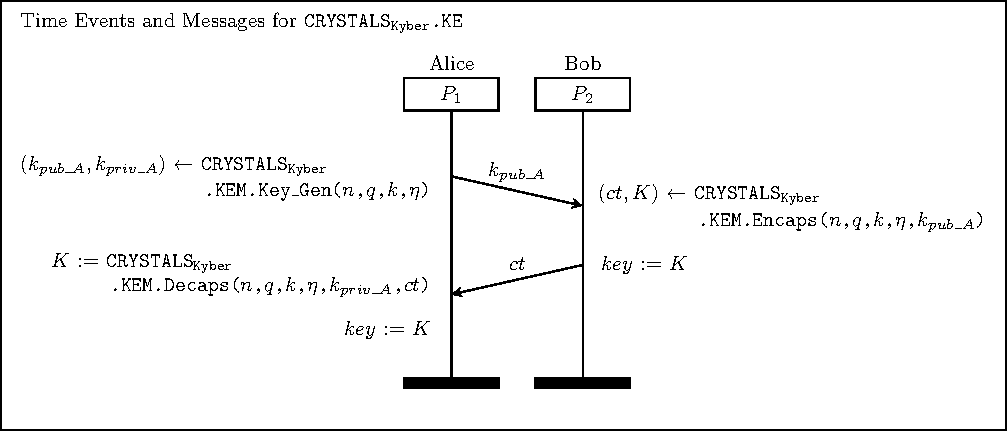
\includegraphics[width=0.8725\textwidth]{figures/sections/section-3/crystals-kyber-key-exchange-protocol-schematic.pdf}
        \caption{Schematic of the CRYSTALS-Kyber Key Exchange protocol,\\ with the respective Time Events and Messages.}
        \label{fig:crystals-kyber-key-exchange-protocol-schematic}
    \end{figure}

    \noindent As mentioned before, we can notice that despite the result of the encapsulation\break \texttt{Encaps} of the \texorpdfstring{\texttt{CRYSTALS}\textsubscript{\texttt{Kyber}}\texttt{.KEM}}\/ algorithm being the pair $(ct, K)$, only the\break ciphertext pair $ct$ is sent to the other party. Then, the other party generates the secret key $K$ by hashing some confidential data decrypted from the ciphertext\break pair $ct$. After the encapsulation and decapsulation procedures, both parties should have the same secret key $K$ at the end of the Key Exchanged Protocol.\break
    
    
    \subsection{CRYSTALS-Dilithium}
    \label{subsec:crystals-dilithium}

    The CRYSTALS-Dilithium \cite{ducas-et-al:crystals-dilithium-algorithm-specifications-and-supporting-documentation:2017:06-2024,ducas-et-al:crystals-dilithium-lattice-based-digital-signature-scheme:2018:06-2024} is a (classical) post-quantum digital signature\break scheme developed to be related and complementary to the CRYSTALS-Kyber asymmetric cryptosystem previously presented, being another component of the CRYSTALS cryptosuite. Therefore, this digital signature scheme is also quantum-resistant and intended to be computationally secure against future cryptanalytic attacks performed by future quantum computers with considerable\break processing power, also ensuring security in the classical contexts. Namely, this cryptographic primitive also uses the computational hardness of the MLWE Problem as its trapdoor function and has most of its security notions based on it. For this reason, this cryptographic digital signature scheme is considered strongly secure under a Chosen-Message Attack (CMA) model. The security\break notion used on this cryptosystem means that an adversary with access to a\break signing oracle cannot produce a signature of a message whose signature it has not yet seen nor produce a different signature of a message it already saw signed.
    
    Moreover, CRYSTALS-Dilithium is one of the first selected standards for digital signatures in the NIST Post-Quantum Cryptography Standardization project, together with FAst-fourier Lattice-based Compact signatures Over Ntru (FALCON) \cite{gentry-peikert-vaikuntanathan:trapdoors-hard-lattices-and-new-cryptographic-constructions:2007:06-2024,fouque-et-al:falcon-fast-fourier-lattice-based-compact-signatures-over-ntru:2019:06-2024} and Stateless Practical Hash-based Incredibly Nice\break Cryptographic Signatures${}^{+}$ (SPHINCS${}^{+}$) \cite{bernstein-et-al:sphincs-practical-stateless-hash-based-signatures:2015:06-2024,bernstein-et-al:sphincs+-signature-framework:2019:06-2024} to replace the current digital signatures that are insecure against to attacks from quantum computers.
    
    
    \vspace{-3ex}
    \begin{figure}[!ht]
        \centering
        \captionsetup{justification=centering}
        
\includegraphics[width=0.6\textwidth]{figures/sections/section-3/crystals-dilithium.pdf}
        \caption{Logotype of CRYSTALS-Dilithium cryptographic primitive.}
        \label{fig:crystals-dilithium-logo}
    \end{figure}


    \noindent The core design of the primitive CRYSTALS-Dilithium is based mainly on a cryptographic technique known as ``Fiat-Shamir with Aborts'', proposed by Vadim Lyubashevsky in 2009 \cite{lyubashevsky:fiat-shamir-with-aborts-applications-lattice-and-factoring-based-signatures:2009:06-2024,lyubashevsky:lattice-signatures-without-trapdoors:2012:06-2024}. This technique uses rejection sampling to make lattice-based Fiat-Shamir digital signatures \cite{fiat-shamir:how-prove-yourself-practical-solutions-identification-and-signature-problems:1987:06-2024} compact and secure.\break It is possible to create digital signature schemes applying this approach, and with small signature sizes, based on the hardness assumption of the mathematical\break problem used in the NTRU lattice-based cryptosystem \cite{hoffstein-pipher-silverman:ntru-ring-based-public-key-cryptosystem:1998:06-2024} that crucially\break uses random samplings from Gaussian probability distributions. However, since it is hard and non-trivial to implement random samplings from the Gaussian probability distribution, the CRYSTALS-Dilithium digital signature scheme uses only the uniform probability distribution to obtain those random samplings.
    
    In particular, this cryptographic primitive improved the previous most\break efficient digital signature scheme known that only uses the uniform probability\break distribution for random samplings, proposed by Shi Bai and Steven Galbraith in 2013 \cite{bai-galbraith:improved-compression-technique-signatures-based-learning-with-errors:2013:06-2024}. Namely, CRYSTALS-Dilithium digital signature scheme uses a new\break technique that shrinks the size of the public key by more than half. This digital\break signature scheme has the smallest public key and signature sizes of any known lattice-based digital signature scheme that only uses a uniform probability\break distribution for the random samplings. However, it may have larger sizes for the signature, public key, and private key when we compare it to the other digital signature schemes NIST also selected as new standards in the NIST\break Post-Quantum Cryptography Standardization project. Namely, it has larger public and private keys than SPHINCS${}^{+}$ hash-based digital signature \cite{bernstein-et-al:sphincs-practical-stateless-hash-based-signatures:2015:06-2024,bernstein-et-al:sphincs+-signature-framework:2019:06-2024}\break in spite of having shorter signatures. Additionally, the FALCON lattice-based\break digital signature \cite{gentry-peikert-vaikuntanathan:trapdoors-hard-lattices-and-new-cryptographic-constructions:2007:06-2024,fouque-et-al:falcon-fast-fourier-lattice-based-compact-signatures-over-ntru:2019:06-2024} has smaller sizes for the signature, public key, and\break private key than the CRYSTALS-Dilithium digital signature scheme. However, the former uses a Gaussian probability distribution for the random samplings.


    \subsubsection{CRYSTALS-Dilithium Digital Signature}
    \label{subsubsec:crystals-dilithium-digital-signature}

    Let $n$, $\ell$, ${\gamma}_{1}$, $\omega$, and $k$ be positive integer parameters, and recall that $n = 256$.\break Additionally, let $\mathcal{M} = { \{ 0 , 1 \} }^{*}$ denote the messages space, where every message\break $m \in \mathcal{M}$ will be cryptographically hashed jointly with a random seed of $256$ bits, outputting a value $\mu$ of $512$ bits to be used then to produce the final signature.\break Now, consider the digital signature scheme denoted by the tuple of cryptographic\break procedures of the form \texorpdfstring{\texttt{CRYSTALS}\textsubscript{\texttt{Dilithium}}\texttt{.Signature} = \big(\texttt{Key\_Gen}, \texttt{Sign}, \texttt{Verify}\big)}\/. Here, the signatures are composed of the vectors $\tilde{c}$, $z$, and $h$, having the form:
    \begin{equation*}
        \begin{split}
            \sigma = (\tilde{c}, z, h)& \in \left( { \{ 0, 1 \} }^{n} \times { \{ 0, 1 \} }^{\left( n \times \ell \times (1 + \log_{2}({\gamma}_{1}) \right) } \times { \{ 0, 1 \} }^{\left( 8 \times ( \omega + k ) \right) } \right) = \\
            & = \left( { \{ 0, 1 \} }^{256} \times { \{ 0, 1 \} }^{\left( 256 \times \ell \times (1 + \log_{2}({\gamma}_{1}) \right) } \times { \{ 0, 1 \} }^{\left( 8 \times ( \omega + k ) \right) } \right)
        \end{split}
    \end{equation*}
    
    \noindent For the currently recommended standards, we have $\ell \in \{4,5,7\}$, ${\gamma}_{1} \in \{ {2}^{17}, {2}^{19} \}$, $\omega \in \{ 55, 75, 80 \}$, and $k \in \{4,6,8\}$. However, other configurations are possible as well, depending on the security level desirable for the digital signature scheme.

    \vspace{1ex}

    \noindent In order to properly define the \texorpdfstring{\texttt{CRYSTALS}\textsubscript{\texttt{Dilithium}}}\/ digital signature scheme\break \texttt{Signature}, we need to formulate the sub-routines \texttt{Key\_Gen}, \texttt{Sign}, and \texttt{Verify}.

    \clearpage
    
    First, we should start by defining the sub-routine \texttt{Key\_Gen} for the generation of the asymmetric key pair composed of a public and a private (secret) key. This sub-routine receives as inputs, the integer parameters $n \in \mathbb{Z}$, $k \in \mathbb{Z}$, $\ell \in \mathbb{Z}$, $q \in \mathbb{Z}$, $\eta \in \mathbb{Z}$, and ${d}_{t} \in \mathbb{Z}$. Namely, the parameter $n$ determines the dimension of the polynomial ring $\mathcal{R}$, the parameter $k$ determines the number of polynomials in the module being used, $\ell$ determines the number of secret polynomials, $q$ defines the modulo for the polynomial coefficients, and the parameter $\eta$ is related to the\break (random) noise distributions, determining as well the secret key range. The\break parameters $k$, $\ell$, and $\eta$ are related to the security of the asymmetric keys\break generated. The first two can tune up the complexity of the MLWE Problem, while the latter is critical for security by adding randomness to the sub-routine.

    \vspace{2ex}

    \noindent The pseudo-code of the sub-routine \texttt{Key\_Gen} of the \texorpdfstring{\texttt{CRYSTALS}\textsubscript{\texttt{Dilithium}}}\/ asymmetric digital signature scheme algorithm \texttt{Signature} is defined as we present below:
    \vspace{-3.75ex}
    \begin{algorithm}
        \caption{\texorpdfstring{\texttt{CRYSTALS}\textsubscript{\texttt{Dilithium}}\texttt{.Signature}\\ \phantom{......................................................}\texttt{.Key\_Gen}($n$, $k$, $\ell$, $q$, $\eta$, ${d}_{t}$)}\/: Key Generation}
        \label{subrou:crystals-dilithium-key-gen}
        
        \textbf{Input:} $\left( n, k, \ell, q, \eta, {d}_{t} \right)$\\
        \textbf{Output:} $ ( {k}_{pub}, {k}_{priv} ) $
    
        \begin{algorithmic}[1]
            \Require $n = 256$, $q = 8380417$, ${d}_{t} = 13$, $k > 0$, $\ell > 0$, $\eta > 0$
            \Ensure $n \in \mathbb{Z},\ k \in \mathbb{Z},\ \ell \in \mathbb{Z},\ q \in \mathbb{Z},\ \eta \in \mathbb{Z},\ {d}_{t} \in \mathbb{Z}$
            
            \vspace{2ex}
            
            \State $\zeta \gets { \{ 0 , 1 \} }^{n} = { \{ 0 , 1 \} }^{256}$
            \State $(\rho, \rho', K) \sim \left(\ { \{ 0 , 1 \} }^{n} \times { \{ 0 , 1 \} }^{ (2 \times n) } \times { \{ 0 , 1 \} }^{n}\ \right) = $
            \Statex \hspace{15ex} $ = \left(\ { \{ 0 , 1 \} }^{256} \times { \{ 0 , 1 \} }^{512} \times { \{ 0 , 1 \} }^{256}\ \right)$ := $H( \zeta )$
            \State $A \sim {\mathcal{R}}_{q}^{( k \times \ell )} = {\mathcal{R}}_{8380417}^{( k \times \ell )}$ := \texttt{Sample}($\rho$)
            \State $(s, e) \sim \left( {\Upsilon}_{\eta}^{\ell} \times {\Upsilon}_{\eta}^{k} \right)$ := \texttt{Sample}($\rho'$)
            \State $t$ := $A \times s + e$
            \State $({t}_{1}, {t}_{0})$ := \texttt{Compress}\textsubscript{$q$}$\left( t, {d}_{t} \right)$ = \texttt{Power2Round}\textsubscript{$q$}$\left( t, {d}_{t} \right)$
            \State ${t}_{r} \sim { \{ 0 , 1 \} }^{n} = { \{ 0 , 1 \} }^{256}$ := $H\left( \rho\ ||\ {t}_{1} \right)$
            
            \vspace{1ex}
            
            \State ${k}_{pub}$ := $\left( \rho, {t}_{1} \right)$
            \State ${k}_{priv}$ := $\left( \rho, K, {t}_{r}, s, e, {t}_{0} \right)$
            
            \vspace{1ex}
            
            \State \Return $( {k}_{pub}, {k}_{priv} )$
        \end{algorithmic}
   
    \end{algorithm}
    \vspace{-3.75ex}

    \noindent The resulting output of the sub-routine \texttt{Key\_Gen} of the \texorpdfstring{\texttt{CRYSTALS}\textsubscript{\texttt{Dilithium}}}\/ digital signature scheme algorithm \texttt{Signature} is an asymmetric key pair composed by the public key ${k}_{pub}$ and the private key ${k}_{priv}$. The public key ${k}_{pub}$ is a pair composed of the random (or pseudo-random) seed $\rho$ and the public target vector ${t}_{1}$, while the private key ${k}_{priv}$ is composed of the random (or pseudo-random) seed $\rho$, the (random) secret seed key $K$, the random (coin) target vector ${t}_{r}$, the secret vector $s$, the error (noise) vector $e$, and the low-order bit target vector ${t}_{0}$. The random seed $\rho$ is usually a $256$-bit string used to send a Pseudo-Random Function (PRF) or cryptographic hash function, from which the coefficients of the polynomials in the matrix $A$ are generated. The random seed $\rho'$ is usually a $512$-bit string used to generate the random secret vector $s$ and the error (noise) vector. Furthermore, the public target vector $t$ is compressed by a parameter ${d}_{t}$ defined \textit{a priori} that refers to the number of bits dropped from that vector on the compression of the encoded information during the key generation procedure.

    \vspace{1ex}
    
    Now we can define the sub-routine \texttt{Sign} for the creation of a digital signature\break on some given message. Namely, this sub-routine receives as inputs, the integer\break parameters $n \in \mathbb{Z}$, $k \in \mathbb{Z}$, $\ell \in \mathbb{Z}$, $q \in \mathbb{Z}$,  ${\gamma}_{1} \in \mathbb{Z}$, ${\gamma}_{2} \in \mathbb{Z}$, $\tau \in \mathbb{Z}$, $\eta \in \mathbb{Z}$, $m \in \mathcal{M} = { \{0, 1\} }^{*}$. The input $m$ is the message to be signed, while ${k}_{priv}$ is the private key generated by the party signing the message $m$, guaranteeing the\break authenticity of the same. Once again, the parameter $n$ determines the dimension of the polynomial ring $\mathcal{R}$, the parameter $k$ determines the number of polynomials in the module being used, $\ell$ determines the number of secret polynomials, and $q$ defines the modulo for the polynomial coefficients. The parameter ${\gamma}_{1}$ is the\break coefficient range for a (random) mask vector $y$, related to the (random) noise distributions used for maskings required to generate randomness and uniqueness for each signature produced. This (random) mask vector $y$ is crucial to create a commitment vector $w$, which will be used to generate a challenge vector $c$. The (random) mask vector $y$ and the challenge vector $c$, jointly with the secret vector $s$ from the private key ${k}_{priv}$, will be used to create a response target vector $z$,\break following the mathematical structure of the MLWE Problem. The parameter ${\gamma}_{2}$ sets a low-order rounding range bound on the polynomial coefficients of the\break commitment vector $w$ to ensure those coefficients are not too large. The\break parameter $\tau$ determines the number of non-zero values (i.e., $\pm 1$ values) on the challenge vector $c$. Similar to the previously described key generation procedure, the input parameters $k$, $\ell$, ${\gamma}_{1}$, and ${\gamma}_{2}$ are related to the security of the digital signatures produced. The first two can tune up the complexity of the MLWE Problem, while the remaining ones are critical for efficiency and performance by being closely related to the rate of rejection of the potential signature candidates.

    \vspace{1ex}
    
    \noindent The resulting output of the sub-routine \texttt{Sign} of the \texorpdfstring{\texttt{CRYSTALS}\textsubscript{\texttt{Dilithium}}}\/ digital signature scheme algorithm \texttt{Signature} is a digital signature $\sigma$ composed by the (compressed) challenge vector $\tilde{c}$, the response target vector $z$, and the hint vector $h$. The (compressed) challenge vector $\tilde{c}$ aims to improve the efficiency of the signature $\sigma$ in terms of its size and transmission. From the (compressed) challenge vector $\tilde{c}$, the party verifying the signature $\sigma$ will be able to sample and uncompress it to the (real) challenge vector $c$. The response target vector $z$ is the response related to the challenge vector $c$ following the mathematical structure of an MLWE Problem. Then, the hint vector $h$ aims to help the other party recover certain polynomial coefficients of the commitment derived from the signature, thus validating the authenticity and integrity of the signed message. This hint vector ensures that the signature $\sigma$ is valid without needing to store or transmit large amounts of data. The random seed $\rho$ is usually a $256$-bit string used to generate the coefficients of the polynomials in the matrix $A$. The random seed $\rho'$ is usually a $512$-bit string used to generate the (random) mask vector $y$ required to create the commitment vector $w$ and the response target vector $z$.

    \vspace{1ex}

    \noindent The pseudo-code of the sub-routine \texttt{Sign} of the \texorpdfstring{\texttt{CRYSTALS}\textsubscript{\texttt{Dilithium}}}\/ asymmetric digital signature scheme \texttt{Signature} is defined as we present in sub-routine \ref{subrou:crystals-dilithium-sign}.
    
    \clearpage

    \begin{algorithm}
        \caption{\texorpdfstring{\texttt{CRYSTALS}\textsubscript{\texttt{Dilithium}}\\ \phantom{............................}\texttt{.Signature}\texttt{.Sign}($n, k, \ell, q, {\gamma}_{1}, {\gamma}_{2}, \tau, \eta, \omega,\\ \phantom{..........................................................}{k}_{priv} = (\rho, K, {t}_{r}, s, e, {t}_{0}), m$)}\/:\\ \phantom{...........................................................................................}Message Signing}
        \label{subrou:crystals-dilithium-sign}
        
        \textbf{Input:} $\left( n, k, \ell, q, {\gamma}_{1}, {\gamma}_{2}, \tau, \eta, \omega, {k}_{priv}, m \right)$\\
        \textbf{Output:} $ \sigma $
    
        \begin{algorithmic}[1]
            \Require $n = 256$, $q = 8380417$, $k > 0$, $\ell > 0$, ${\gamma}_{1} > 0$, ${\gamma}_{2} > 0$, $\tau > 0$, $\eta > 0$, $\omega > 0$
            \Ensure \begin{varwidth}[t]{\linewidth}$n \in \mathbb{Z},\ k \in \mathbb{Z},\ \ell \in \mathbb{Z},\ q \in \mathbb{Z},\ {\gamma}_{1} \in \mathbb{Z},\ {\gamma}_{2} \in \mathbb{Z},\ \tau \in \mathbb{Z},$ \par $ \eta \in \mathbb{Z},\ \omega \in \mathbb{Z},\ m \in \mathcal{M} = {\{0, 1\}}^{*}$ \end{varwidth}
            
            \vspace{2ex}

            \State $\left( \rho, K, {t}_{r}, s, e, {t}_{0} \right) \gets {k}_{priv}$
            
            \vspace{1ex}
            
            \State $A \sim {\mathcal{R}}_{q}^{( k \times \ell )} = {\mathcal{R}}_{8380417}^{( k \times \ell )}$ := \texttt{Sample}($\rho$)
            \State $\mu \sim { \{ 0 , 1 \} }^{( 2 \times n )} = { \{ 0 , 1 \} }^{512}$ := $H\left( {t}_{r}\ ||\ m \right)$
            \State $\kappa$ := $0$
            \State $(z, h)$ := $\bot$
            \State $\rho' \sim { \{ 0 , 1 \} }^{( 2 \times n )} = { \{ 0 , 1 \} }^{512}$ := $H\left( K\ ||\ \mu \right)$ (or $\sigma \gets { \{ 0 , 1 \} }^{( 2 \times n )} = { \{ 0 , 1 \} }^{512}$ 
            \Statex \hspace{44ex} for randomized signing)
            
            \vspace{1ex}

            \While{$(z, h) = \bot$}
                \State $y \sim { \tilde{\Upsilon} }_{ { \gamma }_{1} }^{\ell}$ := \texttt{SampleMask}$( \rho', \kappa )$
                \State $w$ := $A \times y$
                \State ${w}_{1}$ := \texttt{HighBits}\textsubscript{$q$}$( w, 2 \times {\gamma}_{2} )$
                \State $\tilde{c} \sim { \{ 0 , 1 \} }^{n} = { \{ 0 , 1 \} }^{256}$ := $H\left( \mu\ ||\ {w}_{1} \right)$
                \State $c \sim {B}_{\tau}$ := \texttt{SampleInBall}${}_{\tau}$$(\tilde{c})$
                \State $z$ := $y + c \times s$
                \State ${r}_{0}$ := \texttt{LowBits}\textsubscript{$q$}$( w - c \times e, 2 \times {\gamma}_{2} )$
                \State $\beta$ := $\tau \times \eta$
                
                \vspace{1ex}

                \If{ $ \left(\ \left\llbracket\ {\big|\big| z \big|\big|}_{\infty} \geq {\gamma}_{1} - \beta\ \right\rrbracket\ \mathrm{or}\ \left\llbracket\ { \big|\big|{r}_{0} \big|\big| }_{\infty} \geq {\gamma}_{2} - \beta \ \right\rrbracket\ \right) $ }
                    \State $(z, h)$ := $\bot$ 
                \Else
                    \State $h$ := \texttt{MakeHint}\textsubscript{$q$}$( -c \times {t}_{0}, w - c \times e + c \times {t}_{0}, 2 \times {\gamma}_{2} )$
                    \If{ $ \left(\ \left\llbracket\ { \big|\big| c \times {t}_{0} \big|\big| }_{\infty} \geq {\gamma}_{2} \ \right\rrbracket\ \mathrm{or}\ \left\llbracket\ weight(h) > \omega \ \right\rrbracket\ \right) $ }
                        \State $(z, h)$ := $\bot$ 
                    \EndIf
                \EndIf

                \vspace{1ex}

                \State $\kappa$ := $\kappa + \ell$

                \vspace{1ex}
                
            \EndWhile
            
            \vspace{1ex}
            
            \State $\sigma = \left( \tilde{c}, z, h \right)$
            
            \vspace{1ex}
            
            \State \Return $\sigma$
        \end{algorithmic}
   
    \end{algorithm}
    
    \vfill
    
    \clearpage
    
    Then, we can define the sub-routine \texttt{Verify} for the verification of a digital\break signature on some given message. This sub-routine receives as inputs, the integer\break parameters $n \in \mathbb{Z}$, $k \in \mathbb{Z}$, $\ell \in \mathbb{Z}$, $q \in \mathbb{Z}$, ${d}_{t} \in \mathbb{Z}$, ${\gamma}_{1} \in \mathbb{Z}$, ${\gamma}_{2} \in \mathbb{Z}$, $\tau \in \mathbb{Z}$, $\eta \in \mathbb{Z}$, $\omega \in \mathbb{Z}$, $m \in \mathcal{M} = { \{0, 1\} }^{*}$. The input $m$ is the message supposedly related to the\break digital signature $\sigma$, while ${k}_{pub}$ is the public key generated by the party verifying the digital signature $\sigma$. Once again, the parameter $n$ determines the dimension of the polynomial ring $\mathcal{R}$, the parameter $k$ determines the number of polynomials\break in the module being used, $\ell$ determines the number of secret polynomials, and $q$ defines the modulo for the polynomial coefficients. The parameter ${\gamma}_{1}$ is the\break coefficient range for the response vector $z$, setting an upper bound on its\break polynomial coefficients. The parameter ${\gamma}_{2}$ sets a low-order rounding range bound on the polynomial coefficients of the commitment vector $w$ to ensure those\break coefficients are not too large. The parameter $\tau$ determines the number of non-zero\break values (i.e., $\pm 1$ values) on the challenge vector $c$. The parameter $\omega$ sets an upper bound to the Hamming weight of the hint vector $h$. Similar to the previously described key generation procedure, the input parameters $k$, $\ell$, ${\gamma}_{1}$, and ${\gamma}_{2}$ are related to the security of the digital signatures verified. The first two can tune up the complexity of the MLWE Problem, while the remaining ones are critical for the efficiency and performance of the sub-routine by being closely related to the rate of success/failure of the verification procedure applied to a signature.
    
    \vspace{2ex}

    \noindent The pseudo-code of the sub-routine \texttt{Verify} of the \texorpdfstring{\texttt{CRYSTALS}\textsubscript{\texttt{Dilithium}}}\/ asymmetric digital signature scheme algorithm \texttt{Signature} is defined as we present below:
    \vspace{-3.75ex}
    \begin{algorithm}
        \caption{\texorpdfstring{\texttt{CRYSTALS}\textsubscript{\texttt{Dilithium}}\\ \phantom{............................}\texttt{.Signature}\texttt{.Verify}($n, k, \ell, q, {d}_{t}, {\gamma}_{1}, {\gamma}_{2}, \tau, \eta, \omega,\\ \phantom{..............................................................}{k}_{pub} = (\rho, {t}_{1}), m, \sigma=(\tilde{c},z,h)$)}\/:\\ \phantom{....................................................................................}Signature Verification}
        \label{subrou:crystals-dilithium-verify}
        
        \textbf{Input:} $\left( n, k, \ell, q, {d}_{t}, {\gamma}_{1}, {\gamma}_{2}, \tau, \eta, \omega, {k}_{pub}, m, \sigma \right)$\\
        \textbf{Output:} $ is\_valid $
    
        \begin{algorithmic}[1]
            \Require \begin{varwidth}[t]{\linewidth}$n = 256$, $q = 8380417$, ${d}_{t} = 13$, $k > 0$, $\ell > 0$, ${\gamma}_{1} > 0$, ${\gamma}_{2} > 0$,\par $\tau > 0$, $\eta > 0$, $\omega > 0$ \end{varwidth}
            \Ensure \begin{varwidth}[t]{\linewidth}$n \in \mathbb{Z},\ k \in \mathbb{Z},\ \ell \in \mathbb{Z},\ q \in \mathbb{Z},\ {d}_{t} \in \mathbb{Z},\ {\gamma}_{1} \in \mathbb{Z},\ {\gamma}_{2} \in \mathbb{Z},$\par $\tau \in \mathbb{Z},\ \eta \in \mathbb{Z},\ \omega \in \mathbb{Z},\ m \in \mathcal{M} = {\{0, 1\}}^{*}$ \end{varwidth}
            
            \vspace{2ex}

            \State $\left( \rho, {t}_{1} \right) \gets {k}_{pub}$
            
            \vspace{1ex}
            
            \State $A \sim {\mathcal{R}}_{q}^{( k \times \ell )} = {\mathcal{R}}_{8380417}^{( k \times \ell )}$ := \texttt{Sample}($\rho$)
            \State $\mu \sim { \{ 0 , 1 \} }^{( 2 \times n )} = { \{ 0 , 1 \} }^{512}$ := $H\left( H( \rho\ ||\ {t}_{1} )\ ||\ m \right)$
            \State $c$ := \texttt{SampleInBall}${}_{\tau}$($\tilde{c}$)
            \State ${w}_{1}'$ := \texttt{UseHint}\textsubscript{$q$}$( h, A \times z - c \times {t}_{1} \times {2}^{{d}_{t}}, 2 \times {\gamma}_{2} )$
            \State $\beta$ := $\tau \times \eta$

            \vspace{1ex}
            
            \State $is\_valid$ := $\left(\ \big\llbracket\ {\big|\big| z \big|\big|}_{\infty} < {\gamma}_{1} - \beta\ \big\rrbracket\ \mathrm{and}\ \big\llbracket\ \tilde{c} = H(\mu\ ||\ {w}_{1}')\ \big\rrbracket\ \mathrm{and}\ \big\llbracket\ weight(h) \leq \omega\ \big\rrbracket\ \right)$
           
            \vspace{1ex}
            
            \State \Return $is\_valid$
        \end{algorithmic}
   
    \end{algorithm}
    \vspace{-3.75ex}

    \noindent The resulting output of the sub-routine \texttt{Verify} of the \texorpdfstring{\texttt{CRYSTALS}\textsubscript{\texttt{Dilithium}}}\/ digital\break signature scheme algorithm \texttt{Signature} is a \textit{boolean} conjunction $is\_valid$ of three terms. This sub-routine receives the message $m$, as well as the (supposedly)\break related digital signature $\sigma$ composed by the (compressed) challenge vector $\tilde{c}$, the response target vector $z$, and the hint vector $h$. Additionally, the public key ${k}_{pub}$ is also required for this procedure, since its (extracted) components $\rho$ and ${t}_{1}$ will be crucial in several steps. The random seed $\rho$ is usually a $256$-bit string used to generate the coefficients of the polynomials in the matrix $A$. The random seed $\rho$ is also concatenated with the (compressed) target vector ${t}_{1}$ to produce a digest result from the cryptographic hash function $H(\rho\ ||\ {t}_{1})$. The result of this digest is then concatenated with the message $m$, being applied another cryptographic hash function on this concatenation, i.e., $H\left(H( \rho\ ||\ {t}_{1} )\ ||\ m \right)$, to produce a binary\break random string $\mu$ with $512$ bits. From the (compressed) challenge vector $\tilde{c}$, the party verifying the signature $\sigma$ will be able to sample and uncompress it to the (real) challenge vector $c$. Then, using the hint vector $h$ and applying algebraic\break operations involving the lattice matrix $A$, the response target vector $z$, the\break (uncompressed) challenge vector $c$, and the (compressed) target vector ${t}_{1}$, it is computed a commitment vector ${w}_{1}'$. The algebraic operations related to the computation of the commitment vector ${w}_{1}'$ follow the mathematical structure of an MLWE Problem. Finally, the \textit{boolean} conjunction value $is\_valid$ is computed verifying if all these three following \textit{boolean} conditions hold \textit{simultaneously}:
    \begin{enumerate}
        \item The polynomial coefficients of the response vector $z$ are not greater than the upper bound given by ${\gamma}_{1} - \beta$, where $\beta$ is computed as $\beta = \tau \times \eta$;
        \item The digest result of the cryptographic hash function $H(\mu\ ||\ {w}_{1}')$ is equal to the (compressed) challenge vector $\tilde{c}$ extracted from the signature $\sigma$;
        \item The Hamming weight (i.e., the number of bits equal to $1$) of the hint vector $h$ extracted from the signature $\sigma$ is not greater than the upper bound $\omega$.
    \end{enumerate}

    \noindent If the three \textit{boolean} conditions hold, the verification of the given digital signature $\sigma$ related to the given message $m$ succeeded and the signature $\sigma$ is valid.

    The CRYSTALS-Dilithium digital signature uses a pseudo-randomness in the signing procedure generated using the well-known cryptographic hash function Secure Hash Algorithm and KECCAK - 256 (SHAKE-256)\footnote{The cryptographic hash function SHAKE-256$(M,d)$, differently from the well-known cryptographic hash function SHA-256, can have an output of arbitrary size.} from the Secure Hash Algorithm - 3 (SHA-3) family as a deterministic function of the message to be signed and a small secret key (see the steps 3 and 6 of the sub-routine \ref{subrou:crystals-dilithium-sign}). Since most of the signing procedure may need to be repeated several times in a computational loop until we build a final signature, a counter $\kappa$ is also appended during the creation of the (random) mask vector $y$, which will be the input of the SHAKE-256 cryptographic hash function making its output differs with each signing attempt of the same message $m$. Because each (possibly long) message $m$ may require several iterations to be successfully signed, we compute an initial\break hash digest of the (initial) message $m$ using a collision-resistant cryptographic\break hash function (see the step 3 of the sub-routine \ref{subrou:crystals-dilithium-sign}). Then, we use the respective hash digest as the input of the cryptographic hash function in the computational loop throughout the signing procedure (see steps 3 and 11 of the sub-routine \ref{subrou:crystals-dilithium-sign}).

    Additionally, one of the primary implementation design improvements offered\break by the CRYSTALS-Dilithium digital signature scheme over the previous ones is the fact that the size of the public key is approximately halved, at the\break expense of little longer signatures with fewer than a hundred extra bytes. In order to perform this size reduction, the key generation sub-routine outputs\break ${t}_{1}$ := \texttt{Power2Round}\textsubscript{$q$}$\left( t, {d}_{t} \right)$ as a part of the public key, dropping at average ${d}_{t}$ bits per polynomial coefficient. Then, the public key requires $\lceil \log{(q)} \rceil - {d}_{t}$ bits per\break coefficient of the ring polynomial. In the configurations proposed by the authors,\break we assume $q \approx {2}^{23} = 8388608$ and ${d}_{t} = 13$, which means that instead of 23 bits in each coefficient of the public key, there is instead only 10 bits (i.e., $\lceil \log{(q)} \rceil - {d}_{t} = \lceil \log{ ({2}^{23}) } \rceil - 13 = 23 - 13 = 10$), what results in a compression of the size of the public key generated (see the step 6 of the sub-routine \ref{subrou:crystals-dilithium-key-gen}).

    The main complication of not having the entire target vector $t$ in the public key ${k}_{pub}$ is that it is no longer possible to compute exactly the commitment vector ${w}_{1}'$ in the signature verification sub-routine. The signature verification will need the high-order bits of the result of the algebraic operation $A \times z - c \times t$ to compute this, but it can only compute $A \times z - c \times {t}_{1} \times {2}^{{d}_{t}} = A \times z - c \times t + c \times {t}_{0}$  (see the step 5 of the sub-routine \ref{subrou:crystals-dilithium-verify}). Even though the high-order bits of $c \times {t}_{0}$ are $0$, its presence in the sum creates ``carry'' bits which may affect the higher bits. The signer of the message thus sends these ``carries'' as a hint vector $h$ to the verifier of the signature. Heuristically, based on the parameter choices proposed by the authors, there should not be more than $\omega$ positions in which a ``carry'' is caused. Therefore, the signer of the message simply sends the positions in which these ``carries'' occur, which allows the verifier to compute the high order bits of $A \times z - c \times t$ with the support given by the hint vector $h$ (these are the extra bytes in CRYSTALS-Dilithium compared to other previous digital signatures).

    In order to keep the size of the public and private keys small, both the \texttt{Sign} and \texttt{Verify} procedures begin with extracting the matrix $A$, or more accurately,\break its Number-Theoretic Transform (NTT) \cite{agarwal-burrus:number-theoretic-transforms-implement-fast-digital-convolution:1975:06-2024} domain representation $\hat{A}$ from the\break (public) pseudo-random seed $\rho$. If storage space is not a factor, then the NTT\break domain representation matrix $\hat{A}$ can be pre-computed and be part of both the public and private keys. The signer of the message $m$ can additionally\break pre-compute the NTT domain representations of the secret vector $s$, error (noise) vector $e$, and target vector ${t}_{0}$ to slightly speed up the signing sub-routine. On the other hand, if the signer of the message $m$ wants to store a private key as small as possible, it only needs to store a secret seed $\zeta$ with $256$ bits, which is used to generate the pseudo-randomness to create the pseudo-random seed $\rho$, the secret key $K$, the secret vector $s$, and the error (noise) vector $e$, in the key generation\break sub-routine. Furthermore, we can keep the memory usage low for some of the\break intermediate computations required by only keeping the parts of the NTT\break domain representation we are currently working on within all the procedures. For more details about this implementation with low memory usage, see the original proposal of the CRYSTALS-Dilithium digital signature scheme.

    We can use the CRYSTALS-Dilithium cryptographic primitive to produce deterministic or randomized digital signatures. The former always gives the same digital signature output $\sigma$ for a given message $m$ since we derive the random seed $\rho'$ from the hashed message $\mu$ and a secret key $K$. The latter does not produce the same digital signature output $\sigma$ for a particular message since we choose the random seed $\rho'$ completely at random (see step 6 of the sub-routine \ref{subrou:crystals-dilithium-sign}).
    
    In situations where some side channels that exploit determinism are possible\break \cite{samwel-et-al:breaking-ed25519-wolfssl:2018:06-2024,poddebniak-et-al:attacking-deterministic-signature-scheme-using-fault-attacks:2018:06-2024}, we may use the randomized variant of this digital signature scheme. Another case where we may want to avoid determinism is when the signer party does not wish to reveal the content of the message $m$ the sender party is signing. When the digital signature scheme is deterministic, despite not occurring timing leakage of the secret key $K$, there is a timing leakage of the hashed message $\mu$. For this case, and since we derive the randomness of this signature from the value $\mu$, the number of aborts for a particular message will always be the same.

    \vspace{1ex}

    \noindent After defining the key generation, signing, and verification procedures, we need to show this digital signature scheme is correct (or sound) and capable of signing\break messages and verifying digital signatures correctly (i.e., with a negligible failure\break probability). However, to prove the correctness of this digital signature, we need to define a set of lemmas that highlight the properties of the algorithms \texttt{MakeHint}${}_{q}$, \texttt{UseHint}${}_{q}$, \texttt{Decompose}${}_{q}$, \texttt{HighBits}${}_{q}$, and \texttt{LowBits}${}_{q}$ \cite{ducas-et-al:crystals-dilithium-algorithm-specifications-and-supporting-documentation:2017:06-2024,ducas-et-al:crystals-dilithium-lattice-based-digital-signature-scheme:2018:06-2024}.

    \paragraph{\textbf{Lemma 1:}} Suppose that $q$ and $\alpha$ are positive integer numbers, where $q > 2 \times \alpha$, $q \equiv 1$ (mod $\alpha$), and $\alpha$ is an even number. Let $r$ and $z$ be vectors containing elements in ${\mathcal{R}}_{q}$ where ${||z||}_{\infty} \leq \frac{\alpha}{2}$, and let $h$, $h'$ be binary hint values. Then, the \texttt{HighBits}${}_{q}$, \texttt{MakeHint}${}_{q}$, and \texttt{UseHint}${}_{q}$ algorithms satisfy the following properties: 
    \begin{enumerate}
        \item \texttt{UseHint}${}_{q}$(\texttt{MakeHint}${}_{q}$($z$, $r$, $\alpha$), $r$, $\alpha$) = \texttt{HighBits}${}_{q}$($r + z$, $\alpha$);
        \item Let ${v}_{1}$ = \texttt{UseHint}${}_{q}$($h$, $r$, $\alpha$). Then, we also verify that ${||r - {v}_{1} \times \alpha||}_{\infty} \leq \alpha + 1$. Furthermore, if the Hamming weight of the vector $h$ is equal to $\omega$, then all except at most $w$ coefficients of the result $r - {v}_{1} \times \alpha$ will have magnitude at most $\frac{\alpha}{2}$ after centered reduction modulo $q$ using modular multiplications;
        \item For any values $h$ and $h'$, if we verify \texttt{UseHint}${}_{q}$($h, r, \alpha$) = \texttt{UseHint}${}_{q}$($h', r, \alpha$), then we can conclude those binary hint values $h$ and $h'$ are equal.
    \end{enumerate}

    \paragraph{\textbf{Lemma 2:}} If we verify that ${||s||}_{\infty} \leq \beta$ and ${||\mathrm{\texttt{LowBits}}{}_{q}(r, \alpha)||}_{\infty} < \frac{\alpha}{2} - \beta$, where $s$ is the secret vector on the MLWE Problem formulation and $\beta = \tau \times \eta$. Then, we can also verify that the equality \texttt{HighBits}${}_{q}$($r, \alpha$) = \texttt{HighBits}${}_{q}$($r + s, \alpha$) holds.

    \paragraph{\textbf{Lemma 3:}} Let $({r}_{1}, {r}_{0})$ = \texttt{Decompose}${}_{q}$($r, \alpha$), $({w}_{1}, {w}_{0})$ = \texttt{Decompose}${}_{q}$($r + s, \alpha$), and ${||s||}_{\infty} \leq \beta$, where $s$ is the secret vector on the MLWE Problem formulation and $\beta = \tau \times \eta$. Then, ${||s + {r}_{0}||}_{\infty} < \frac{\alpha}{2} - \beta \Longleftrightarrow {w}_{1} = {r}_{1} \wedge {||{w}_{0}||}_{\infty} < \frac{\alpha}{2} - \beta$ holds.

    \paragraph{\textbf{Lemma 4:}} Let $q \in \mathbb{Z}$, $\alpha \in \mathbb{Z}$, $r \in {\mathbb{Z}}_{q}$, and $z \in {\mathbb{Z}}_{q}$, with ${||z||}_{\infty} \leq \frac{\alpha}{2}$. Then, we verify the equality \texttt{UseHint}${}_{q}$(\texttt{MakeHint}${}_{q}$($z, r, \alpha$), $r, \alpha$) $=$ \texttt{HighBits}${}_{q}$($r + z, \alpha$).

    \paragraph{\textbf{Lemma 5:}} Let $(h,r) \in \{ 0, 1 \} \times {\mathbb{Z}}_{q}$ and let ${v}_{1} = $\texttt{UseHint}${}_{q}$($h, r, \alpha$). If $h = 0$ holds, then we verify ${|| r - {v}_{1} \times \alpha ||}_{\infty} \leq \frac{\alpha}{2}$, else we verify ${|| r - {v}_{1} \times \alpha ||}_{\infty} \leq \alpha + 1$.

    \paragraph{\textbf{Lemma 6:}} Let $q \in \mathbb{Z}$, $\alpha \in \mathbb{Z}$, $r \in {\mathbb{Z}}_{q}$, $h \in \{ 0, 1 \}$, and $h' \in \{ 0, 1 \}$. If the equality \texttt{UseHint}${}_{q}$($h, r, \alpha$) $=$ \texttt{UseHint}${}_{q}$($h', r, \alpha$) holds, then the equality $h = h'$ also holds.

    \vspace{2.5ex}
    
    \noindent Now, we need to derive the proofs of the first three lemmas, where the last three lemmas serve as auxiliary lemmas for the proof of each one of the three properties of the first lemma. The respective lemma proofs are shown below:

    \paragraph{\textbf{Proof of Lemma 1:}}\mbox{\\}
    
    \paragraph{$\bullet$ \textbf{Proof of Property 1 using Lemma 4:}} The output of the algorithm \texttt{Decompose}${}_{q}$ are given by two integer numbers ${r}_{0}$ and ${r}_{1}$, such that $0 \leq {r}_{1} < \frac{(q - 1)}{\alpha}$ and ${|| {r}_{0} ||}_{\infty} \leq \frac{\alpha}{2}$. Due to ${|| z ||}_{\infty} \leq \frac{\alpha}{2}$, the integer number ${v}_{1}$ := \texttt{HighBits}${}_{q}$($r + z, \alpha$) either stays with the same value as ${r}_{1}$ or becomes equal to ${r}_{1} \pm 1$ modulo $m = \frac{(q - 1)}{\alpha}$. More precisely, if ${r}_{0} > 0$, then $-\frac{\alpha}{2} < {r}_{0} + z \leq \alpha$, which implies that ${v}_{1} = {r}_{1}$ or ${v}_{1} = {r}_{1} + 1\ \text{mod}\ m$. If ${r}_{0} \leq 0$, then $-\alpha \leq {r}_{0} + z \leq \frac{\alpha}{2}$, which implies that ${v}_{1} = {r}_{1}$ or ${v}_{1} = {r}_{1} - 1\ \text{mod}\ m$. The algorithm \texttt{MakeHint}${}_{q}$ checks whether ${r}_{1} = {v}_{1}$ and outputs the value $0$ in that case, and outputs the value $1$ when ${r}_{1} \neq {v}_{1}$. The algorithm \texttt{UseHint}${}_{q}$ uses the hint vector $h$ to either output the single value ${r}_{1}$ when we verify $y = 0$ or, depending on whether ${r}_{0} > 0$ holds or not, output either the value ${r}_{1} + 1\ \text{mod}{}^{+}\ m$ or the value ${r}_{1} - 1\ \text{mod}{}^{+}\ m$.
    
    \paragraph{$\bullet$ \textbf{Proof of Property 2 using Lemma 5:}} The \textit{Lemma 5} shows that the value $r$ is not too far away from the output value of the algorithm \texttt{UseHint}${}_{q}$ algorithm. This lemma is necessary for the security of the digital signature scheme. Namely, let $({r}_{1}, {r}_{0})$ := \texttt{Decompose}${}_{q}$($r, \alpha$). Then, for each of three possible cases of outputs of the algorithm \texttt{UseHint}${}_{q}$, we have the following enumerated set of results:
    \begin{enumerate}
        \item If we verify $h = 0$, we have the equality ${v}_{1} = {r}_{1}$ and the equality given by $r - {v}_{1} \times \alpha = {r}_{1} \times \alpha + {r}_{0} - {r}_{1} \times \alpha = {r}_{0}$ with an absolute value at most $\frac{\alpha}{2}$;
        \item If we verify $h = 1$ and ${r}_{0} > 0$, we have the equality ${v}_{1} = {r}_{1} + 1 - \kappa \times \frac{(q - 1)}{\alpha}$ for $\kappa = 0$ or $\kappa = 1$. Therefore, we have the following mathematical equalities:
        \begin{equation*}
            \begin{split}
                r - {v}_{1} \times \alpha & = {r}_{1} \times \alpha + {r}_{0} - \left({r}_{1} + 1 - \kappa \times \frac{(q - 1)}{\alpha} \right) \times \alpha \\
                & = -\alpha + {r}_{0} + \kappa \times (q - 1)
            \end{split}
        \end{equation*}        
        After performing a centered reduction modulo $q$, the latter mathematical expression $-\alpha + {r}_{0} + \kappa \times (q - 1)$ has a magnitude value lower or equal to $\alpha$;
        \item If we verify $h = 1$ and ${r}_{0} \leq 0$, we have the equality ${v}_{1} = {r}_{1} - 1 + \kappa \times \frac{(q - 1)}{\alpha}$ for $\kappa = 0$ or $\kappa = 1$. Therefore, we have the following mathematical equalities:
        \begin{equation*}
            \begin{split}
                r - {v}_{1} \times \alpha & = {r}_{1} \times \alpha + {r}_{0} - \left({r}_{1} - 1 + \kappa \times \frac{(q - 1)}{\alpha} \right) \times \alpha \\
                & = \alpha + {r}_{0} - \kappa \times (q - 1)
            \end{split}
        \end{equation*}        
        After performing a centered reduction modulo $q$, the latter mathematical expression $\alpha + {r}_{0} - \kappa \times (q - 1)$ has a magnitude value lower or equal to $\alpha + 1$.
    \end{enumerate}
    
    \paragraph{$\bullet$ \textbf{Proof of Property 3 using Lemma 6:}} The \textit{Lemma 6} plays a significant role in providing the strong existential unforgeability of the digital signature scheme. In particular, the \textit{Lemma 6} states that two different hint values $h$ and $h'$ cannot lead to the equality \texttt{UseHint}${}_{q}$($h, r, \alpha$) $=$ \texttt{UseHint}${}_{q}$($h', r, \alpha$). Namely, note that  \texttt{UseHint}${}_{q}$($0, r, \alpha$) $=$ ${r}_{1}$ and \texttt{UseHint}${}_{q}$($1, r, \alpha$) $=$ (${r}_{1} \pm 1$) mod${}^{+}$ $\frac{(q - 1)}{\alpha}$. Since we have the inequality $\frac{(q - 1)}{\alpha} \geq 2$, we have that ${r}_{1} \neq ({r}_{1} \pm 1)$ mod${}^{+}$$\frac{(q - 1)}{\alpha}$.

    \vspace{2.5ex}

    \paragraph{\textbf{Proof of Lemma 2:}} We prove this lemma for integer numbers, rather than vectors of polynomials since the algorithm \texttt{HighBits}${}_{q}$ works independently on each polynomial coefficient. If the inequality ${|| \mathrm{\texttt{LowBits}}{}_{q}(r, \alpha) ||_{\infty}} < \frac{\alpha}{2} - \beta$ holds, then we have $r = {r}_{1} \times \alpha + {r}_{0}$, where $-\frac{\alpha}{2} + \beta < {r}_{0} \leq \frac{\alpha}{2} + \beta$ and $\beta = \tau \times \eta$. Furthermore, we also have $r + s = {r}_{1} \times \alpha + ({r}_{0} + s)$ and $-\frac{\alpha}{2} < {r}_{0} + s \leq \frac{\alpha}{2}$. Thus, we have the equality $r + s$ mod${}^{\pm} \alpha$ $=$ ${r}_{0} + s$, as well as the following one:
    $$ (r + s) - \left( (r + s)\ \mathrm{\text{mod}}{}^{\pm}\ \alpha \right) = {r}_{1} \times \alpha = r - (r\ \mathrm{\text{mod}}{}^{\pm}\ \alpha) $$

    \noindent From this mathematical equality, the claim on the \textit{Lemma 2} follows.
    
    \vspace{2.5ex}

    \paragraph{\textbf{Proof of Lemma 3:}} We first prove this lemma in the forward direction. By the same proof as in \textit{Lemma 2}, since ${|| {r}_{0} + s ||}_{\infty} < \frac{\alpha}{2}$, we know that the equality ${w}_{1} = {r}_{1}$ holds, and therefore, we can write $(r + s) = {r}_{1} \times \alpha + {r}_{0} + s$. Since ${|| {r}_{0} + s ||}_{\infty} < \alpha$, we know that the following mathematical equality holds:
    $$ {w}_{0} = \mathrm{\text{\texttt{LowBits}}}{}_{q}(r + s, \alpha) = {r}_{1} \times \alpha + {r}_{0} + s\ \mathrm{\text{mod}}{}^{\pm}\ \alpha = {r}_{0} + s $$

    \noindent To prove the lemma in the other direction, we write the following equality:
    $$ {r}_{1} \times \alpha + {r}_{0} + s = r + s = {w}_{1} \times \alpha + {w}_{0} = {r}_{1} \times \alpha + {w}_{0} $$

    \noindent Therefore, we obtain the final mathematical equality ${r}_{0} + s = {w}_{0}$.

    \vspace{4ex}

    \noindent Recapping, the \texttt{Power2Round}\textsubscript{$q$} algorithm splits (and compresses) the polynomial coefficients of the target vector into rounded and remainder parts to reduce their magnitude and ensure efficient processing of the digital signature scheme. The \texttt{MakeHint}${}_{q}$ algorithm generates a hint vector to help reconstruct the high-order polynomial coefficient bits in the verification procedure. The \texttt{UseHint}${}_{q}$ algorithm\break uses the hint vector generated by the \texttt{MakeHint}${}_{q}$ algorithm to adjust the\break polynomial coefficients, ensuring they match during verification. The \texttt{Decompose}${}_{q}$ algorithm breaks down the polynomial coefficients into high-order and low-order parts for specific operations. The \texttt{HighBits}${}_{q}$ and \texttt{LowBits}${}_{q}$ algorithms extract the high-order and low-order bits of the polynomial coefficient, respectively.

    \vspace{2ex}

    \noindent Now that we already defined the set of lemmas that highlight the properties of the algorithms \texttt{MakeHint}${}_{q}$, \texttt{UseHint}${}_{q}$, \texttt{Decompose}${}_{q}$, \texttt{HighBits}${}_{q}$, and \texttt{LowBits}${}_{q}$, supporting the digital signature scheme and demonstrated the respective proofs, we can show the correctness of the CRYSTALS-Dilithium cryptosystem.
    
    \clearpage
    
    \noindent Regarding the details of the correctness property of the CRYSTALS-Dilithium digital signature scheme, we have the following enumerated mathematical proof:

    \begin{itemize}
        \item If ${\big|\big| c \times {t}_{0} \big|\big|}_{\infty} < {\gamma}_{2}$, then by \textit{Lemma 1} introduced before, we know that:
        $$ \mathrm{\texttt{UseHint}}{}_{q}(h, w - c \times e + c \times {t}_{0}, 2 \times {\gamma}_{2}) = \mathrm{\texttt{HighBits}}{}_{q}(w - c \times e, 2 \times {\gamma}_{2}) $$
        
        \item Since we verify the results $w$ = $A \times y$ and $t = A \times s + e$, we have that:
        $$ w - c \times e = A \times y - c \times e = A \times (z - c \times s) - c \times e = A \times z - c \times t$$
        Additionally, we also verify that the following mathematical equality holds:
        $$ w - c \times e + c \times {t}_{0} = A \times z - c \times {t}_{1} \times {2}^{{d}_{t}} $$
        \item Then, the party that verifies if the digital signature is valid, computes:
        $$ \mathrm{\texttt{UseHint}}{}_{q}(h, A \times z - c \times {t}_{1} \times {2}^{{d}_{t}}, 2 \times {\gamma}_{2}) = \mathrm{\texttt{HighBits}}{}_{q}(w - c \times e, 2 \times {\gamma}_{2}) $$
        
        \item Furthermore, because we set $\beta = \tau \times \eta$, such we verify that ${||c \times e||}_{\infty} \leq \beta$ and the signer party checks that \texttt{LowBits}${}_{q}$$(w - c \times e$, $2 \times {\gamma}_{2}) < {\gamma}_{2} - \beta$ (see the steps 14 and 16 of the sub-routine \ref{subrou:crystals-dilithium-sign}). Then, the \textit{Lemma 2} implies that:
        \begin{equation*} \label{eq1}
            \begin{split}
                \mathrm{\texttt{HighBits}}{}_{q}(w - c \times e, 2 \times {\gamma}_{2}) & = \mathrm{\texttt{HighBits}}{}_{q}(w - c \times e + c \times e, 2 \times {\gamma}_{2})\\
                 & = \mathrm{\texttt{HighBits}}{}_{q}(w , 2 \times {\gamma}_{2}) = {w}_{1}
            \end{split}
        \end{equation*}
        
        \item Therefore, the vector ${w}_{1}'$ computed by the verifier party to be the input of the hash function is equal to the vector ${w}_{1}$ calculated by the signer party (see the step 5 and 7 of the sub-routine \ref{subrou:crystals-dilithium-verify}, as well as the step 10 and 11 of\break the sub-routine \ref{subrou:crystals-dilithium-sign}). Thus, the verification procedure will always accept the digital signature produced in this case, verifying the correctness property.
    \end{itemize}

    \appendix
    
    \section{Demonstration of CRYSTALS Cryptosuite}
    \label{sec:demonstration-crystals-cryptosuit}

    In the following GitHub link, we can find a code demonstration and analysis\break of both CRYSTALS-Kyber cryptosystem and CRYSTALS-Dilithium digital\break signature scheme, built on Script of \textit{Script (SoS) Notebook} (\textit{Java} and \textit{Python}):
    \begin{itemize}
        \item \footnotesize\href{https://github.com/rubenandrebarreiro/crystals-kyber-and-dilithium-study-and-analysis}{https://github.com/rubenandrebarreiro/crystals-kyber-and-dilithium-study-and-analysis}
    \end{itemize}

    
    \bibliographystyle{unsrt}

    \clearpage
    
    \bibliography{bibliography}
    \label{bib:bibliography}

\end{document}
